% Options for packages loaded elsewhere
\PassOptionsToPackage{unicode}{hyperref}
\PassOptionsToPackage{hyphens}{url}
%
\documentclass[
]{article}
\usepackage{lmodern}
\usepackage{amssymb,amsmath}
\usepackage{ifxetex,ifluatex}
\ifnum 0\ifxetex 1\fi\ifluatex 1\fi=0 % if pdftex
  \usepackage[T1]{fontenc}
  \usepackage[utf8]{inputenc}
  \usepackage{textcomp} % provide euro and other symbols
\else % if luatex or xetex
  \usepackage{unicode-math}
  \defaultfontfeatures{Scale=MatchLowercase}
  \defaultfontfeatures[\rmfamily]{Ligatures=TeX,Scale=1}
\fi
% Use upquote if available, for straight quotes in verbatim environments
\IfFileExists{upquote.sty}{\usepackage{upquote}}{}
\IfFileExists{microtype.sty}{% use microtype if available
  \usepackage[]{microtype}
  \UseMicrotypeSet[protrusion]{basicmath} % disable protrusion for tt fonts
}{}
\makeatletter
\@ifundefined{KOMAClassName}{% if non-KOMA class
  \IfFileExists{parskip.sty}{%
    \usepackage{parskip}
  }{% else
    \setlength{\parindent}{0pt}
    \setlength{\parskip}{6pt plus 2pt minus 1pt}}
}{% if KOMA class
  \KOMAoptions{parskip=half}}
\makeatother
\usepackage{xcolor}
\IfFileExists{xurl.sty}{\usepackage{xurl}}{} % add URL line breaks if available
\IfFileExists{bookmark.sty}{\usepackage{bookmark}}{\usepackage{hyperref}}
\hypersetup{
  pdftitle={IBM Attrition Dataset Analysis},
  pdfauthor={Tony Kwang Hyun Kim},
  hidelinks,
  pdfcreator={LaTeX via pandoc}}
\urlstyle{same} % disable monospaced font for URLs
\usepackage[margin=1in]{geometry}
\usepackage{color}
\usepackage{fancyvrb}
\newcommand{\VerbBar}{|}
\newcommand{\VERB}{\Verb[commandchars=\\\{\}]}
\DefineVerbatimEnvironment{Highlighting}{Verbatim}{commandchars=\\\{\}}
% Add ',fontsize=\small' for more characters per line
\usepackage{framed}
\definecolor{shadecolor}{RGB}{248,248,248}
\newenvironment{Shaded}{\begin{snugshade}}{\end{snugshade}}
\newcommand{\AlertTok}[1]{\textcolor[rgb]{0.94,0.16,0.16}{#1}}
\newcommand{\AnnotationTok}[1]{\textcolor[rgb]{0.56,0.35,0.01}{\textbf{\textit{#1}}}}
\newcommand{\AttributeTok}[1]{\textcolor[rgb]{0.77,0.63,0.00}{#1}}
\newcommand{\BaseNTok}[1]{\textcolor[rgb]{0.00,0.00,0.81}{#1}}
\newcommand{\BuiltInTok}[1]{#1}
\newcommand{\CharTok}[1]{\textcolor[rgb]{0.31,0.60,0.02}{#1}}
\newcommand{\CommentTok}[1]{\textcolor[rgb]{0.56,0.35,0.01}{\textit{#1}}}
\newcommand{\CommentVarTok}[1]{\textcolor[rgb]{0.56,0.35,0.01}{\textbf{\textit{#1}}}}
\newcommand{\ConstantTok}[1]{\textcolor[rgb]{0.00,0.00,0.00}{#1}}
\newcommand{\ControlFlowTok}[1]{\textcolor[rgb]{0.13,0.29,0.53}{\textbf{#1}}}
\newcommand{\DataTypeTok}[1]{\textcolor[rgb]{0.13,0.29,0.53}{#1}}
\newcommand{\DecValTok}[1]{\textcolor[rgb]{0.00,0.00,0.81}{#1}}
\newcommand{\DocumentationTok}[1]{\textcolor[rgb]{0.56,0.35,0.01}{\textbf{\textit{#1}}}}
\newcommand{\ErrorTok}[1]{\textcolor[rgb]{0.64,0.00,0.00}{\textbf{#1}}}
\newcommand{\ExtensionTok}[1]{#1}
\newcommand{\FloatTok}[1]{\textcolor[rgb]{0.00,0.00,0.81}{#1}}
\newcommand{\FunctionTok}[1]{\textcolor[rgb]{0.00,0.00,0.00}{#1}}
\newcommand{\ImportTok}[1]{#1}
\newcommand{\InformationTok}[1]{\textcolor[rgb]{0.56,0.35,0.01}{\textbf{\textit{#1}}}}
\newcommand{\KeywordTok}[1]{\textcolor[rgb]{0.13,0.29,0.53}{\textbf{#1}}}
\newcommand{\NormalTok}[1]{#1}
\newcommand{\OperatorTok}[1]{\textcolor[rgb]{0.81,0.36,0.00}{\textbf{#1}}}
\newcommand{\OtherTok}[1]{\textcolor[rgb]{0.56,0.35,0.01}{#1}}
\newcommand{\PreprocessorTok}[1]{\textcolor[rgb]{0.56,0.35,0.01}{\textit{#1}}}
\newcommand{\RegionMarkerTok}[1]{#1}
\newcommand{\SpecialCharTok}[1]{\textcolor[rgb]{0.00,0.00,0.00}{#1}}
\newcommand{\SpecialStringTok}[1]{\textcolor[rgb]{0.31,0.60,0.02}{#1}}
\newcommand{\StringTok}[1]{\textcolor[rgb]{0.31,0.60,0.02}{#1}}
\newcommand{\VariableTok}[1]{\textcolor[rgb]{0.00,0.00,0.00}{#1}}
\newcommand{\VerbatimStringTok}[1]{\textcolor[rgb]{0.31,0.60,0.02}{#1}}
\newcommand{\WarningTok}[1]{\textcolor[rgb]{0.56,0.35,0.01}{\textbf{\textit{#1}}}}
\usepackage{graphicx,grffile}
\makeatletter
\def\maxwidth{\ifdim\Gin@nat@width>\linewidth\linewidth\else\Gin@nat@width\fi}
\def\maxheight{\ifdim\Gin@nat@height>\textheight\textheight\else\Gin@nat@height\fi}
\makeatother
% Scale images if necessary, so that they will not overflow the page
% margins by default, and it is still possible to overwrite the defaults
% using explicit options in \includegraphics[width, height, ...]{}
\setkeys{Gin}{width=\maxwidth,height=\maxheight,keepaspectratio}
% Set default figure placement to htbp
\makeatletter
\def\fps@figure{htbp}
\makeatother
\setlength{\emergencystretch}{3em} % prevent overfull lines
\providecommand{\tightlist}{%
  \setlength{\itemsep}{0pt}\setlength{\parskip}{0pt}}
\setcounter{secnumdepth}{-\maxdimen} % remove section numbering

\title{IBM Attrition Dataset Analysis}
\author{Tony Kwang Hyun Kim}
\date{12/7/2020}

\begin{document}
\maketitle

\hypertarget{if-you-came-here-to-see-something-specific.}{%
\section{If you came here to see something
specific\ldots.}\label{if-you-came-here-to-see-something-specific.}}

\begin{enumerate}
\def\labelenumi{\arabic{enumi}.}
\item
  For those who want to see how \textbf{I would set up and clean data
  (especially survey data)}, please go to my \textbf{Data Wrangling
  Section.}
\item
  For those who want to see how \textbf{I analyze and communicate data
  through data visualizations (or see data visualization codes) } please
  go to my \textbf{Exploratory Data Analysis Section.}
\item
  For those who are interested in the \textbf{final results of the
  analysis} please go to my \textbf{Conclusion Section.}
\end{enumerate}

~

\hypertarget{thoughts-on-the-dataset-project}{%
\section{Thoughts on the Dataset \&
Project}\label{thoughts-on-the-dataset-project}}

The IBM HR Analytics Employee Attrition \& Performance dataset has
become one of the most well recognized datasets for those interested in
people analytics. Although the dataset is a fictional, it includes
various HR metrics commonly collected in various organizations today.

The data is perfect for those interested in practicing data analytics
skills; however, it should not be used as a template in organizational
settings. My reasons are as follows:

First, it is important to note that the dataset simplifies few metrics
and does not provide additional information on how each construct was
measured or what each construct means. For example, let's take
\textbf{job satisfaction} which was measured on a scale of 1 to 4 (1 =
low, 2 = medium, 3= high 4 = very high). In the organizational
psychology literature, there various scales which measures and defines
job satisfaction differently. Without knowing how an organization
measures or defines these constructs, it may be difficult to understand
why an effect is taking place.

Second, I would like to note how dangerous it can be to utilize some of
the metrics included in the dataset for business decisions. Based on
your region's labor regulations, you may be exposing you and your
organization to potential discrimination charges. I advise you to
consult with your legal team before making any decisions.

Overall, I loved playing with the dataset. I think it provides a glimpse
of what people analytics can be like. Let me show you how I would've
approached the dataset if I was in a real organizational setting.

\hypertarget{introduction}{%
\section{Introduction}\label{introduction}}

For organizations, turnover is often extremely costly. Resources must be
allocated to finding a suitable replacement, and even after finding
someone, the organization must invest in the replacement's learning and
development. Because turnover comes at a premium, organizational
psychologists often use turnover as a way to persuade company leaders to
better care for their employees. This is one reason why I believe
company culture, engagement, and well-being have recently become such
hot topics.

Therefore with this dataset, I will strive to identify the reasons why
individuals may be leaving the organizations. Therefore I will attempt
the following:

\begin{enumerate}
\def\labelenumi{\arabic{enumi}.}
\tightlist
\item
  \textbf{Data Wrangling}
\item
  \textbf{Exploratory Data Analysis}
\item
  \textbf{Provide Recommendations based on Organizational Psychology
  Literature}
\end{enumerate}

Note that I will not be creating a prediction model. Rather than trying
to predict, the goal is to analyze why employees have left.

\emph{Side Note} Although the data is fictional, I have attempted to
treat the data as a real-world dataset.

\hypertarget{loading-libraries-dataset}{%
\subsection{Loading Libraries \&
Dataset}\label{loading-libraries-dataset}}

Loading Libraries

\begin{Shaded}
\begin{Highlighting}[]
\KeywordTok{library}\NormalTok{(readr)}
\KeywordTok{library}\NormalTok{(ggplot2)}
\KeywordTok{library}\NormalTok{(ggcorrplot)}
\KeywordTok{library}\NormalTok{(dplyr)}
\KeywordTok{library}\NormalTok{(ggthemes)}
\KeywordTok{library}\NormalTok{(scales)}
\KeywordTok{library}\NormalTok{(ggthemr)}
\KeywordTok{library}\NormalTok{(fabricatr)}
\KeywordTok{library}\NormalTok{(Hmisc)}
\KeywordTok{library}\NormalTok{(forcats)}
\NormalTok{knitr}\OperatorTok{::}\NormalTok{opts_chunk}\OperatorTok{$}\KeywordTok{set}\NormalTok{(}\DataTypeTok{message =} \OtherTok{FALSE}\NormalTok{, }\DataTypeTok{warning =} \OtherTok{FALSE}\NormalTok{, }\DataTypeTok{fig.width=}\DecValTok{8}\NormalTok{, }\DataTypeTok{fig.height =}\DecValTok{6}\NormalTok{)}
\NormalTok{knitr}\OperatorTok{::}\NormalTok{opts_chunk}\OperatorTok{$}\KeywordTok{set}\NormalTok{(}\DataTypeTok{fig.path =} \StringTok{"figures/"}\NormalTok{, }\DataTypeTok{dev =} \KeywordTok{c}\NormalTok{(}\StringTok{"pdf"}\NormalTok{, }\StringTok{"png"}\NormalTok{))}
\end{Highlighting}
\end{Shaded}

Adjusting Plot Theme

\begin{Shaded}
\begin{Highlighting}[]
\NormalTok{swatch_pal <-}\StringTok{ }\ControlFlowTok{function}\NormalTok{() \{}
  \ControlFlowTok{function}\NormalTok{(n) \{}
    \ControlFlowTok{if}\NormalTok{(n }\OperatorTok{>}\StringTok{ }\KeywordTok{length}\NormalTok{(}\KeywordTok{swatch}\NormalTok{()) }\OperatorTok{-}\StringTok{ }\DecValTok{1}\NormalTok{) }
      \KeywordTok{warning}\NormalTok{(}\KeywordTok{paste}\NormalTok{(}\StringTok{"Swatch only has"}\NormalTok{,}
        \KeywordTok{length}\NormalTok{(}\KeywordTok{swatch}\NormalTok{())}\OperatorTok{-}\DecValTok{1}\NormalTok{), }\StringTok{" colours"}\NormalTok{)}
\NormalTok{    color_list <-}\StringTok{ }\KeywordTok{as.character}\NormalTok{(}\KeywordTok{swatch}\NormalTok{()[}\DecValTok{2}\OperatorTok{:}\KeywordTok{length}\NormalTok{(}\KeywordTok{swatch}\NormalTok{())])}
    \KeywordTok{return}\NormalTok{(color_list[}\DecValTok{1}\OperatorTok{:}\NormalTok{n])}
\NormalTok{  \}}
\NormalTok{\}}

\NormalTok{scale_colour_ggthemr_d <-}\StringTok{ }\ControlFlowTok{function}\NormalTok{(...) \{}
\NormalTok{  ggplot2}\OperatorTok{::}\KeywordTok{discrete_scale}\NormalTok{(}
             \StringTok{"colour"}\NormalTok{, }\StringTok{"ggthemr_swatch_color"}\NormalTok{,}
             \KeywordTok{swatch_pal}\NormalTok{(),}
\NormalTok{             ...}
\NormalTok{           )}
\NormalTok{\}}

\NormalTok{scale_color_ggthemr_d <-}\StringTok{ }\NormalTok{scale_colour_ggthemr_d}
\end{Highlighting}
\end{Shaded}

Loading Data

\begin{Shaded}
\begin{Highlighting}[]
\NormalTok{ibm_data <-}\StringTok{ }\KeywordTok{read_csv}\NormalTok{(}\StringTok{"data/ibm_dataset/WA_Fn-UseC_-HR-Employee-Attrition.csv"}\NormalTok{)}
\KeywordTok{names}\NormalTok{(ibm_data)}
\end{Highlighting}
\end{Shaded}

\begin{verbatim}
##  [1] "Age"                      "Attrition"               
##  [3] "BusinessTravel"           "DailyRate"               
##  [5] "Department"               "DistanceFromHome"        
##  [7] "Education"                "EducationField"          
##  [9] "EmployeeCount"            "EmployeeNumber"          
## [11] "EnvironmentSatisfaction"  "Gender"                  
## [13] "HourlyRate"               "JobInvolvement"          
## [15] "JobLevel"                 "JobRole"                 
## [17] "JobSatisfaction"          "MaritalStatus"           
## [19] "MonthlyIncome"            "MonthlyRate"             
## [21] "NumCompaniesWorked"       "Over18"                  
## [23] "OverTime"                 "PercentSalaryHike"       
## [25] "PerformanceRating"        "RelationshipSatisfaction"
## [27] "StandardHours"            "StockOptionLevel"        
## [29] "TotalWorkingYears"        "TrainingTimesLastYear"   
## [31] "WorkLifeBalance"          "YearsAtCompany"          
## [33] "YearsInCurrentRole"       "YearsSinceLastPromotion" 
## [35] "YearsWithCurrManager"
\end{verbatim}

\begin{Shaded}
\begin{Highlighting}[]
\KeywordTok{class}\NormalTok{(ibm_data)}
\end{Highlighting}
\end{Shaded}

\begin{verbatim}
## [1] "spec_tbl_df" "tbl_df"      "tbl"         "data.frame"
\end{verbatim}

\begin{Shaded}
\begin{Highlighting}[]
\CommentTok{# setting up second dataset for wrangling and analysis}
\NormalTok{data1 <-}\StringTok{ }\NormalTok{ibm_data }
\end{Highlighting}
\end{Shaded}

\hypertarget{data-wrangling}{%
\section{Data Wrangling}\label{data-wrangling}}

Before any analysis, it is critical for the data to be cleaned. For
anyone interested in what a clean data looks like, I highly recommend
reading Hadley Wickham's paper on ``Tidy Data''
\href{https://vita.had.co.nz/papers/tidy-data.pdf}{Link}.

Overall, the data has already been cleaned in terms of format and
follows the principle of ``Tidy Data''. However, there are additional
checks that should be done prior to analysis. This is especially true if
there are data collected from surveys. These are some of the key things
I checked for:

\begin{enumerate}
\def\labelenumi{\arabic{enumi}.}
\tightlist
\item
  \textbf{Missing Data:} are there missing data that we need to account
  for?
\item
  \textbf{Column Classes:} are all the column classes set to the
  appropriate class?
\item
  \textbf{Irrelevant Data:} are there any data that we don't need for
  the analysis?
\item
  \textbf{Data Error Checks:} are there any data errors
  (e.g.~collection, recording, or entry errors) that should be accounted
  for?
\end{enumerate}

\hypertarget{checking-for-missing-data}{%
\subsection{Checking for Missing Data}\label{checking-for-missing-data}}

Counting all NA values within each column.

\begin{Shaded}
\begin{Highlighting}[]
\KeywordTok{colSums}\NormalTok{(}\KeywordTok{is.na}\NormalTok{(data1))}
\end{Highlighting}
\end{Shaded}

\begin{verbatim}
##                      Age                Attrition           BusinessTravel 
##                        0                        0                        0 
##                DailyRate               Department         DistanceFromHome 
##                        0                        0                        0 
##                Education           EducationField            EmployeeCount 
##                        0                        0                        0 
##           EmployeeNumber  EnvironmentSatisfaction                   Gender 
##                        0                        0                        0 
##               HourlyRate           JobInvolvement                 JobLevel 
##                        0                        0                        0 
##                  JobRole          JobSatisfaction            MaritalStatus 
##                        0                        0                        0 
##            MonthlyIncome              MonthlyRate       NumCompaniesWorked 
##                        0                        0                        0 
##                   Over18                 OverTime        PercentSalaryHike 
##                        0                        0                        0 
##        PerformanceRating RelationshipSatisfaction            StandardHours 
##                        0                        0                        0 
##         StockOptionLevel        TotalWorkingYears    TrainingTimesLastYear 
##                        0                        0                        0 
##          WorkLifeBalance           YearsAtCompany       YearsInCurrentRole 
##                        0                        0                        0 
##  YearsSinceLastPromotion     YearsWithCurrManager 
##                        0                        0
\end{verbatim}

\textbf{Results:} No missing data.

\hypertarget{checking-and-changing-column-classes}{%
\subsection{Checking and Changing Column
Classes}\label{checking-and-changing-column-classes}}

Checking the classes of all the columns.

\begin{Shaded}
\begin{Highlighting}[]
\KeywordTok{str}\NormalTok{(data1)}
\end{Highlighting}
\end{Shaded}

\begin{verbatim}
## tibble [1,470 x 35] (S3: spec_tbl_df/tbl_df/tbl/data.frame)
##  $ Age                     : num [1:1470] 41 49 37 33 27 32 59 30 38 36 ...
##  $ Attrition               : chr [1:1470] "Yes" "No" "Yes" "No" ...
##  $ BusinessTravel          : chr [1:1470] "Travel_Rarely" "Travel_Frequently" "Travel_Rarely" "Travel_Frequently" ...
##  $ DailyRate               : num [1:1470] 1102 279 1373 1392 591 ...
##  $ Department              : chr [1:1470] "Sales" "Research & Development" "Research & Development" "Research & Development" ...
##  $ DistanceFromHome        : num [1:1470] 1 8 2 3 2 2 3 24 23 27 ...
##  $ Education               : num [1:1470] 2 1 2 4 1 2 3 1 3 3 ...
##  $ EducationField          : chr [1:1470] "Life Sciences" "Life Sciences" "Other" "Life Sciences" ...
##  $ EmployeeCount           : num [1:1470] 1 1 1 1 1 1 1 1 1 1 ...
##  $ EmployeeNumber          : num [1:1470] 1 2 4 5 7 8 10 11 12 13 ...
##  $ EnvironmentSatisfaction : num [1:1470] 2 3 4 4 1 4 3 4 4 3 ...
##  $ Gender                  : chr [1:1470] "Female" "Male" "Male" "Female" ...
##  $ HourlyRate              : num [1:1470] 94 61 92 56 40 79 81 67 44 94 ...
##  $ JobInvolvement          : num [1:1470] 3 2 2 3 3 3 4 3 2 3 ...
##  $ JobLevel                : num [1:1470] 2 2 1 1 1 1 1 1 3 2 ...
##  $ JobRole                 : chr [1:1470] "Sales Executive" "Research Scientist" "Laboratory Technician" "Research Scientist" ...
##  $ JobSatisfaction         : num [1:1470] 4 2 3 3 2 4 1 3 3 3 ...
##  $ MaritalStatus           : chr [1:1470] "Single" "Married" "Single" "Married" ...
##  $ MonthlyIncome           : num [1:1470] 5993 5130 2090 2909 3468 ...
##  $ MonthlyRate             : num [1:1470] 19479 24907 2396 23159 16632 ...
##  $ NumCompaniesWorked      : num [1:1470] 8 1 6 1 9 0 4 1 0 6 ...
##  $ Over18                  : chr [1:1470] "Y" "Y" "Y" "Y" ...
##  $ OverTime                : chr [1:1470] "Yes" "No" "Yes" "Yes" ...
##  $ PercentSalaryHike       : num [1:1470] 11 23 15 11 12 13 20 22 21 13 ...
##  $ PerformanceRating       : num [1:1470] 3 4 3 3 3 3 4 4 4 3 ...
##  $ RelationshipSatisfaction: num [1:1470] 1 4 2 3 4 3 1 2 2 2 ...
##  $ StandardHours           : num [1:1470] 80 80 80 80 80 80 80 80 80 80 ...
##  $ StockOptionLevel        : num [1:1470] 0 1 0 0 1 0 3 1 0 2 ...
##  $ TotalWorkingYears       : num [1:1470] 8 10 7 8 6 8 12 1 10 17 ...
##  $ TrainingTimesLastYear   : num [1:1470] 0 3 3 3 3 2 3 2 2 3 ...
##  $ WorkLifeBalance         : num [1:1470] 1 3 3 3 3 2 2 3 3 2 ...
##  $ YearsAtCompany          : num [1:1470] 6 10 0 8 2 7 1 1 9 7 ...
##  $ YearsInCurrentRole      : num [1:1470] 4 7 0 7 2 7 0 0 7 7 ...
##  $ YearsSinceLastPromotion : num [1:1470] 0 1 0 3 2 3 0 0 1 7 ...
##  $ YearsWithCurrManager    : num [1:1470] 5 7 0 0 2 6 0 0 8 7 ...
##  - attr(*, "spec")=
##   .. cols(
##   ..   Age = col_double(),
##   ..   Attrition = col_character(),
##   ..   BusinessTravel = col_character(),
##   ..   DailyRate = col_double(),
##   ..   Department = col_character(),
##   ..   DistanceFromHome = col_double(),
##   ..   Education = col_double(),
##   ..   EducationField = col_character(),
##   ..   EmployeeCount = col_double(),
##   ..   EmployeeNumber = col_double(),
##   ..   EnvironmentSatisfaction = col_double(),
##   ..   Gender = col_character(),
##   ..   HourlyRate = col_double(),
##   ..   JobInvolvement = col_double(),
##   ..   JobLevel = col_double(),
##   ..   JobRole = col_character(),
##   ..   JobSatisfaction = col_double(),
##   ..   MaritalStatus = col_character(),
##   ..   MonthlyIncome = col_double(),
##   ..   MonthlyRate = col_double(),
##   ..   NumCompaniesWorked = col_double(),
##   ..   Over18 = col_character(),
##   ..   OverTime = col_character(),
##   ..   PercentSalaryHike = col_double(),
##   ..   PerformanceRating = col_double(),
##   ..   RelationshipSatisfaction = col_double(),
##   ..   StandardHours = col_double(),
##   ..   StockOptionLevel = col_double(),
##   ..   TotalWorkingYears = col_double(),
##   ..   TrainingTimesLastYear = col_double(),
##   ..   WorkLifeBalance = col_double(),
##   ..   YearsAtCompany = col_double(),
##   ..   YearsInCurrentRole = col_double(),
##   ..   YearsSinceLastPromotion = col_double(),
##   ..   YearsWithCurrManager = col_double()
##   .. )
\end{verbatim}

I found that all of factor variables are character variables. In
addition, utilizing my background knowledge, I know that Education,
JobLevel, and StockOptionLevel are also factor variables. However,
before changing them, I will use the table function to make sure that
they are factor variables

~ ~

Checking if all of the character columns + Education, JobLevel, and
StockOptionLevel are appropriate factor variables.

\begin{Shaded}
\begin{Highlighting}[]
\CommentTok{#won't evaluate. Run code if you would like }
\KeywordTok{table}\NormalTok{(data1}\OperatorTok{$}\NormalTok{Attrition)}
\KeywordTok{table}\NormalTok{(data1}\OperatorTok{$}\NormalTok{BusinessTravel)}
\KeywordTok{table}\NormalTok{(data1}\OperatorTok{$}\NormalTok{Department)}
\KeywordTok{table}\NormalTok{(data1}\OperatorTok{$}\NormalTok{EducationField)}
\KeywordTok{table}\NormalTok{(data1}\OperatorTok{$}\NormalTok{Gender)}
\KeywordTok{table}\NormalTok{(data1}\OperatorTok{$}\NormalTok{JobRole)}
\KeywordTok{table}\NormalTok{(data1}\OperatorTok{$}\NormalTok{MaritalStatus)}
\KeywordTok{table}\NormalTok{(data1}\OperatorTok{$}\NormalTok{Over18)}
\KeywordTok{table}\NormalTok{(data1}\OperatorTok{$}\NormalTok{OverTime)}
\KeywordTok{table}\NormalTok{(data1}\OperatorTok{$}\NormalTok{Education)}
\KeywordTok{table}\NormalTok{(data1}\OperatorTok{$}\NormalTok{JobLevel)}
\KeywordTok{table}\NormalTok{(data1}\OperatorTok{$}\NormalTok{StockOptionLevel)}
\end{Highlighting}
\end{Shaded}

I check the table for all of the character class columns because my
hunch is that they are all factor (categorical) variables. Checking the
table for the columns allows me to evaluate if they are indeed
categorical variables (set number of levels)

Based on the table information of each of the character columns(), the
character class columns are all factor variables and should be converted
to such.

~ ~

Changing character class columns into factor class.

\begin{Shaded}
\begin{Highlighting}[]
\ControlFlowTok{for}\NormalTok{(i }\ControlFlowTok{in} \DecValTok{1}\OperatorTok{:}\KeywordTok{dim}\NormalTok{(data1)[}\DecValTok{2}\NormalTok{])\{}
    \ControlFlowTok{if}\NormalTok{(}\KeywordTok{class}\NormalTok{(data1[[i]]) }\OperatorTok{==}\StringTok{ "character"}\NormalTok{)\{}
\NormalTok{        data1[[i]] <-}\StringTok{ }\KeywordTok{as.factor}\NormalTok{(data1[[i]]) }
\NormalTok{    \} }
\NormalTok{\}}
\end{Highlighting}
\end{Shaded}

~ ~

Changing Education, JobLevel, and StockOptionLevel into factor class

\begin{Shaded}
\begin{Highlighting}[]
\NormalTok{data1[[}\StringTok{"Education"}\NormalTok{]] <-}\StringTok{ }\KeywordTok{as.factor}\NormalTok{(data1[[}\StringTok{"Education"}\NormalTok{]])}
\NormalTok{data1[[}\StringTok{"JobLevel"}\NormalTok{]] <-}\StringTok{ }\KeywordTok{as.factor}\NormalTok{(data1[[}\StringTok{"JobLevel"}\NormalTok{]])}
\NormalTok{data1[[}\StringTok{"StockOptionLevel"}\NormalTok{]] <-}\StringTok{ }\KeywordTok{as.factor}\NormalTok{(data1[[}\StringTok{"StockOptionLevel"}\NormalTok{]])}
\end{Highlighting}
\end{Shaded}

\hypertarget{checking-for-irrelevant-data.}{%
\subsection{Checking for Irrelevant
Data.}\label{checking-for-irrelevant-data.}}

Often times, irrelevant data are peppered into the dataset. I like to
remove irrelevant variables to keep my dataset neat and slim as much as
possible (stylistic preference). However, if you or the organization are
planning to add on to the dataset or foresee this being a long term
project, I would recommend not taking any variables out. However, since
this is a completed dataset with no plans to add more participants, I
will be removing irrelevant variables Additionally, datasets often
includes participant identity variables such as names, computer id,
etc.; all of which should be removed to insure participant anonymity.

\emph{Irrelevancy should be determined with careful consideration and
should be discussed with relevant stakeholders}

~ ~

Considering Irrelevancy

\begin{Shaded}
\begin{Highlighting}[]
\KeywordTok{summary}\NormalTok{(data1)}
\end{Highlighting}
\end{Shaded}

\begin{verbatim}
##       Age        Attrition            BusinessTravel   DailyRate     
##  Min.   :18.00   No :1233   Non-Travel       : 150   Min.   : 102.0  
##  1st Qu.:30.00   Yes: 237   Travel_Frequently: 277   1st Qu.: 465.0  
##  Median :36.00              Travel_Rarely    :1043   Median : 802.0  
##  Mean   :36.92                                       Mean   : 802.5  
##  3rd Qu.:43.00                                       3rd Qu.:1157.0  
##  Max.   :60.00                                       Max.   :1499.0  
##                                                                      
##                   Department  DistanceFromHome Education
##  Human Resources       : 63   Min.   : 1.000   1:170    
##  Research & Development:961   1st Qu.: 2.000   2:282    
##  Sales                 :446   Median : 7.000   3:572    
##                               Mean   : 9.193   4:398    
##                               3rd Qu.:14.000   5: 48    
##                               Max.   :29.000            
##                                                         
##           EducationField EmployeeCount EmployeeNumber   EnvironmentSatisfaction
##  Human Resources : 27    Min.   :1     Min.   :   1.0   Min.   :1.000          
##  Life Sciences   :606    1st Qu.:1     1st Qu.: 491.2   1st Qu.:2.000          
##  Marketing       :159    Median :1     Median :1020.5   Median :3.000          
##  Medical         :464    Mean   :1     Mean   :1024.9   Mean   :2.722          
##  Other           : 82    3rd Qu.:1     3rd Qu.:1555.8   3rd Qu.:4.000          
##  Technical Degree:132    Max.   :1     Max.   :2068.0   Max.   :4.000          
##                                                                                
##     Gender      HourlyRate     JobInvolvement JobLevel
##  Female:588   Min.   : 30.00   Min.   :1.00   1:543   
##  Male  :882   1st Qu.: 48.00   1st Qu.:2.00   2:534   
##               Median : 66.00   Median :3.00   3:218   
##               Mean   : 65.89   Mean   :2.73   4:106   
##               3rd Qu.: 83.75   3rd Qu.:3.00   5: 69   
##               Max.   :100.00   Max.   :4.00           
##                                                       
##                       JobRole    JobSatisfaction  MaritalStatus MonthlyIncome  
##  Sales Executive          :326   Min.   :1.000   Divorced:327   Min.   : 1009  
##  Research Scientist       :292   1st Qu.:2.000   Married :673   1st Qu.: 2911  
##  Laboratory Technician    :259   Median :3.000   Single  :470   Median : 4919  
##  Manufacturing Director   :145   Mean   :2.729                  Mean   : 6503  
##  Healthcare Representative:131   3rd Qu.:4.000                  3rd Qu.: 8379  
##  Manager                  :102   Max.   :4.000                  Max.   :19999  
##  (Other)                  :215                                                 
##   MonthlyRate    NumCompaniesWorked Over18   OverTime   PercentSalaryHike
##  Min.   : 2094   Min.   :0.000      Y:1470   No :1054   Min.   :11.00    
##  1st Qu.: 8047   1st Qu.:1.000               Yes: 416   1st Qu.:12.00    
##  Median :14236   Median :2.000                          Median :14.00    
##  Mean   :14313   Mean   :2.693                          Mean   :15.21    
##  3rd Qu.:20462   3rd Qu.:4.000                          3rd Qu.:18.00    
##  Max.   :26999   Max.   :9.000                          Max.   :25.00    
##                                                                          
##  PerformanceRating RelationshipSatisfaction StandardHours StockOptionLevel
##  Min.   :3.000     Min.   :1.000            Min.   :80    0:631           
##  1st Qu.:3.000     1st Qu.:2.000            1st Qu.:80    1:596           
##  Median :3.000     Median :3.000            Median :80    2:158           
##  Mean   :3.154     Mean   :2.712            Mean   :80    3: 85           
##  3rd Qu.:3.000     3rd Qu.:4.000            3rd Qu.:80                    
##  Max.   :4.000     Max.   :4.000            Max.   :80                    
##                                                                           
##  TotalWorkingYears TrainingTimesLastYear WorkLifeBalance YearsAtCompany  
##  Min.   : 0.00     Min.   :0.000         Min.   :1.000   Min.   : 0.000  
##  1st Qu.: 6.00     1st Qu.:2.000         1st Qu.:2.000   1st Qu.: 3.000  
##  Median :10.00     Median :3.000         Median :3.000   Median : 5.000  
##  Mean   :11.28     Mean   :2.799         Mean   :2.761   Mean   : 7.008  
##  3rd Qu.:15.00     3rd Qu.:3.000         3rd Qu.:3.000   3rd Qu.: 9.000  
##  Max.   :40.00     Max.   :6.000         Max.   :4.000   Max.   :40.000  
##                                                                          
##  YearsInCurrentRole YearsSinceLastPromotion YearsWithCurrManager
##  Min.   : 0.000     Min.   : 0.000          Min.   : 0.000      
##  1st Qu.: 2.000     1st Qu.: 0.000          1st Qu.: 2.000      
##  Median : 3.000     Median : 1.000          Median : 3.000      
##  Mean   : 4.229     Mean   : 2.188          Mean   : 4.123      
##  3rd Qu.: 7.000     3rd Qu.: 3.000          3rd Qu.: 7.000      
##  Max.   :18.000     Max.   :15.000          Max.   :17.000      
## 
\end{verbatim}

Take Out:

\begin{itemize}
\tightlist
\item
  EmployeeCount: all partipants are labeled as 1
\item
  StandardHours: all partipants have 80
\item
  Over 18: all participant are over 18
\end{itemize}

~ ~

Taking out Irrelevant Data

\begin{Shaded}
\begin{Highlighting}[]
\NormalTok{data2 <-}\StringTok{ }\KeywordTok{subset}\NormalTok{(data1, }\DataTypeTok{select =} \OperatorTok{-}\KeywordTok{c}\NormalTok{(EmployeeCount, StandardHours, Over18))}
\end{Highlighting}
\end{Shaded}

\hypertarget{checking-for-data-error}{%
\subsection{Checking for Data Error:}\label{checking-for-data-error}}

When dealing with people metrics some causes of errors are as follows:

\begin{enumerate}
\def\labelenumi{\arabic{enumi}.}
\tightlist
\item
  \textbf{Data Collection, Entry, \& Recording Errors:} When not using
  an online survey tool such as Qualtrics, SurveyMonkey, etc., an
  individual will need to collect, enter, and record the data. Errors
  can occur in any of the three steps. Although the best way to inhibit
  error is to have a checking system before it reaches the data analyst,
  I can do the following to check:

  \begin{itemize}
  \tightlist
  \item
    Check for extreme outliers. This will check if someone accidentally
    added or subtracted a number (e.g.~putting 100 instead of 10)
  \item
    Check for numbers outside the expected range. (e.g.~if a survey
    scale is from 1:4, checking if there are any numbers outside that
    range.)
  \end{itemize}
\item
  \textbf{Laziness:} When dealing with survey data, it is critical to
  have a system in place to check for human laziness. For one,
  participants may ``straightline'' which is when participants select
  the same answer for every question. In addition, participants may
  hastily speed through the survey, providing inaccurate responses. I
  can do the following to check:

  \begin{itemize}
  \tightlist
  \item
    If using surveys, add multiple questions to check for attentiveness
    (e.g.~have a question on the survey request the participant select
    choice \#4)
  \item
    Look at the average time it took for people to answer the survey.
    Remove participants who have finished at an ``unreasonable'' time
    span.
  \item
    Check if people chose the same answer for each survey question. I
    will show a function below.
  \end{itemize}
\end{enumerate}

~ ~

\hypertarget{checking-for-data-collection-entry-recording-error}{%
\subsubsection{Checking for Data Collection, Entry \& Recording
Error}\label{checking-for-data-collection-entry-recording-error}}

I use the summary function to see if the min and max values of each
variable seem to make sense. Here I am checking for any unreasonable min
and max values (extreme outliers + numbers outside expected range).

\begin{Shaded}
\begin{Highlighting}[]
\KeywordTok{summary}\NormalTok{(data2)}
\end{Highlighting}
\end{Shaded}

Found all of the min and max values of factor variables and survey
questions to be within their appropriate range. \textbf{However, without
knowledge of the company, I could not properly evaluate the other
variables.}

~ ~

\hypertarget{checking-for-laziness-checking-for-straightlining}{%
\subsubsection{Checking for Laziness (Checking for
straightlining)}\label{checking-for-laziness-checking-for-straightlining}}

\begin{Shaded}
\begin{Highlighting}[]
\CommentTok{#gathering survey data columns }
\NormalTok{survey_cols <-}\StringTok{ }\KeywordTok{c}\NormalTok{(}\DecValTok{10}\NormalTok{, }\DecValTok{13}\NormalTok{, }\DecValTok{16}\NormalTok{, }\DecValTok{24}\NormalTok{, }\DecValTok{28}\NormalTok{)}
\NormalTok{survey_variables <-}\StringTok{ }\NormalTok{data2[,survey_cols]}

\KeywordTok{which}\NormalTok{(}\KeywordTok{apply}\NormalTok{(survey_variables, }\DecValTok{1}\NormalTok{, }\ControlFlowTok{function}\NormalTok{(x) }\KeywordTok{length}\NormalTok{(}\KeywordTok{unique}\NormalTok{(x))}\OperatorTok{==}\DecValTok{1}\NormalTok{))}
\end{Highlighting}
\end{Shaded}

\begin{verbatim}
##  [1]  134  158  194  241  297  351  432  472  497  502  507  547  688  729  858
## [16]  932 1104 1108 1127 1142 1285
\end{verbatim}

\begin{Shaded}
\begin{Highlighting}[]
\KeywordTok{sum}\NormalTok{(}\KeywordTok{apply}\NormalTok{(survey_variables, }\DecValTok{1}\NormalTok{, }\ControlFlowTok{function}\NormalTok{(x) }\KeywordTok{length}\NormalTok{(}\KeywordTok{unique}\NormalTok{(x))}\OperatorTok{==}\DecValTok{1}\NormalTok{))}
\end{Highlighting}
\end{Shaded}

\begin{verbatim}
## [1] 21
\end{verbatim}

Overall, I found 21 participants to have circled the same response for
each. However, I will not remove these participants for the following
reasons:

\begin{itemize}
\tightlist
\item
  All of the survey questions should theoretically be highly correlated
  with each other, meaning it is not unreasonable to see similar
  answers.
\item
  I do not know the composition of the survey, meaning I do not know if
  all these questions were next to each other, making it difficult to
  identify ``straightlining.''
\item
  There are too few questions for me to comfortably declare
  straightlining.
\end{itemize}

~ ~

Setting up data to use for EDA

\begin{Shaded}
\begin{Highlighting}[]
\NormalTok{f_data <-}\StringTok{ }\NormalTok{data2}
\end{Highlighting}
\end{Shaded}

\textbf{Therefore, I will be using f\_data (final data) as my data set
for EDA \& inferential analysis}

~ ~

\hypertarget{exploratory-data-analysis}{%
\section{Exploratory Data Analysis}\label{exploratory-data-analysis}}

The purpose of the EDA is to help me understand the data and help me
form my hypotheses. At an initial glance of the variables, employees are
divided structurally by the following:

\begin{itemize}
\tightlist
\item
  Job Role
\item
  Department
\item
  Job Level.
\end{itemize}

I will initially take a look at the attrition distribution of those
three divisions. Then I will investigate other potential variables
affecting attrition. They are as follows:

\begin{itemize}
\tightlist
\item
  Demographic Variables
\item
  Income Variables
\item
  Satisfaction Variables
\item
  Misc.
\end{itemize}

\hypertarget{attrition-distribution-by-organization-structure}{%
\subsection{Attrition Distribution by Organization
Structure}\label{attrition-distribution-by-organization-structure}}

\textbf{Summary:} After looking at the attrition distribution as a whole
and then by job role, department, and job level here are my following
insights:

\begin{enumerate}
\def\labelenumi{\arabic{enumi}.}
\item
  Overall, \textbf{16\% of the company is leaving}. Please note we don't
  know how the organization has defined or calculated attrition. Also
  having comparative metrics such as competitor's attrition rates would
  help understand the value of this 16\%.
\item
  \textbf{Sales reps had the highest within job role attrition rate at
  40\%.} Laboratory technicians and human resources had the next highest
  with 24\% and 23\%. Identifying why these job roles had such high
  turnover compared to other roles will be important.
\item
  In terms of departments, the attrition rate within departments did not
  vary as much seeing how the sales, hr, and r\&d had an attrition rate
  of 21\%, 19\%, and 14\% respectively.
\end{enumerate}

4.\textbf{Those in level 1 had the highest within attrition rate at
26\%.} However, there was a slight increase in attrition rate from level
2 to level 3 with level 2 having a within attrition rate of 10\% with
level 3 at 15\%.

\textbf{Final thoughts:} The most concerning irregularities comes when
looking at individuals from different job roles. Sales reps leaving at
40\% attrition is an alarming number. Although less shocking,
individuals from level 1 are also leaving at a higher rate of 26\%.
Identifying the key drivers of attrition especially at the noted job
role and levels will be critical. Therefore, once looking at the data, I
decided to focus my analysis on job role and level.

~ ~

\hypertarget{supporting-analysis-for-overall-attrition-distribution}{%
\subsubsection{Supporting Analysis for Overall Attrition
Distribution}\label{supporting-analysis-for-overall-attrition-distribution}}

\textbf{Overall Attrition Distribution}

\begin{Shaded}
\begin{Highlighting}[]
\KeywordTok{ggthemr}\NormalTok{(}\StringTok{'dust'}\NormalTok{)}
\NormalTok{f_data }\OperatorTok
\StringTok{  }\KeywordTok{count}\NormalTok{(Attrition) }\OperatorTok
\StringTok{  }\KeywordTok{mutate}\NormalTok{(}\DataTypeTok{pct =} \KeywordTok{prop.table}\NormalTok{(n)) }\OperatorTok
\StringTok{  }\KeywordTok{mutate}\NormalTok{(}\DataTypeTok{name =} \KeywordTok{paste}\NormalTok{(}\KeywordTok{round}\NormalTok{(pct,}\DecValTok{2}\NormalTok{)}\OperatorTok{*}\DecValTok{100}\NormalTok{,}\StringTok{"%"}\NormalTok{, }\StringTok{" ("}\NormalTok{, n, }\StringTok{")"}\NormalTok{, }\DataTypeTok{sep =} \StringTok{""}\NormalTok{)) }\OperatorTok
\StringTok{  }\KeywordTok{ggplot}\NormalTok{(}\KeywordTok{aes}\NormalTok{(}\DataTypeTok{x =}\NormalTok{ Attrition, }\DataTypeTok{y =}\NormalTok{ pct, }\DataTypeTok{fill =}\NormalTok{ Attrition)) }\OperatorTok{+}
\StringTok{    }\KeywordTok{geom_col}\NormalTok{(}\DataTypeTok{position =} \StringTok{'dodge'}\NormalTok{, }\DataTypeTok{width =} \FloatTok{.5}\NormalTok{) }\OperatorTok{+}\StringTok{ }
\StringTok{    }\KeywordTok{geom_text}\NormalTok{(}\KeywordTok{aes}\NormalTok{(}\DataTypeTok{label =}\NormalTok{ name), }\DataTypeTok{vjust =} \FloatTok{-.5}\NormalTok{) }\OperatorTok{+}\StringTok{ }
\StringTok{    }\KeywordTok{scale_y_continuous}\NormalTok{(}\DataTypeTok{labels =}\NormalTok{ scales}\OperatorTok{::}\NormalTok{percent, }\DataTypeTok{limits =} \KeywordTok{c}\NormalTok{(}\DecValTok{0}\NormalTok{,}\DecValTok{1}\NormalTok{)) }\OperatorTok{+}
\StringTok{    }\KeywordTok{labs}\NormalTok{(}\DataTypeTok{x =} \StringTok{"Attrition"}\NormalTok{, }\DataTypeTok{y =} \StringTok{""}\NormalTok{, }\DataTypeTok{title =} \StringTok{"Company Attrition Distribution"}\NormalTok{,}
      \DataTypeTok{subtitle =} \StringTok{"How many people actually left?"}\NormalTok{) }\OperatorTok{+}
\StringTok{    }\KeywordTok{theme}\NormalTok{(}\DataTypeTok{axis.text.x =} \KeywordTok{element_blank}\NormalTok{())}
\end{Highlighting}
\end{Shaded}

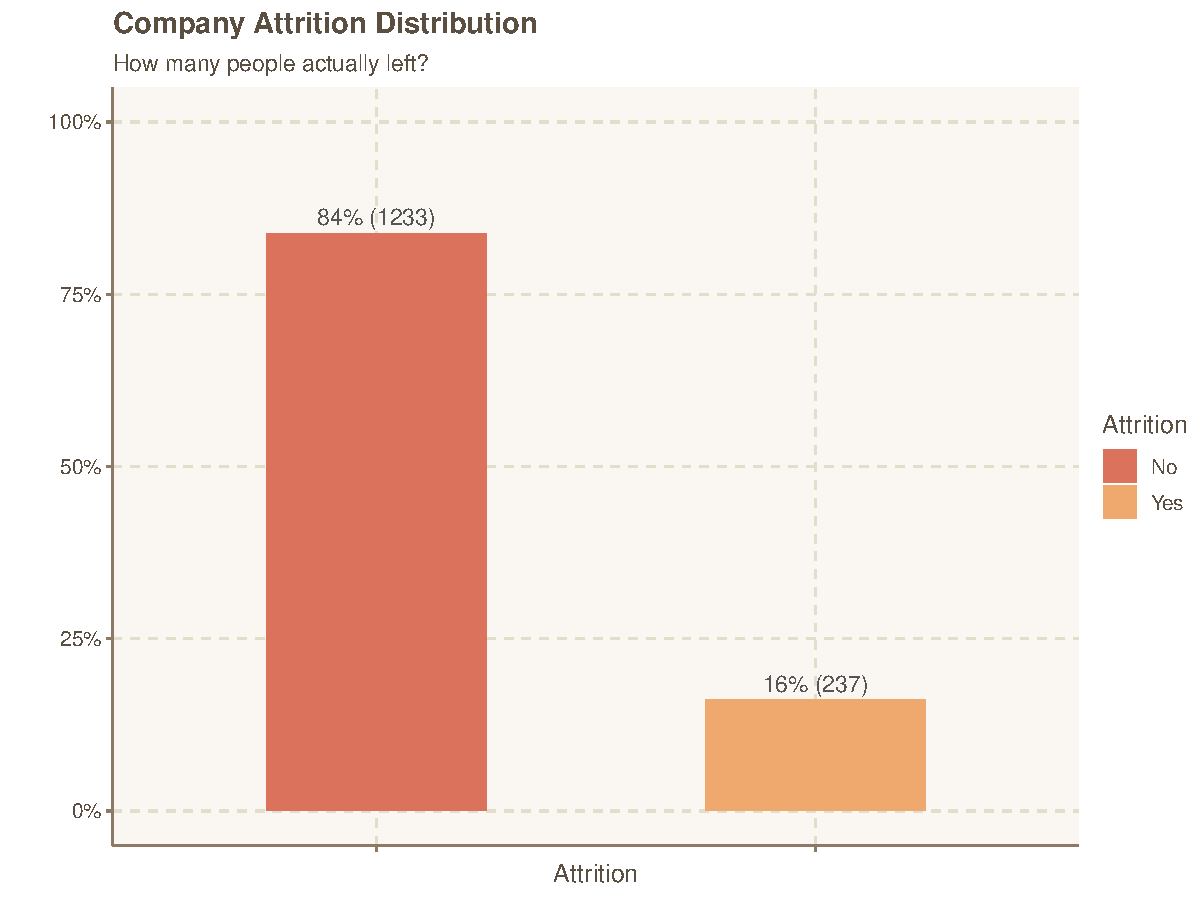
\includegraphics{figures/Overall Attrition Distribution-1.pdf}

Quick Takeaways:

\begin{itemize}
\tightlist
\item
  Organization had a 16\% attrition rate with 237 people having left.
\item
  Imbalance between those who left and those who didn't.
\end{itemize}

\textbf{Attrition Within Job Role}

\begin{Shaded}
\begin{Highlighting}[]
\NormalTok{f_data }\OperatorTok
\StringTok{  }\KeywordTok{group_by}\NormalTok{(JobRole) }\OperatorTok
\StringTok{  }\KeywordTok{count}\NormalTok{(Attrition) }\OperatorTok
\StringTok{  }\KeywordTok{mutate}\NormalTok{(}\DataTypeTok{pct =} \KeywordTok{prop.table}\NormalTok{(n)) }\OperatorTok
\StringTok{  }\KeywordTok{mutate}\NormalTok{(}\DataTypeTok{name =} \KeywordTok{paste}\NormalTok{(}\KeywordTok{round}\NormalTok{(pct,}\DecValTok{2}\NormalTok{)}\OperatorTok{*}\DecValTok{100}\NormalTok{,}\StringTok{"%"}\NormalTok{, }\DataTypeTok{sep =} \StringTok{""}\NormalTok{)) }\OperatorTok\StringTok{ }
\StringTok{  }\KeywordTok{mutate}\NormalTok{(}\DataTypeTok{JobRole =} \KeywordTok{gsub}\NormalTok{(}\StringTok{" "}\NormalTok{, }\StringTok{"}\CharTok{\textbackslash{}n}\StringTok{"}\NormalTok{, JobRole)) }\OperatorTok
\StringTok{  }\KeywordTok{subset}\NormalTok{(Attrition }\OperatorTok{==}\StringTok{ "Yes"}\NormalTok{) }\OperatorTok
\StringTok{  }\KeywordTok{ggplot}\NormalTok{(}\KeywordTok{aes}\NormalTok{(}\DataTypeTok{x =} \KeywordTok{reorder}\NormalTok{(JobRole, }\OperatorTok{-}\NormalTok{pct), }\DataTypeTok{y =}\NormalTok{ pct)) }\OperatorTok{+}\StringTok{ }
\StringTok{  }\KeywordTok{geom_point}\NormalTok{(}\DataTypeTok{size =} \DecValTok{5}\NormalTok{, }\KeywordTok{aes}\NormalTok{(}\DataTypeTok{y =}\NormalTok{ pct)) }\OperatorTok{+}\StringTok{ }
\StringTok{  }\KeywordTok{geom_segment}\NormalTok{(}\KeywordTok{aes}\NormalTok{(}\DataTypeTok{x =}\NormalTok{ JobRole, }\DataTypeTok{xend=}\NormalTok{ JobRole, }\DataTypeTok{y =} \DecValTok{0}\NormalTok{, }\DataTypeTok{yend =}\NormalTok{ pct),}
    \DataTypeTok{size =} \FloatTok{1.2}\NormalTok{, }\DataTypeTok{linetype =} \DecValTok{1}\NormalTok{, }\DataTypeTok{alpha =} \FloatTok{.8}\NormalTok{, }\DataTypeTok{color =} \StringTok{"#8d7a64"}\NormalTok{) }\OperatorTok{+}\StringTok{ }
\StringTok{  }\KeywordTok{labs}\NormalTok{(}\DataTypeTok{title =} \StringTok{"Attrition Percentage Within Each Job Role"}\NormalTok{,}
    \DataTypeTok{subtitle =} \StringTok{"What percentage of people left within each job role?"}\NormalTok{,}
    \DataTypeTok{x =} \StringTok{"Job Roles"}\NormalTok{, }
    \DataTypeTok{y =} \StringTok{"% of Attrition"}\NormalTok{) }\OperatorTok{+}\StringTok{ }
\StringTok{  }\KeywordTok{geom_text}\NormalTok{(}\KeywordTok{aes}\NormalTok{(}\DataTypeTok{label =}\NormalTok{ name, }\DataTypeTok{x =}\NormalTok{ JobRole, }\DataTypeTok{y=}\NormalTok{ pct), }\DataTypeTok{vjust =} \FloatTok{-1.8}\NormalTok{) }\OperatorTok{+}\StringTok{ }
\StringTok{  }\KeywordTok{scale_y_continuous}\NormalTok{(}\DataTypeTok{labels =}\NormalTok{ scales}\OperatorTok{::}\KeywordTok{percent_format}\NormalTok{(}\DataTypeTok{accuracy =} \DecValTok{1}\NormalTok{), }\DataTypeTok{limits =} \KeywordTok{c}\NormalTok{(}\DecValTok{0}\NormalTok{, }\FloatTok{.5}\NormalTok{))}
\end{Highlighting}
\end{Shaded}

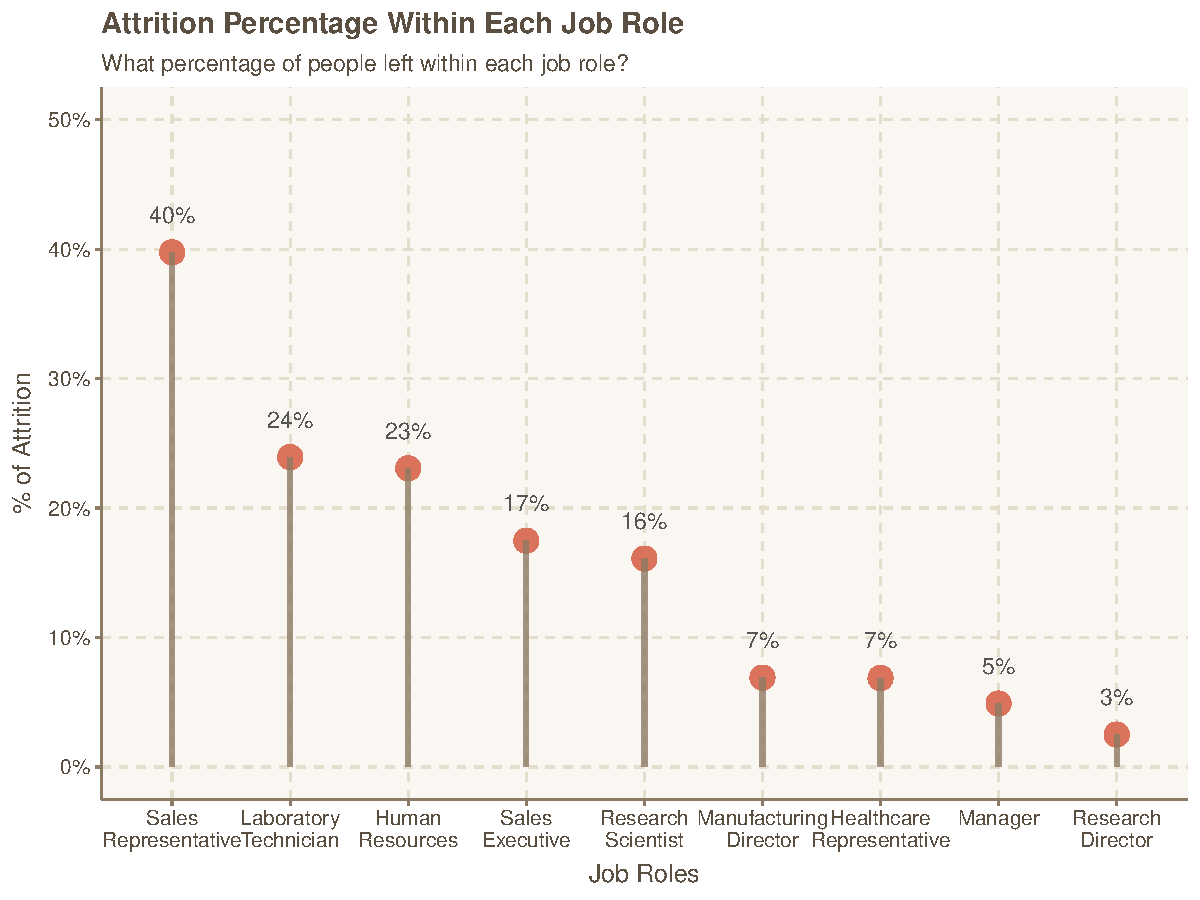
\includegraphics{figures/Attrition Within Job Role-1.pdf}

\textbf{Quick Takeaways:}

\begin{itemize}
\tightlist
\item
  Sales representatives had the highest percentage of people leaving
  while research director and managers had the lowest percentage.
\end{itemize}

\textbf{Attrition Within Each Department}

\begin{Shaded}
\begin{Highlighting}[]
\NormalTok{f_data }\OperatorTok
\StringTok{  }\KeywordTok{group_by}\NormalTok{(Department) }\OperatorTok
\StringTok{  }\KeywordTok{count}\NormalTok{(Attrition) }\OperatorTok
\StringTok{  }\KeywordTok{mutate}\NormalTok{(}\DataTypeTok{pct =} \KeywordTok{prop.table}\NormalTok{(n)) }\OperatorTok
\StringTok{  }\KeywordTok{mutate}\NormalTok{(}\DataTypeTok{name =} \KeywordTok{paste}\NormalTok{(}\KeywordTok{round}\NormalTok{(pct,}\DecValTok{2}\NormalTok{)}\OperatorTok{*}\DecValTok{100}\NormalTok{,}\StringTok{"%"}\NormalTok{, }\DataTypeTok{sep =} \StringTok{""}\NormalTok{)) }\OperatorTok\StringTok{ }
\StringTok{  }\KeywordTok{mutate}\NormalTok{(}\DataTypeTok{Department =} \KeywordTok{gsub}\NormalTok{(}\StringTok{" "}\NormalTok{, }\StringTok{"}\CharTok{\textbackslash{}n}\StringTok{"}\NormalTok{, Department)) }\OperatorTok
\StringTok{  }\KeywordTok{subset}\NormalTok{(Attrition }\OperatorTok{==}\StringTok{ "Yes"}\NormalTok{) }\OperatorTok
\StringTok{  }\KeywordTok{ggplot}\NormalTok{(}\KeywordTok{aes}\NormalTok{(}\DataTypeTok{x =} \KeywordTok{reorder}\NormalTok{(Department, }\OperatorTok{-}\NormalTok{pct), }\DataTypeTok{y =}\NormalTok{ pct)) }\OperatorTok{+}\StringTok{ }
\StringTok{  }\KeywordTok{geom_point}\NormalTok{(}\DataTypeTok{size =} \DecValTok{5}\NormalTok{, }\KeywordTok{aes}\NormalTok{(}\DataTypeTok{y =}\NormalTok{ pct)) }\OperatorTok{+}\StringTok{ }
\StringTok{  }\KeywordTok{geom_segment}\NormalTok{(}\KeywordTok{aes}\NormalTok{(}\DataTypeTok{x =}\NormalTok{ Department, }\DataTypeTok{xend=}\NormalTok{ Department, }\DataTypeTok{y =} \DecValTok{0}\NormalTok{, }\DataTypeTok{yend =}\NormalTok{ pct),}
    \DataTypeTok{size =} \FloatTok{1.2}\NormalTok{, }\DataTypeTok{linetype =} \DecValTok{1}\NormalTok{, }\DataTypeTok{alpha =} \FloatTok{.8}\NormalTok{, }\DataTypeTok{color =} \StringTok{"#8d7a64"}\NormalTok{) }\OperatorTok{+}\StringTok{ }
\StringTok{  }\KeywordTok{labs}\NormalTok{(}\DataTypeTok{title =} \StringTok{"Attrition Within Each Department"}\NormalTok{,}
    \DataTypeTok{subtitle =} \StringTok{"What percentage of people left within each department?"}\NormalTok{,}
    \DataTypeTok{x =} \StringTok{"Departments"}\NormalTok{, }
    \DataTypeTok{y =} \StringTok{"% of Attrition"}\NormalTok{) }\OperatorTok{+}\StringTok{ }
\StringTok{  }\KeywordTok{geom_text}\NormalTok{(}\KeywordTok{aes}\NormalTok{(}\DataTypeTok{label =}\NormalTok{ name, }\DataTypeTok{x =}\NormalTok{ Department, }\DataTypeTok{y=}\NormalTok{ pct), }\DataTypeTok{vjust =} \FloatTok{-1.8}\NormalTok{) }\OperatorTok{+}\StringTok{ }
\StringTok{  }\KeywordTok{scale_y_continuous}\NormalTok{(}\DataTypeTok{labels =}\NormalTok{ scales}\OperatorTok{::}\KeywordTok{percent_format}\NormalTok{(}\DataTypeTok{accuracy =} \DecValTok{1}\NormalTok{), }\DataTypeTok{limits =} \KeywordTok{c}\NormalTok{(}\DecValTok{0}\NormalTok{, }\FloatTok{.5}\NormalTok{))}
\end{Highlighting}
\end{Shaded}

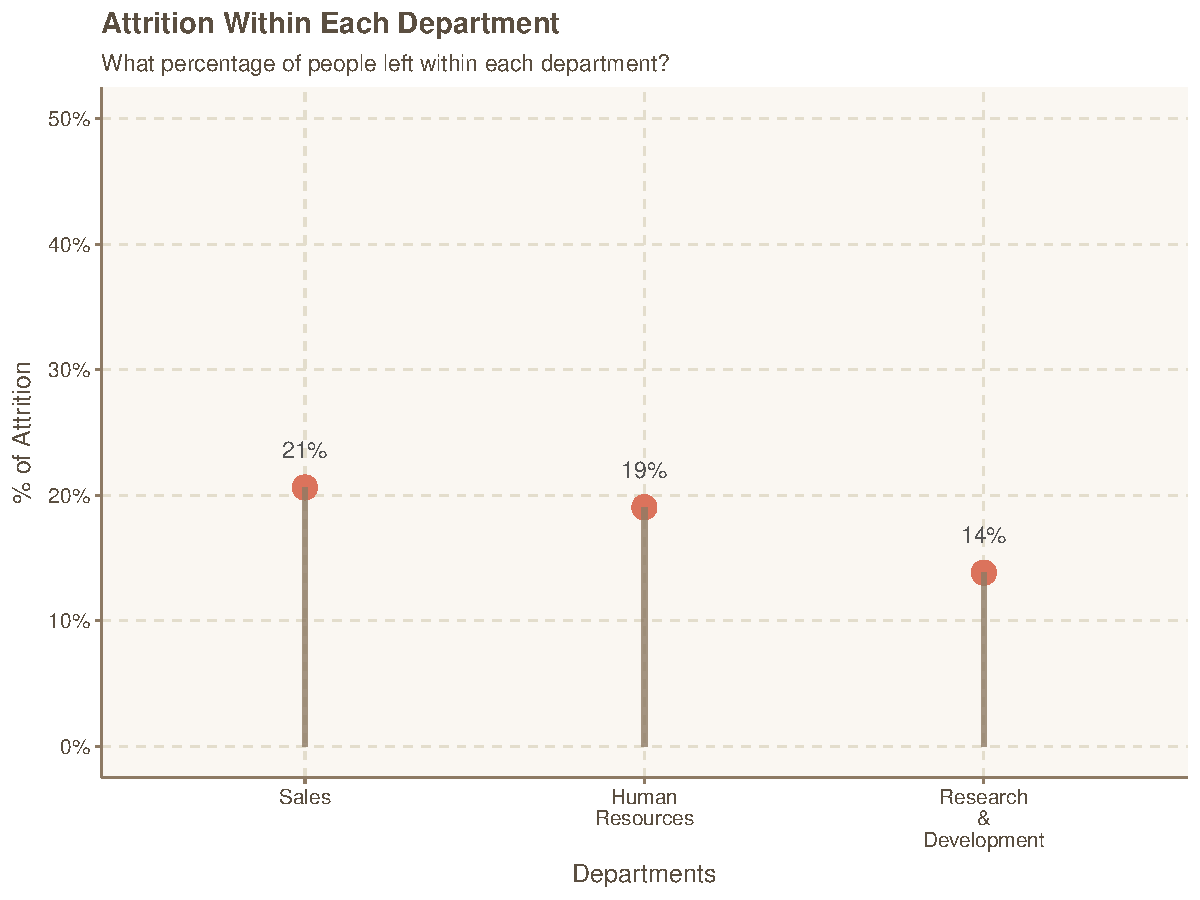
\includegraphics{figures/Attrition Within Each Department-1.pdf}

\textbf{Quick Takeaways:}

\begin{itemize}
\tightlist
\item
  Unlike job roles, each department didn't differ as much in terms of
  the percentage of people leaving. This leads me to think that other
  factors rather than departmental issues are more likely to affect
  attrition
\end{itemize}

\textbf{Attrition Within Job Level}

\begin{Shaded}
\begin{Highlighting}[]
\NormalTok{f_data }\OperatorTok
\StringTok{  }\KeywordTok{group_by}\NormalTok{(JobLevel) }\OperatorTok
\StringTok{  }\KeywordTok{count}\NormalTok{(Attrition) }\OperatorTok
\StringTok{  }\KeywordTok{mutate}\NormalTok{(}\DataTypeTok{pct =} \KeywordTok{prop.table}\NormalTok{(n)) }\OperatorTok
\StringTok{  }\KeywordTok{mutate}\NormalTok{(}\DataTypeTok{name =} \KeywordTok{paste}\NormalTok{(}\KeywordTok{round}\NormalTok{(pct,}\DecValTok{2}\NormalTok{)}\OperatorTok{*}\DecValTok{100}\NormalTok{,}\StringTok{"%"}\NormalTok{, }\DataTypeTok{sep =} \StringTok{""}\NormalTok{)) }\OperatorTok\StringTok{ }
\StringTok{  }\KeywordTok{mutate}\NormalTok{(}\DataTypeTok{JobLevel =} \KeywordTok{paste}\NormalTok{(}\StringTok{"Level"}\NormalTok{, JobLevel)) }\OperatorTok
\StringTok{  }\KeywordTok{subset}\NormalTok{(Attrition }\OperatorTok{==}\StringTok{ "Yes"}\NormalTok{) }\OperatorTok
\StringTok{  }\KeywordTok{ggplot}\NormalTok{(}\KeywordTok{aes}\NormalTok{(}\DataTypeTok{x =}\NormalTok{ JobLevel, }\DataTypeTok{y =}\NormalTok{ pct)) }\OperatorTok{+}\StringTok{ }
\StringTok{  }\KeywordTok{geom_point}\NormalTok{(}\DataTypeTok{size =} \DecValTok{6}\NormalTok{, }\KeywordTok{aes}\NormalTok{(}\DataTypeTok{y =}\NormalTok{ pct)) }\OperatorTok{+}\StringTok{ }
\StringTok{  }\KeywordTok{geom_segment}\NormalTok{(}\KeywordTok{aes}\NormalTok{(}\DataTypeTok{x =}\NormalTok{ JobLevel, }\DataTypeTok{xend=}\NormalTok{ JobLevel, }\DataTypeTok{y =} \DecValTok{0}\NormalTok{, }\DataTypeTok{yend =}\NormalTok{ pct),}
    \DataTypeTok{size =} \FloatTok{1.2}\NormalTok{, }\DataTypeTok{linetype =} \DecValTok{1}\NormalTok{, }\DataTypeTok{alpha =} \FloatTok{.8}\NormalTok{, }\DataTypeTok{color =} \StringTok{"#8d7a64"}\NormalTok{) }\OperatorTok{+}\StringTok{ }
\StringTok{  }\KeywordTok{labs}\NormalTok{(}\DataTypeTok{title =} \StringTok{"Attrition Percentage Within Job Level"}\NormalTok{,}
    \DataTypeTok{subtitle =} \StringTok{"What percentage of people left within each job level?"}\NormalTok{,}
    \DataTypeTok{x =} \StringTok{"Job Levels"}\NormalTok{, }
    \DataTypeTok{y =} \StringTok{"% of Attrition"}\NormalTok{) }\OperatorTok{+}\StringTok{ }
\StringTok{  }\KeywordTok{geom_text}\NormalTok{(}\KeywordTok{aes}\NormalTok{(}\DataTypeTok{label =}\NormalTok{ name, }\DataTypeTok{x =}\NormalTok{ JobLevel, }\DataTypeTok{y=}\NormalTok{ pct), }\DataTypeTok{vjust =} \FloatTok{-1.8}\NormalTok{) }\OperatorTok{+}\StringTok{ }
\StringTok{  }\KeywordTok{scale_y_continuous}\NormalTok{(}\DataTypeTok{labels =}\NormalTok{ scales}\OperatorTok{::}\KeywordTok{percent_format}\NormalTok{(}\DataTypeTok{accuracy =} \DecValTok{1}\NormalTok{), }\DataTypeTok{limits =} \KeywordTok{c}\NormalTok{(}\DecValTok{0}\NormalTok{, }\FloatTok{.5}\NormalTok{)) }
\end{Highlighting}
\end{Shaded}

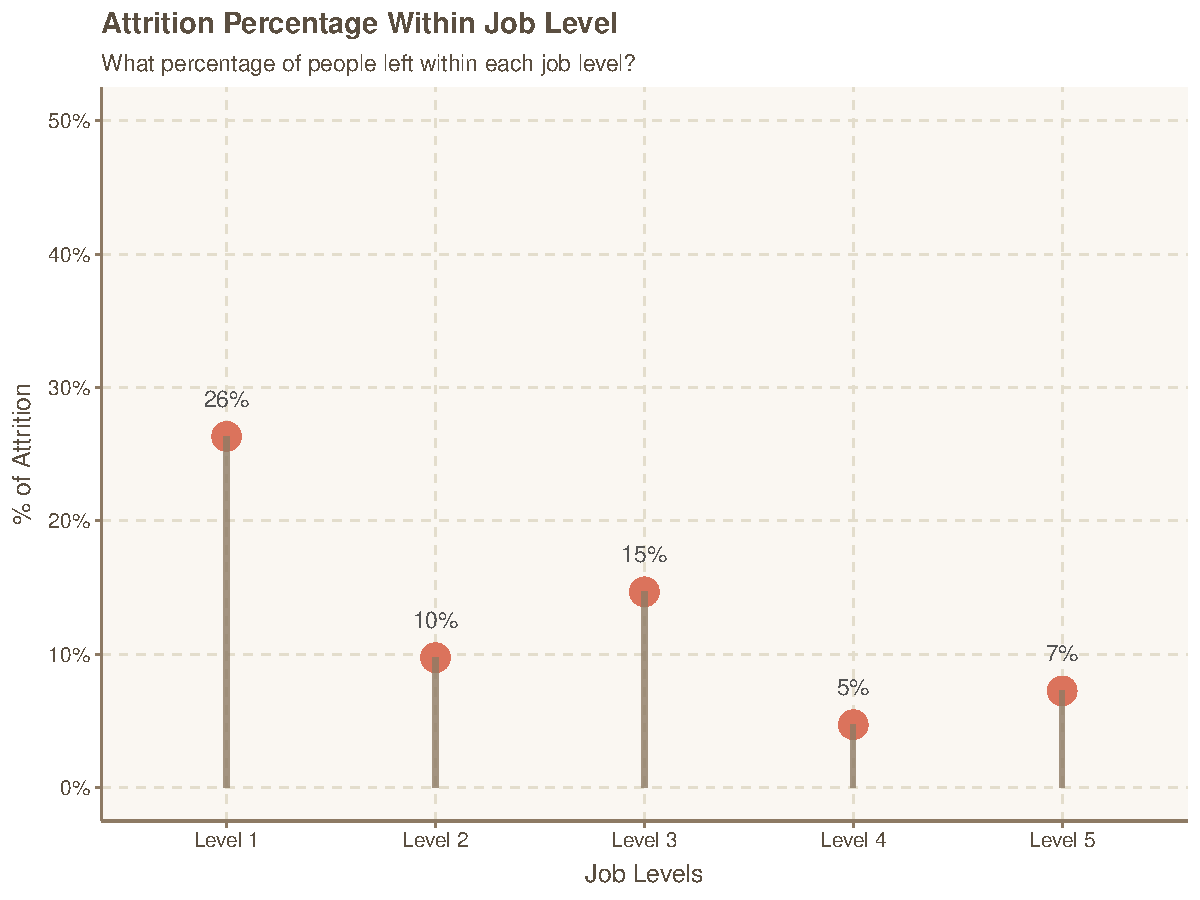
\includegraphics{figures/Attrition Within Job Level-1.pdf}

\textbf{Quick Takeaways:}

\begin{itemize}
\tightlist
\item
  As expected people from the lowest level are leaving than those in
  higher levels. However, it may be worth while to investigate why there
  was a slight jump in attrition from level 2 to level 3.
\end{itemize}

~ ~

\hypertarget{demographics-analysis}{%
\subsection{Demographics Analysis}\label{demographics-analysis}}

Therefore, I will evaluate if people in different \textbf{age} and
\textbf{gender} are leaving at different rates. I will ask the
following:

\begin{itemize}
\tightlist
\item
  Are people in certain gender or age groups leaving at higher rates?
\item
  Are people in certain gender or age groups in a particular job role or
  job level leaving at higher rates?
\end{itemize}

~ ~

\hypertarget{demographics-analysis-1-age}{%
\paragraph{Demographics Analysis 1:
Age}\label{demographics-analysis-1-age}}

\textbf{Summary:} After looking at the attrition distribution separated
by age groups and then age groups within job roles, departments, and job
levels here are my following insights:

\begin{enumerate}
\def\labelenumi{\arabic{enumi}.}
\item
  The average employee age is 39.
\item
  \textbf{Approximately 55\% of all of the attrition occurred between
  individuals ages 18-32} This seems to indicate that the company is
  struggling to maintain younger talent than older talent.
\item
  The company lost \textbf{36\% of employees within the 18-25 bracket}
  while losing \textbf{22\% of all employees within the 26-32 bracket.}
\item
  The loss of young talent was \textbf{specially bad for those who are
  the sales representatives role and in for those in level 1.}
\end{enumerate}

\textbf{Final thoughts:} The most concerning irregularities comes when
looking at the \textbf{loss of young talent.} It may be possible that
there is a culture or policy unfavorable to younger individuals. Further
analysis on why younger talents are leaving will be evaluated when
looking at income and satisfaction ratings. This high attrition rate may
be fine if those who are leaving are lower performers. However, it is a
serious issue if high performers are leaving as well. Unfortunately due
to the way the performance ratings were done, it would be nearly
impossible to tell (everyone scored either a 3 or 4 on performance
rating which means not enough variability exists).

~

\hypertarget{supporting-analysis-for-demgraphic-analysis-1-age}{%
\subsubsection{Supporting Analysis for Demgraphic Analysis 1:
Age}\label{supporting-analysis-for-demgraphic-analysis-1-age}}

~

\textbf{Age Distribution}

\begin{Shaded}
\begin{Highlighting}[]
\KeywordTok{ggthemr}\NormalTok{(}\StringTok{"dust"}\NormalTok{)}
\NormalTok{f_data }\OperatorTok
\StringTok{  }\KeywordTok{ggplot}\NormalTok{(}\KeywordTok{aes}\NormalTok{(}\DataTypeTok{x =}\NormalTok{ Age, }\DataTypeTok{fill =}\NormalTok{ Attrition)) }\OperatorTok{+}\StringTok{ }
\StringTok{  }\KeywordTok{geom_histogram}\NormalTok{(}\DataTypeTok{binwidth =} \DecValTok{2}\NormalTok{) }\OperatorTok{+}\StringTok{ }
\StringTok{  }\KeywordTok{geom_segment}\NormalTok{(}\KeywordTok{aes}\NormalTok{(}\DataTypeTok{x =} \KeywordTok{mean}\NormalTok{(Age), }\DataTypeTok{y =} \DecValTok{0}\NormalTok{, }\DataTypeTok{xend =} \KeywordTok{mean}\NormalTok{(Age), }\DataTypeTok{yend =} \OtherTok{Inf}\NormalTok{, }\DataTypeTok{linetype =} \StringTok{"Mean"}\NormalTok{), }\DataTypeTok{col =} \StringTok{"#484848"}\NormalTok{, }\DataTypeTok{lwd =} \FloatTok{1.2}\NormalTok{) }\OperatorTok{+}
\StringTok{  }\KeywordTok{labs}\NormalTok{(}\DataTypeTok{x =} \StringTok{"Individual's Age"}\NormalTok{, }\DataTypeTok{y =} \StringTok{"count"}\NormalTok{, }\DataTypeTok{title =} \StringTok{"Age Distribution"}\NormalTok{, }\DataTypeTok{subtitle =} \StringTok{"What is the age distribution of the organization?"}\NormalTok{) }\OperatorTok{+}\StringTok{ }
\StringTok{  }\KeywordTok{scale_linetype_manual}\NormalTok{(}\DataTypeTok{name =} \StringTok{"Line"}\NormalTok{, }\DataTypeTok{values =} \KeywordTok{c}\NormalTok{(}\StringTok{"Mean"}\NormalTok{ =}\StringTok{ }\DecValTok{3}\NormalTok{)) }\OperatorTok{+}
\StringTok{  }\KeywordTok{guides}\NormalTok{(}\DataTypeTok{fill =} \KeywordTok{guide_legend}\NormalTok{(}\DataTypeTok{order =} \DecValTok{1}\NormalTok{), }\DataTypeTok{linetype =} \KeywordTok{guide_legend}\NormalTok{(}\DataTypeTok{order =} \DecValTok{2}\NormalTok{))}
\end{Highlighting}
\end{Shaded}

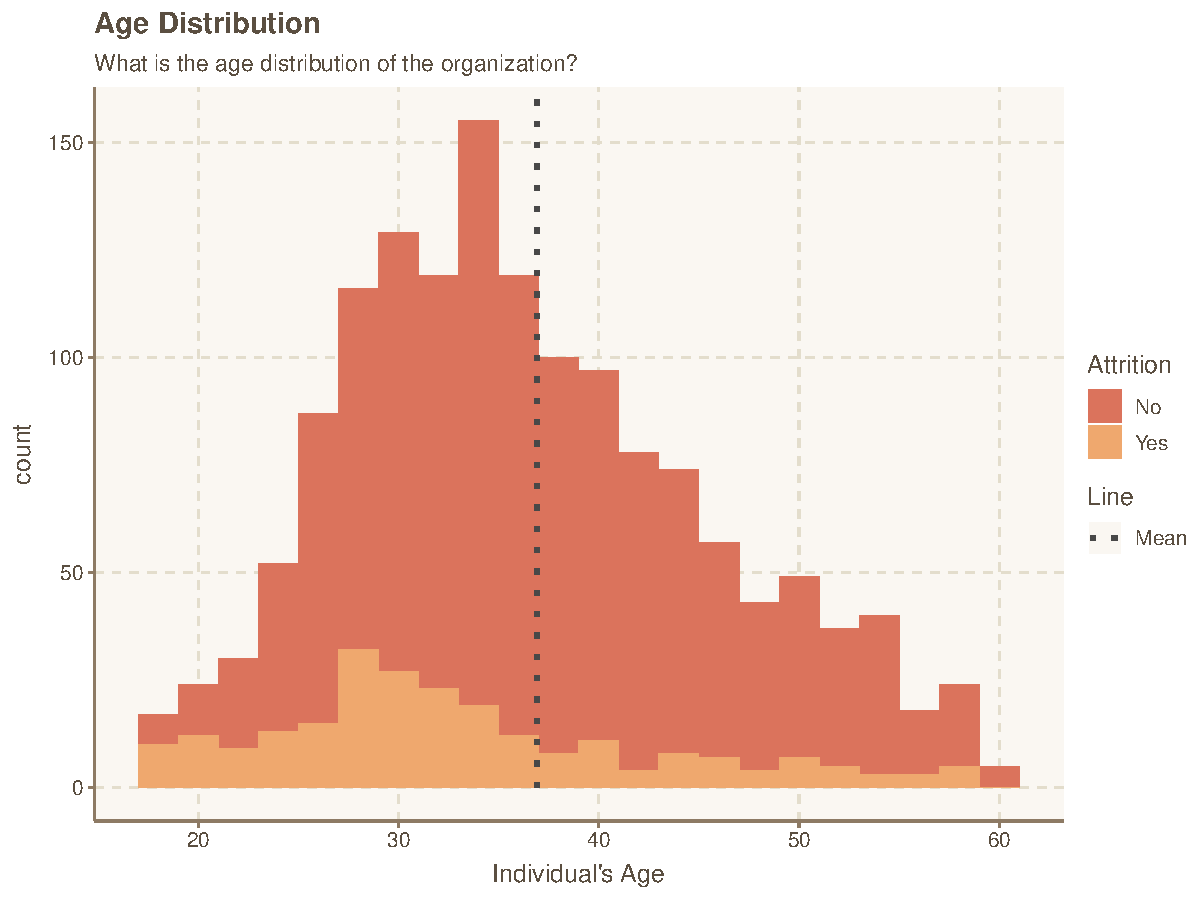
\includegraphics{figures/Age Distribution-1.pdf}

Quick Takeaways:

\begin{itemize}
\tightlist
\item
  The average age of the employees is approximately 39.
\item
  Overall, the organization has a large number of employees that are in
  their late twenties to mid 40s.
\item
  Although not definitive, there does seem to be a higher percentage of
  those in their 20s leaving the organization.
\end{itemize}

\textbf{Creating Age Brackets}

\begin{Shaded}
\begin{Highlighting}[]
\NormalTok{AgeQ <-}\StringTok{ }\KeywordTok{split_quantile}\NormalTok{(f_data}\OperatorTok{$}\NormalTok{Age, }\DataTypeTok{type =} \DecValTok{4}\NormalTok{)}
\NormalTok{AgeQ <-}\StringTok{ }\KeywordTok{as.factor}\NormalTok{(}\KeywordTok{cut}\NormalTok{(f_data}\OperatorTok{$}\NormalTok{Age, }\DataTypeTok{breaks =} \DecValTok{6}\NormalTok{, }
  \DataTypeTok{labels =} \KeywordTok{c}\NormalTok{(}\StringTok{"18-25"}\NormalTok{, }\StringTok{"26-32"}\NormalTok{, }\StringTok{"33-39"}\NormalTok{, }\StringTok{"40-46"}\NormalTok{, }\StringTok{"47-53"}\NormalTok{, }\StringTok{"54-60"}\NormalTok{)))}
\KeywordTok{table}\NormalTok{(AgeQ)}
\end{Highlighting}
\end{Shaded}

\begin{verbatim}
## AgeQ
## 18-25 26-32 33-39 40-46 47-53 54-60 
##   123   393   432   282   153    87
\end{verbatim}

\textbf{Attrition by Age Brackets}

\begin{Shaded}
\begin{Highlighting}[]
\NormalTok{f_data }\OperatorTok
\StringTok{  }\KeywordTok{select}\NormalTok{(Age, Attrition) }\OperatorTok
\StringTok{  }\KeywordTok{mutate}\NormalTok{(}\DataTypeTok{AgeQ =}\NormalTok{ AgeQ) }\OperatorTok
\StringTok{  }\KeywordTok{filter}\NormalTok{(Attrition }\OperatorTok{==}\StringTok{ "Yes"}\NormalTok{) }\OperatorTok
\StringTok{  }\KeywordTok{group_by}\NormalTok{(AgeQ) }\OperatorTok
\StringTok{  }\KeywordTok{summarise}\NormalTok{(}\DataTypeTok{count =} \KeywordTok{n}\NormalTok{()) }\OperatorTok
\StringTok{  }\KeywordTok{mutate}\NormalTok{(}\DataTypeTok{pct =} \KeywordTok{prop.table}\NormalTok{(count),}
    \DataTypeTok{label=} \KeywordTok{paste0}\NormalTok{(}\KeywordTok{round}\NormalTok{(pct}\OperatorTok{*}\DecValTok{100}\NormalTok{,}\DecValTok{0}\NormalTok{), }\StringTok{"%"}\NormalTok{,}\StringTok{" ("}\NormalTok{, count, }\StringTok{")"}\NormalTok{, }\DataTypeTok{sep =} \StringTok{""}\NormalTok{)) }\OperatorTok
\StringTok{  }\KeywordTok{ggplot}\NormalTok{(}\KeywordTok{aes}\NormalTok{(}\DataTypeTok{x =}\NormalTok{ AgeQ, }\DataTypeTok{y =}\NormalTok{ pct)) }\OperatorTok{+}
\StringTok{  }\KeywordTok{geom_bar}\NormalTok{(}\DataTypeTok{stat =} \StringTok{"identity"}\NormalTok{) }\OperatorTok{+}\StringTok{ }
\StringTok{  }\KeywordTok{geom_text}\NormalTok{(}\KeywordTok{aes}\NormalTok{(}\DataTypeTok{x =}\NormalTok{ AgeQ, }\DataTypeTok{y =}\NormalTok{ pct, }\DataTypeTok{label =}\NormalTok{ label),}
    \DataTypeTok{vjust =} \DecValTok{-1}\NormalTok{) }\OperatorTok{+}\StringTok{ }
\StringTok{  }\KeywordTok{scale_y_continuous}\NormalTok{(}\DataTypeTok{labels =}\NormalTok{ scales}\OperatorTok{::}\KeywordTok{percent_format}\NormalTok{(}\DataTypeTok{accuracy =} \DecValTok{1}\NormalTok{), }\DataTypeTok{limits =} \KeywordTok{c}\NormalTok{(}\DecValTok{0}\NormalTok{,.}\DecValTok{5}\NormalTok{)) }\OperatorTok{+}
\StringTok{  }\KeywordTok{labs}\NormalTok{(}\DataTypeTok{title =} \StringTok{"Company Attrition Distribution By Age Brackets"}\NormalTok{,}
    \DataTypeTok{subtitle =} \StringTok{"How many people left within each age bracket?"}\NormalTok{, }
    \DataTypeTok{x =} \StringTok{"Age Brackets"}\NormalTok{,}
    \DataTypeTok{y =} \StringTok{""}\NormalTok{)}
\end{Highlighting}
\end{Shaded}

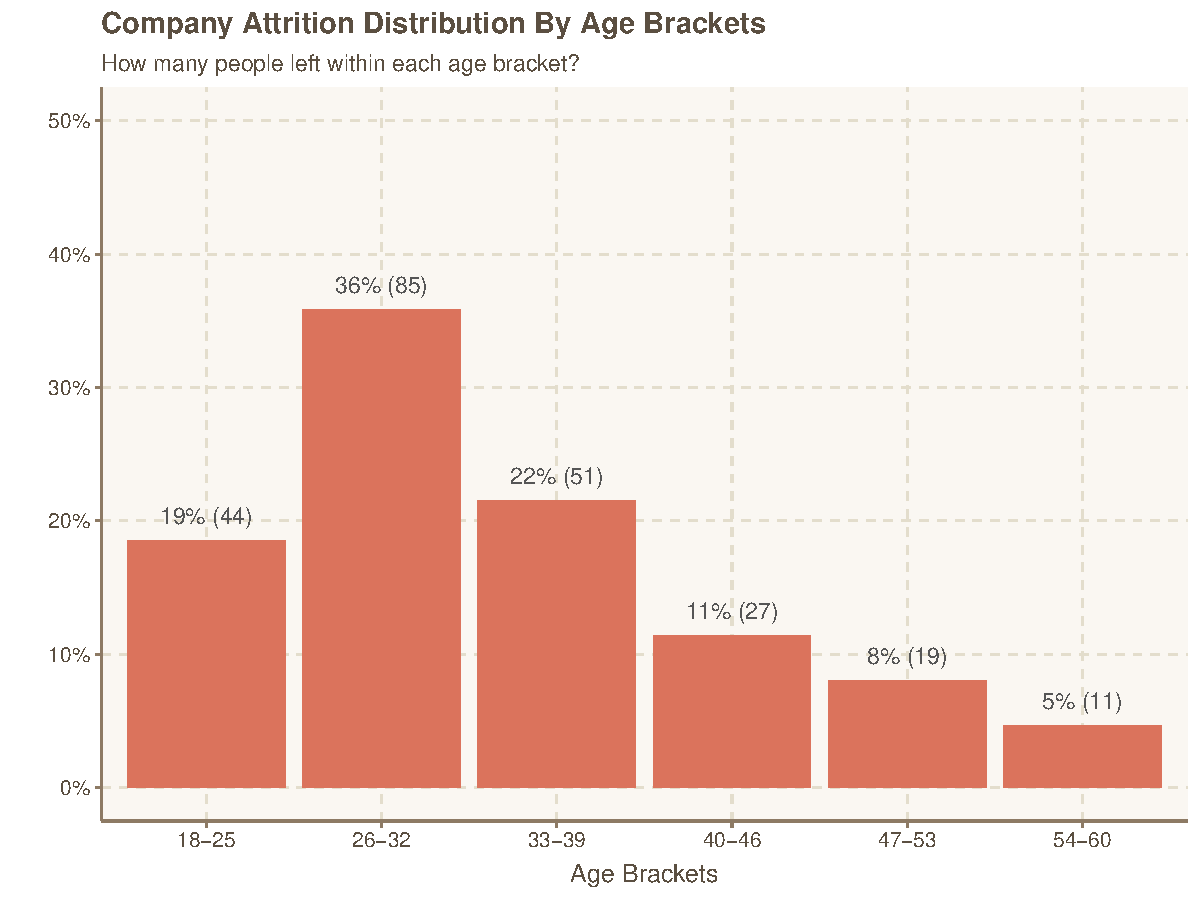
\includegraphics{figures/Attrition Distribtuion by Age Brackets-1.pdf}

Quick Takeaways:

\begin{itemize}
\tightlist
\item
  Approximate 55\% of all attrition comes from younger employees between
  18-32. Overall, it seems as though the company is struggling to
  maintain younger talent verses older talent.
\item
  The organization seems to be doing well in keeping employees between
  the age 33-39 considering only a 22\% of attrition for the
  organization's largest group. The 33-39 age bracket contains their
  largest number of employees with 432 employees approximately 29.4\% of
  the entire workforce.
\end{itemize}

\textbf{Attrition Within Each Age Brackets}

\begin{Shaded}
\begin{Highlighting}[]
\NormalTok{f_data }\OperatorTok
\StringTok{  }\KeywordTok{select}\NormalTok{(Age, Attrition) }\OperatorTok
\StringTok{  }\KeywordTok{mutate}\NormalTok{(}\DataTypeTok{AgeQ =}\NormalTok{ AgeQ) }\OperatorTok
\StringTok{  }\KeywordTok{group_by}\NormalTok{(AgeQ, Attrition) }\OperatorTok
\StringTok{  }\KeywordTok{summarise}\NormalTok{(}\DataTypeTok{count =} \KeywordTok{n}\NormalTok{()) }\OperatorTok
\StringTok{  }\KeywordTok{group_by}\NormalTok{(AgeQ) }\OperatorTok
\StringTok{  }\KeywordTok{mutate}\NormalTok{(}\DataTypeTok{pct =} \KeywordTok{prop.table}\NormalTok{(count),}
    \DataTypeTok{label=} \KeywordTok{paste0}\NormalTok{(}\KeywordTok{round}\NormalTok{(pct}\OperatorTok{*}\DecValTok{100}\NormalTok{,}\DecValTok{0}\NormalTok{), }\StringTok{"%"}\NormalTok{, }\DataTypeTok{sep =} \StringTok{""}\NormalTok{)) }\OperatorTok
\StringTok{  }\KeywordTok{filter}\NormalTok{(Attrition }\OperatorTok{==}\StringTok{ "Yes"}\NormalTok{) }\OperatorTok
\StringTok{  }\KeywordTok{ggplot}\NormalTok{(}\KeywordTok{aes}\NormalTok{(}\DataTypeTok{x =}\NormalTok{ AgeQ, }\DataTypeTok{y =}\NormalTok{ pct)) }\OperatorTok{+}
\StringTok{  }\KeywordTok{geom_bar}\NormalTok{(}\DataTypeTok{stat =} \StringTok{"identity"}\NormalTok{) }\OperatorTok{+}\StringTok{ }
\StringTok{  }\KeywordTok{geom_text}\NormalTok{(}\KeywordTok{aes}\NormalTok{(}\DataTypeTok{x =}\NormalTok{ AgeQ, }\DataTypeTok{y =}\NormalTok{ pct, }\DataTypeTok{label =}\NormalTok{ label),}
    \DataTypeTok{vjust =} \DecValTok{-1}\NormalTok{) }\OperatorTok{+}\StringTok{ }
\StringTok{  }\KeywordTok{scale_y_continuous}\NormalTok{(}\DataTypeTok{labels =}\NormalTok{ scales}\OperatorTok{::}\KeywordTok{percent_format}\NormalTok{(}\DataTypeTok{accuracy =} \DecValTok{1}\NormalTok{), }
    \DataTypeTok{limits =} \KeywordTok{c}\NormalTok{(}\DecValTok{0}\NormalTok{,.}\DecValTok{5}\NormalTok{)) }\OperatorTok{+}
\StringTok{  }\KeywordTok{labs}\NormalTok{(}\DataTypeTok{title =} \StringTok{"Company Attrition Distribution Within Age Brackets"}\NormalTok{,}
    \DataTypeTok{subtitle =} \StringTok{"How many people left within each age bracket?"}\NormalTok{, }
    \DataTypeTok{x =} \StringTok{"Age Bracket"}\NormalTok{,}
    \DataTypeTok{y =} \StringTok{""}\NormalTok{)}
\end{Highlighting}
\end{Shaded}

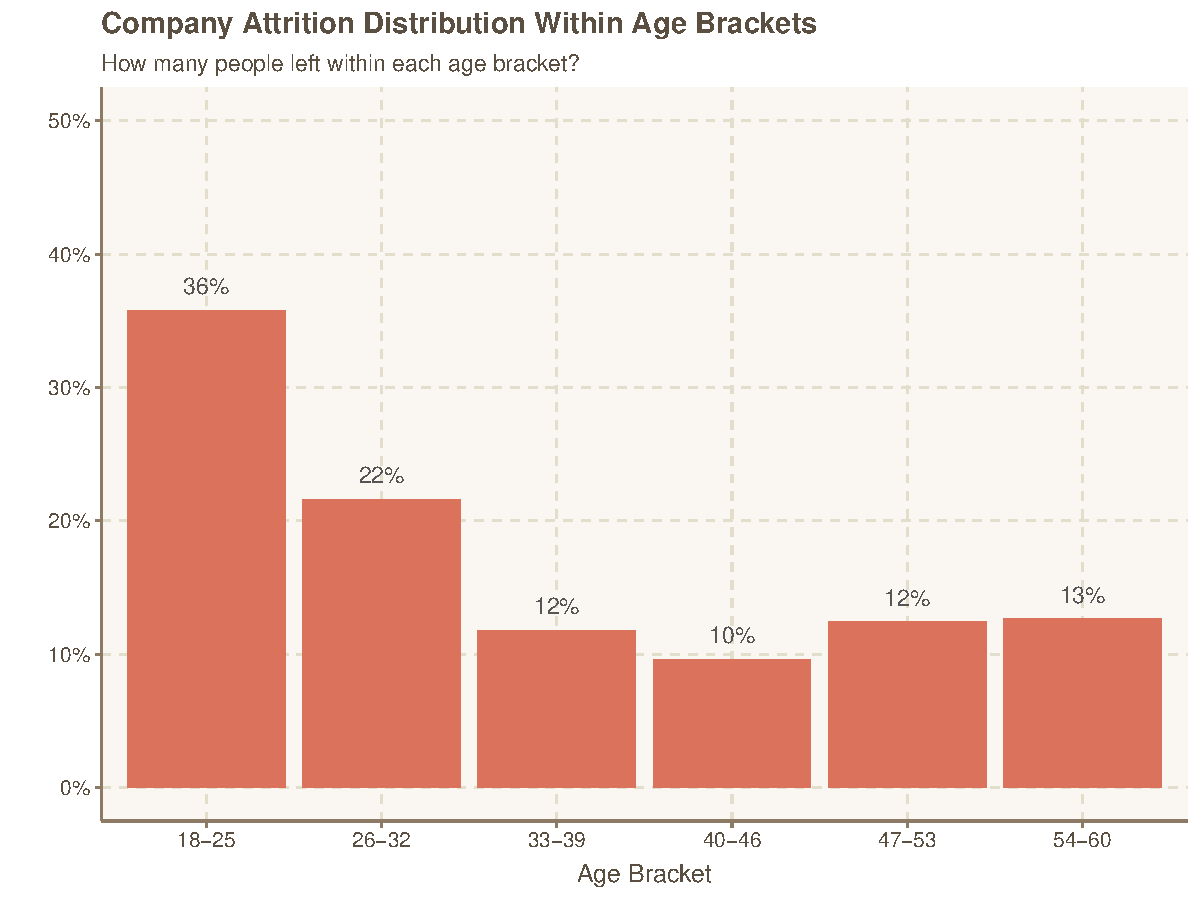
\includegraphics{figures/Attrition Within Age Brackets-1.pdf}

Quick Takeaways:

\begin{itemize}
\tightlist
\item
  Overall, 36\% of all employees in the 18-25 age bracket left in the
  given year. That percentage drops to 22\% when we go down to the next
  age bracket.
\item
  Looking at the attrition rates by age bracket and within age bracket,
  the story continues to indicate that younger people are leaving at a
  higher rate.
\end{itemize}

\textbf{Attrition Within Each Age Brackets}

\begin{Shaded}
\begin{Highlighting}[]
\NormalTok{f_data }\OperatorTok
\StringTok{  }\KeywordTok{select}\NormalTok{(Age, JobRole, Department, JobLevel, Attrition) }\OperatorTok
\StringTok{  }\KeywordTok{mutate}\NormalTok{(}\DataTypeTok{AgeQ =}\NormalTok{ AgeQ) }\OperatorTok
\StringTok{  }\KeywordTok{ggplot}\NormalTok{(}\KeywordTok{aes}\NormalTok{(}\DataTypeTok{x =}\NormalTok{ AgeQ, }\DataTypeTok{fill =}\NormalTok{ Attrition)) }\OperatorTok{+}\StringTok{ }
\StringTok{  }\KeywordTok{geom_bar}\NormalTok{() }\OperatorTok{+}
\StringTok{  }\KeywordTok{facet_wrap}\NormalTok{(}\KeywordTok{vars}\NormalTok{(JobRole)) }\OperatorTok{+}\StringTok{ }
\StringTok{  }\KeywordTok{labs}\NormalTok{(}\DataTypeTok{title =} \StringTok{"Attrition by Age and Job Role"}\NormalTok{, }
    \DataTypeTok{subtitle =} \StringTok{"Are there attribution differences between age groups in certain job roles??"}\NormalTok{, }
    \DataTypeTok{x =} \StringTok{"Age Brackets"}\NormalTok{)}
\end{Highlighting}
\end{Shaded}

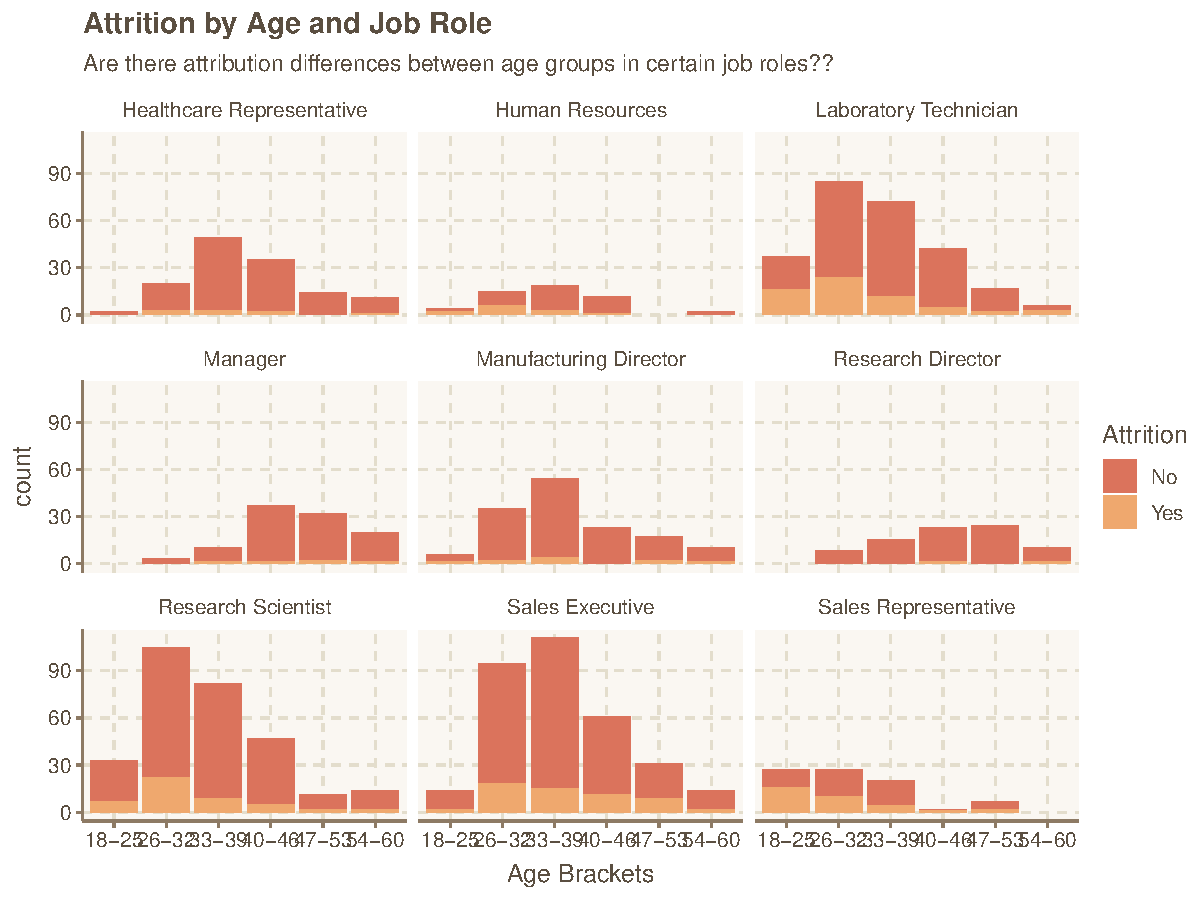
\includegraphics{figures/Age and Job Role-1.pdf}

Quick Takeaways:

\begin{itemize}
\tightlist
\item
  When we look at attrition by age and job role, things seem relatively
  normal. People are leaving proportionally to the number of people
  within the age bracket and job role.
\item
  More than 50\% of sales rep between the ages of 18-25 are leaving.
\end{itemize}

\textbf{Attrition Within Each Age Brackets and Job Level}

\begin{Shaded}
\begin{Highlighting}[]
\NormalTok{f_data }\OperatorTok
\StringTok{  }\KeywordTok{select}\NormalTok{(Age, JobLevel, Attrition) }\OperatorTok
\StringTok{  }\KeywordTok{mutate}\NormalTok{(}\DataTypeTok{AgeQ =}\NormalTok{ AgeQ) }\OperatorTok
\StringTok{  }\KeywordTok{ggplot}\NormalTok{(}\KeywordTok{aes}\NormalTok{(}\DataTypeTok{x =}\NormalTok{ AgeQ, }\DataTypeTok{fill =}\NormalTok{ Attrition)) }\OperatorTok{+}\StringTok{ }
\StringTok{  }\KeywordTok{geom_bar}\NormalTok{() }\OperatorTok{+}
\StringTok{  }\KeywordTok{facet_wrap}\NormalTok{(}\KeywordTok{vars}\NormalTok{(JobLevel)) }\OperatorTok{+}\StringTok{ }
\StringTok{  }\KeywordTok{labs}\NormalTok{(}\DataTypeTok{title =} \StringTok{"Attrition by Age and Job Level"}\NormalTok{, }
    \DataTypeTok{subtitle =} \StringTok{"Are there attribution differences between age groups in certain job levels??"}\NormalTok{)}
\end{Highlighting}
\end{Shaded}

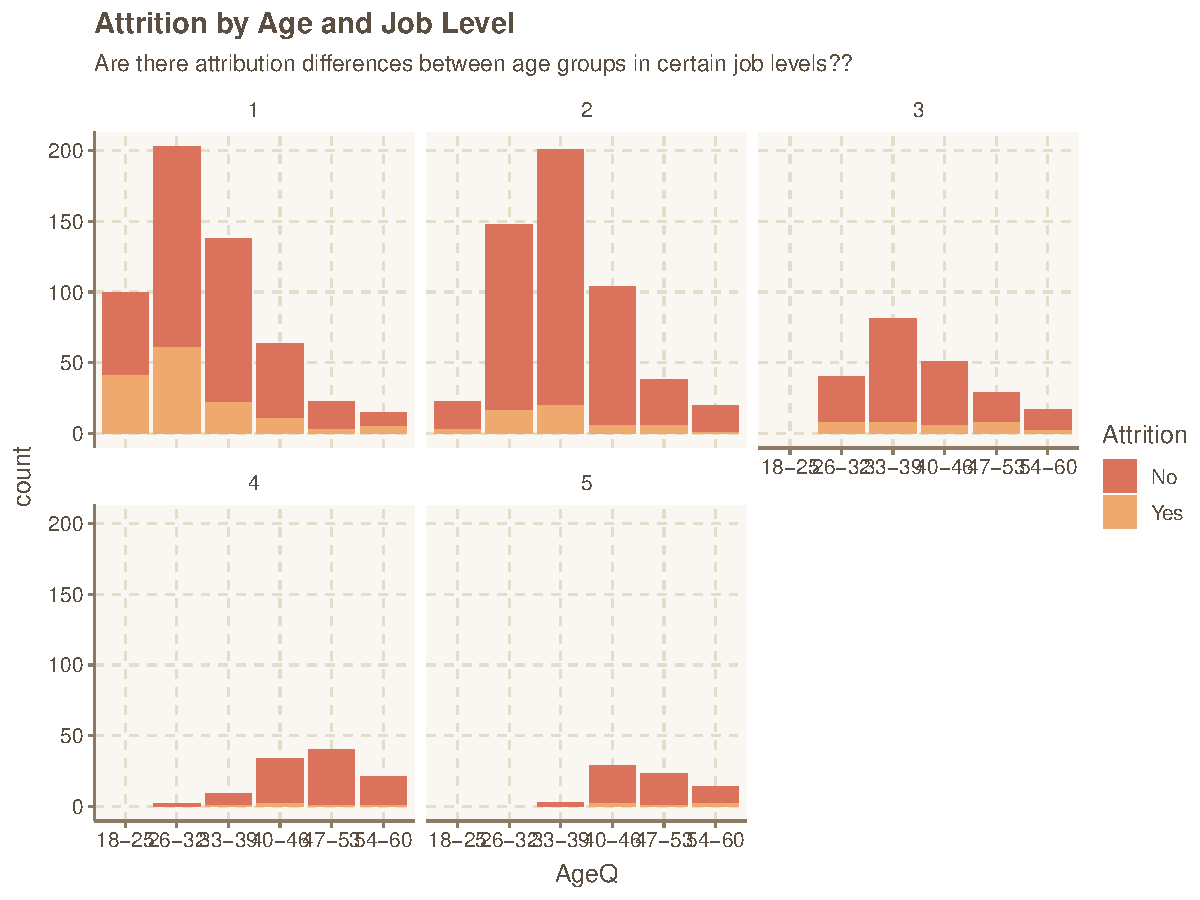
\includegraphics{figures/Age and Job Level-1.pdf}

Quick Takeaways:

\begin{itemize}
\tightlist
\item
  Individuals in the 18-25 age bracket + level 1 are leaving at a higher
  rate than those in the 26-32 age bracket + level 1.
\end{itemize}

~ ~

\hypertarget{demographics-analysis-2-gender}{%
\subsection{Demographics Analysis \#2:
Gender}\label{demographics-analysis-2-gender}}

\textbf{Summary:} After looking at the attrition distribution separated
by \textbf{gender} and then gender within job roles and job levels here
are my following insights:

\begin{enumerate}
\def\labelenumi{\arabic{enumi}.}
\item
  \textbf{Males within the organization seems to be leaving at a higher
  rate than female (17\% to 14.8\%)}
\item
  Overall, attrition rates between the two gender seem to be
  proportional within each job role and level.
\end{enumerate}

\textbf{Final Thoughts:} Although not conclusive, the exploratory
analysis does not seem to suggest that there were any gender differences
in terms of attrition. However, further analysis may be required to
ascertain the claim.

\hypertarget{supporting-analysis-for-demographics-analysis-2-gender}{%
\subsubsection{Supporting Analysis for Demographics Analysis 2:
Gender}\label{supporting-analysis-for-demographics-analysis-2-gender}}

\textbf{Attrition Distribution Between Gender}

\begin{Shaded}
\begin{Highlighting}[]
\NormalTok{f_data }\OperatorTok\StringTok{ }
\StringTok{  }\KeywordTok{select}\NormalTok{(Attrition, Gender) }\OperatorTok
\StringTok{  }\KeywordTok{group_by}\NormalTok{(Attrition, Gender) }\OperatorTok
\StringTok{  }\KeywordTok{summarise}\NormalTok{(}\DataTypeTok{Count =} \KeywordTok{n}\NormalTok{()) }\OperatorTok
\StringTok{  }\KeywordTok{group_by}\NormalTok{(Gender) }\OperatorTok
\StringTok{  }\KeywordTok{arrange}\NormalTok{(Count) }\OperatorTok
\StringTok{  }\KeywordTok{mutate}\NormalTok{(}\DataTypeTok{Count_total =} \KeywordTok{cumsum}\NormalTok{(Count), }
    \DataTypeTok{CountPer =} \KeywordTok{prop.table}\NormalTok{(Count),}
    \DataTypeTok{final =} \KeywordTok{paste}\NormalTok{(Count, }\StringTok{" ("}\NormalTok{, }\KeywordTok{round}\NormalTok{(CountPer}\OperatorTok{*}\DecValTok{100}\NormalTok{,}\DecValTok{1}\NormalTok{), }\StringTok{"%)"}\NormalTok{, }\DataTypeTok{sep =} \StringTok{""}\NormalTok{),}
    \DataTypeTok{Totals =} \KeywordTok{paste}\NormalTok{(}\StringTok{"Total:"}\NormalTok{, }\KeywordTok{sum}\NormalTok{(Count)),}
    \DataTypeTok{Top =} \KeywordTok{sum}\NormalTok{(Count)) }\OperatorTok
\StringTok{  }\KeywordTok{ggplot}\NormalTok{(}\KeywordTok{aes}\NormalTok{(}\DataTypeTok{x =}\NormalTok{ Gender, }\DataTypeTok{y =}\NormalTok{ Count, }\DataTypeTok{fill =}\NormalTok{ Attrition)) }\OperatorTok{+}
\StringTok{  }\KeywordTok{geom_bar}\NormalTok{(}\DataTypeTok{stat =} \StringTok{"identity"}\NormalTok{, }\DataTypeTok{width =} \FloatTok{.5}\NormalTok{) }\OperatorTok{+}\StringTok{ }
\StringTok{  }\KeywordTok{geom_text}\NormalTok{(}\KeywordTok{aes}\NormalTok{(}\DataTypeTok{label =}\NormalTok{ final, }\DataTypeTok{x =}\NormalTok{ Gender, }\DataTypeTok{y =}\NormalTok{ Count_total),}
    \DataTypeTok{vjust =} \FloatTok{1.6}\NormalTok{, }\DataTypeTok{color =} \StringTok{"white"}\NormalTok{, }\DataTypeTok{fontface =} \StringTok{"bold"}\NormalTok{) }\OperatorTok{+}\StringTok{ }
\StringTok{  }\KeywordTok{geom_text}\NormalTok{(}\KeywordTok{aes}\NormalTok{(}\DataTypeTok{label =}\NormalTok{ Totals, }\DataTypeTok{x =}\NormalTok{ Gender, }\DataTypeTok{y =}\NormalTok{ Top), }\DataTypeTok{vjust =} \FloatTok{-.6}\NormalTok{) }\OperatorTok{+}
\StringTok{  }\KeywordTok{labs}\NormalTok{(}\DataTypeTok{title =} \StringTok{"Total Attrition by Gender"}\NormalTok{, }
    \DataTypeTok{subtitle =} \StringTok{"Was attrition more frequent within certain gender types?"}\NormalTok{)}
\end{Highlighting}
\end{Shaded}

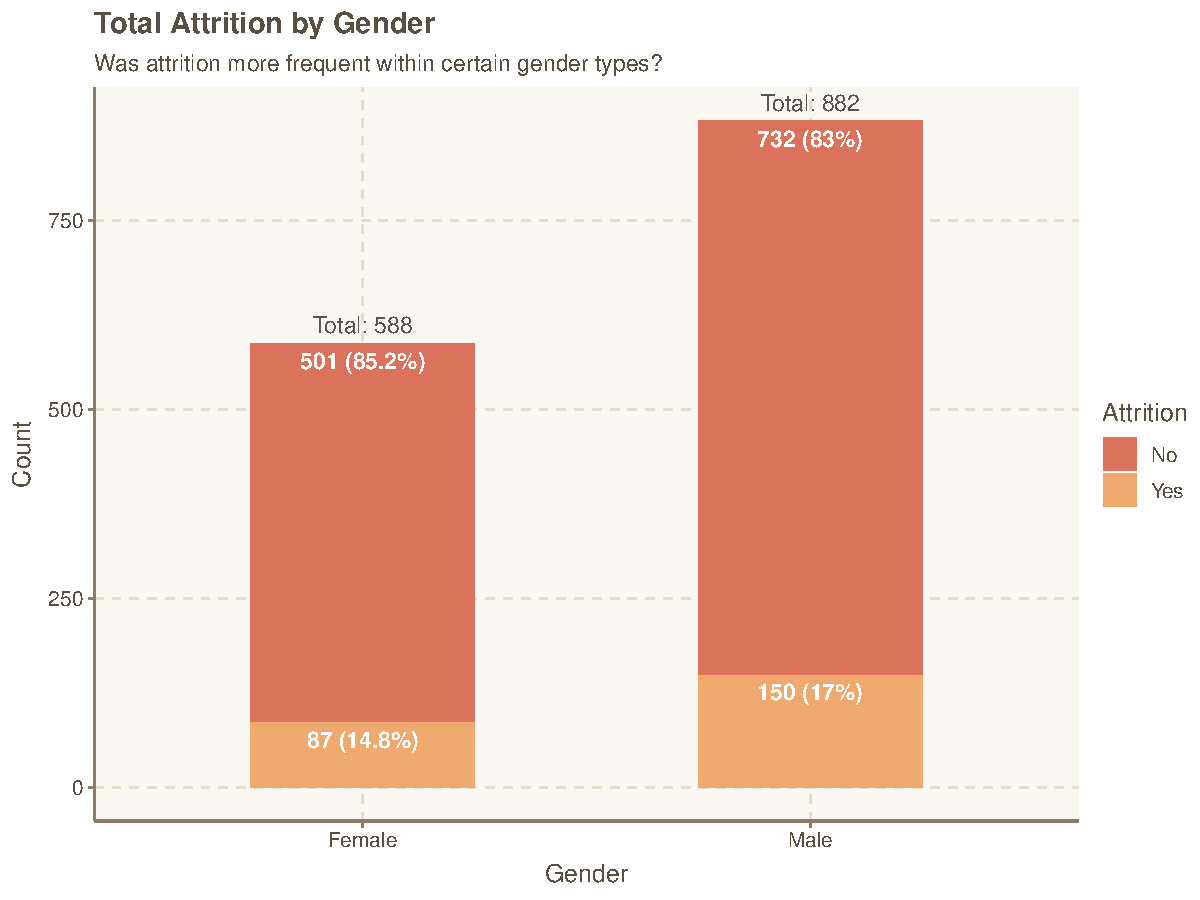
\includegraphics{figures/Gender Attrition Distribubtion-1.pdf}

\begin{itemize}
\item
  \textbf{Quick Takeaways:}

  \begin{itemize}
  \tightlist
  \item
    There are 882 male employees to 588 female employees
  \item
    There was a lower percentage of females leaving the organization
    than males.
  \end{itemize}
\end{itemize}

\begin{Shaded}
\begin{Highlighting}[]
\NormalTok{f_data }\OperatorTok
\StringTok{  }\KeywordTok{ggplot}\NormalTok{(}\KeywordTok{aes}\NormalTok{(}\DataTypeTok{x =}\NormalTok{ Gender,  }\DataTypeTok{fill =}\NormalTok{ Attrition)) }\OperatorTok{+}\StringTok{ }
\StringTok{  }\KeywordTok{geom_bar}\NormalTok{()  }\OperatorTok{+}
\StringTok{  }\KeywordTok{facet_wrap}\NormalTok{(}\KeywordTok{vars}\NormalTok{(JobRole)) }\OperatorTok{+}
\StringTok{  }\KeywordTok{labs}\NormalTok{(}\DataTypeTok{title =} \StringTok{"Attrition by Gender & Job Role"}\NormalTok{,  }
    \DataTypeTok{subtitle =} \StringTok{"Are there attribution differences between genders in certain job roles?"}\NormalTok{)}
\end{Highlighting}
\end{Shaded}

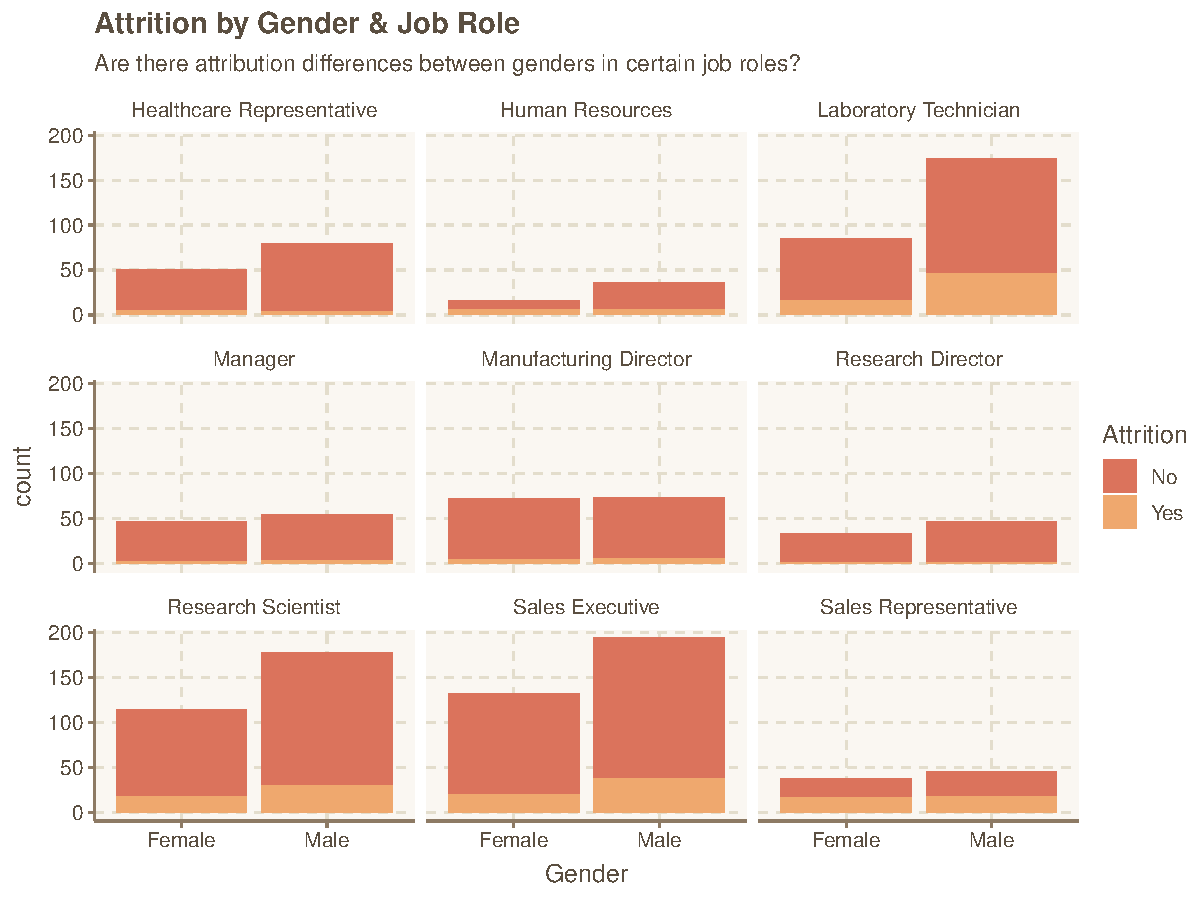
\includegraphics{figures/Gender + Job Role-1.pdf}

\textbf{Quick Takeaways:}

\begin{itemize}
\tightlist
\item
  Overall, relatively proportional attrition between genders with all
  the job role.
\end{itemize}

\begin{Shaded}
\begin{Highlighting}[]
\NormalTok{f_data }\OperatorTok
\StringTok{  }\KeywordTok{ggplot}\NormalTok{(}\KeywordTok{aes}\NormalTok{(}\DataTypeTok{x =}\NormalTok{ Gender,  }\DataTypeTok{fill =}\NormalTok{ Attrition)) }\OperatorTok{+}\StringTok{ }
\StringTok{  }\KeywordTok{geom_bar}\NormalTok{()  }\OperatorTok{+}
\StringTok{  }\KeywordTok{facet_wrap}\NormalTok{(}\KeywordTok{vars}\NormalTok{(JobLevel)) }\OperatorTok{+}
\StringTok{  }\KeywordTok{labs}\NormalTok{(}\DataTypeTok{title =} \StringTok{"Attrition by Gender & Job Level"}\NormalTok{,  }
    \DataTypeTok{subtitle =} \StringTok{"Are there attribution differences between genders in certain job levels?"}\NormalTok{)}
\end{Highlighting}
\end{Shaded}

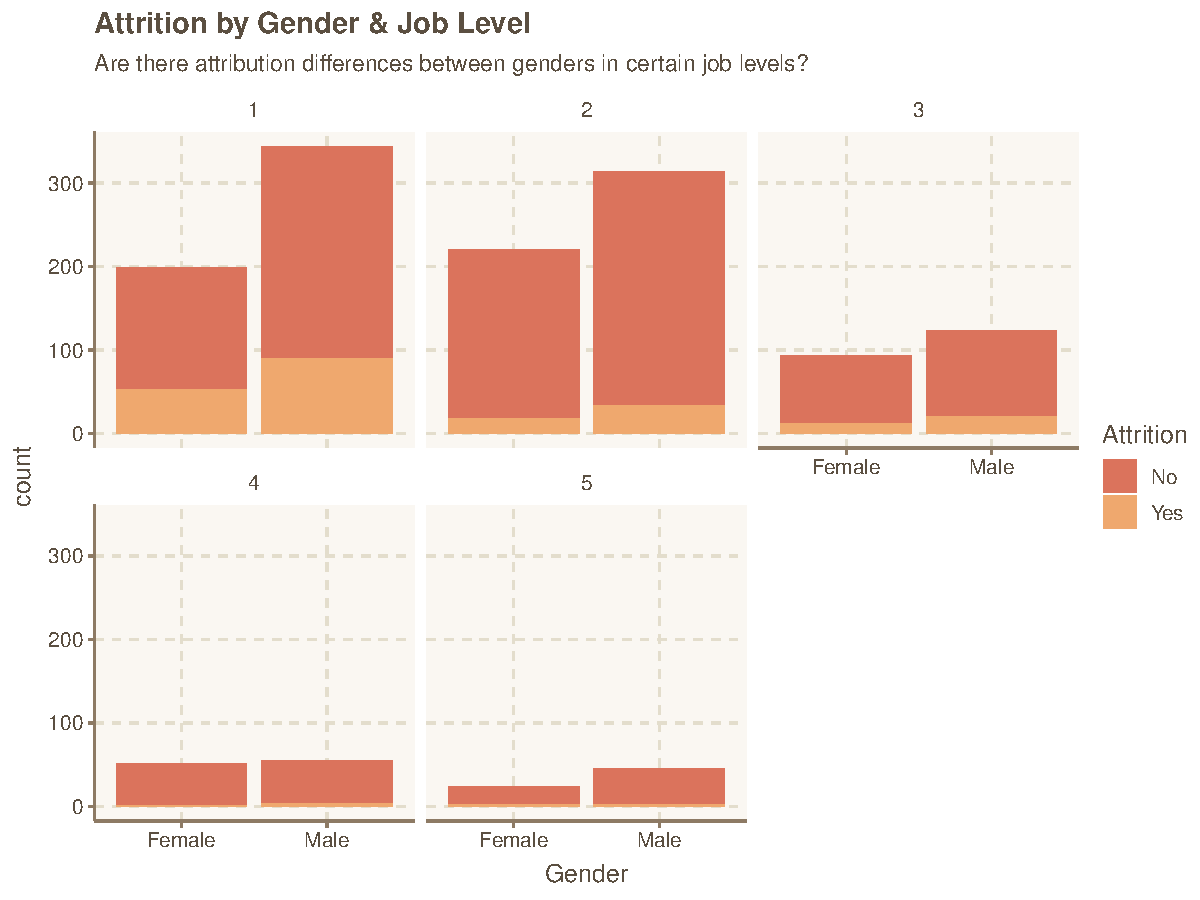
\includegraphics{figures/Gender and Job Level-1.pdf}

\textbf{Quick Takeaways:}

\begin{itemize}
\tightlist
\item
  Overall, the attrition rate between gender seem relatively well
  distributed between job levels.
\end{itemize}

~ ~

\hypertarget{potential-factor-income-differences}{%
\subsection{Potential Factor: Income
Differences}\label{potential-factor-income-differences}}

\textbf{Hypotheses to Test:}

\begin{enumerate}
\def\labelenumi{\arabic{enumi}.}
\tightlist
\item
  Individuals are leaving the organization due to low income.
\item
  Individuals are leaving the organization due to low income in
  comparison to their peers within their job role, department, or level.
  This may be caused by a low perception of organizational fairness.
\item
  Individuals who earn more are more satisfied with their jobs.
\end{enumerate}

\textbf{Summary:}

\begin{enumerate}
\def\labelenumi{\arabic{enumi}.}
\tightlist
\item
  After comparing the income of those who stayed and those who left,
  \textbf{there seems to be support to claim that individuals are
  leaving due to low income.} The median monthly income of all those who
  stayed was 5204 while the median monthly income of those who left was
  3202.
\item
  \textbf{The first point is further supported when analyzing income
  between job roles.} Sales reps, research scientists, and laboratory
  technicians have the lowest income. These roles also have the highest
  attrition rates at 40\%, 24\%, and 16\%. This shows that attrition may
  be correlated with low income.
\item
  \textbf{When looking within job roles and job levels, there was less
  conclusive support that individuals were leaving due to income
  disparities among their peers.} Although income disparities between ex
  and current employees within departments were high, the effect was
  most likely driven by income differences between job roles.
\item
  \textbf{Income does not seem to be a strong driver of job
  satisfaction.}
\end{enumerate}

\textbf{Final thoughts:} The analysis has shown that \textbf{income
seems to be a strong driver of attrition especially for low paying job
roles.} Sales, which had the highest attrition rate was one of the least
paid jobs. The analysis has also shown that \textbf{income disparities
between peers is most likely not a primary reason for attrition.} It may
be relevant to see if job roles such as sales reps, research scientists
and laboratory technicians should have their income levels be
reevaluated and readjusted based on industry and location standards.

\hypertarget{supporting-analysis-for-income-difference}{%
\subsubsection{Supporting Analysis For Income
Difference}\label{supporting-analysis-for-income-difference}}

\textbf{Monthly Income and Attrition}

\begin{Shaded}
\begin{Highlighting}[]
\KeywordTok{ggthemr}\NormalTok{(}\StringTok{'dust'}\NormalTok{)}

\NormalTok{medianvalues <-}\StringTok{ }\NormalTok{f_data }\OperatorTok
\StringTok{  }\KeywordTok{group_by}\NormalTok{(Attrition) }\OperatorTok
\StringTok{  }\KeywordTok{mutate}\NormalTok{(}\DataTypeTok{medians =} \KeywordTok{median}\NormalTok{(MonthlyIncome))}

\NormalTok{f_data }\OperatorTok
\StringTok{  }\KeywordTok{ggplot}\NormalTok{(}\KeywordTok{aes}\NormalTok{(}\DataTypeTok{x =}\NormalTok{ Attrition, }\DataTypeTok{y =}\NormalTok{ MonthlyIncome)) }\OperatorTok{+}\StringTok{ }
\StringTok{  }\KeywordTok{geom_boxplot}\NormalTok{(}\KeywordTok{aes}\NormalTok{(}\DataTypeTok{fill =}\NormalTok{ Attrition)) }\OperatorTok{+}
\StringTok{  }\KeywordTok{geom_text}\NormalTok{(}\DataTypeTok{data =}\NormalTok{ medianvalues, }\KeywordTok{aes}\NormalTok{(}\DataTypeTok{x =}\NormalTok{ Attrition, }\DataTypeTok{y =}\NormalTok{ medians, }\DataTypeTok{label =}\NormalTok{ medians),}
    \DataTypeTok{color =} \StringTok{"white"}\NormalTok{, }\DataTypeTok{fontface =} \StringTok{"bold"}\NormalTok{,}
    \DataTypeTok{vjust =} \DecValTok{-1}\NormalTok{) }\OperatorTok{+}
\StringTok{  }\KeywordTok{labs}\NormalTok{( }\DataTypeTok{x =} \StringTok{"Attrition"}\NormalTok{, }\DataTypeTok{y =} \StringTok{"Monthly Income"}\NormalTok{, }\DataTypeTok{title =} \StringTok{"Attribution by Income"}\NormalTok{, }\DataTypeTok{subtitle =} \StringTok{"Can making less money lead to attrition?"}\NormalTok{)}
\end{Highlighting}
\end{Shaded}

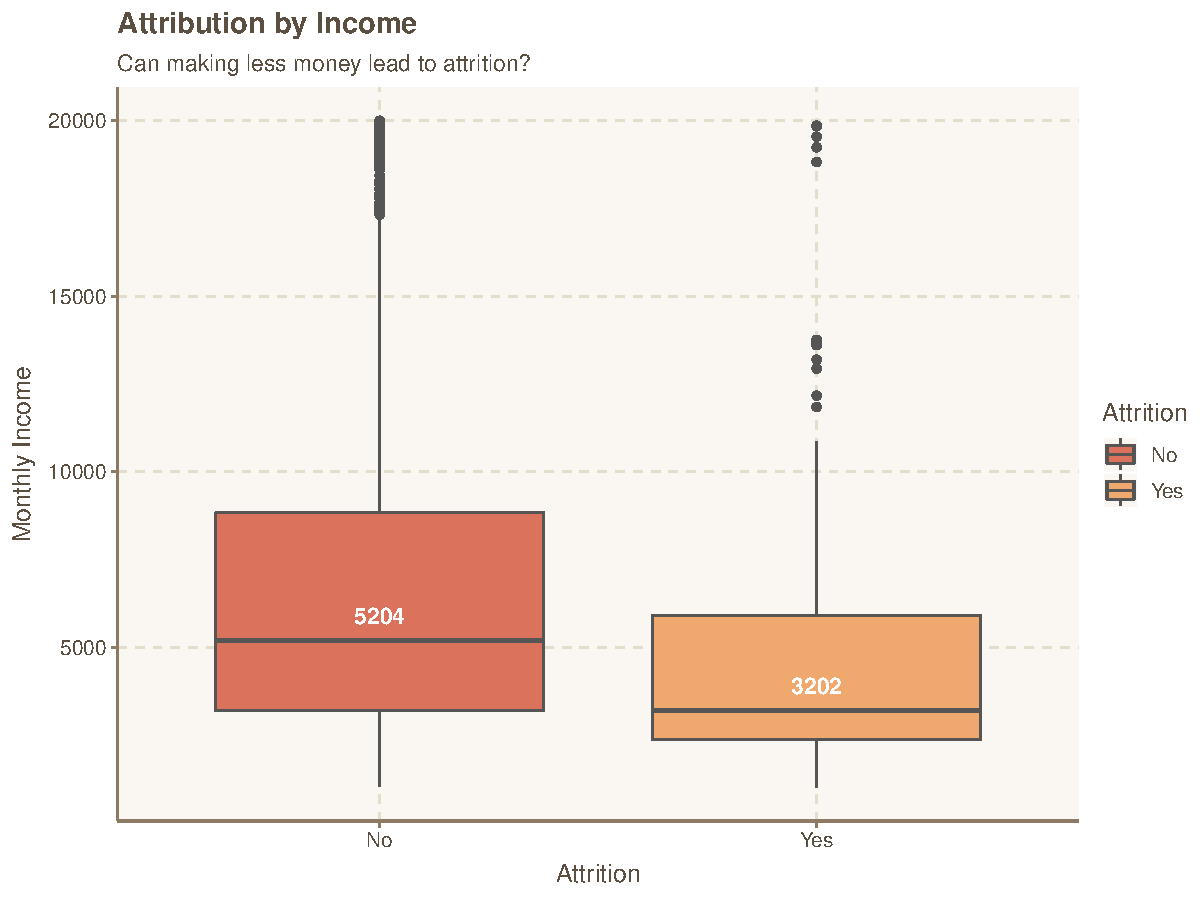
\includegraphics{figures/unnamed-chunk-12-1.pdf}

\textbf{Quick Takeaways:}

\begin{itemize}
\tightlist
\item
  There is a noticeable income difference between people who stayed
  (median = 5204) and left (median = 3202).
\end{itemize}

\textbf{Income by Job Role}

\begin{Shaded}
\begin{Highlighting}[]
\KeywordTok{ggthemr_reset}\NormalTok{()}
\NormalTok{f_data }\OperatorTok
\StringTok{  }\KeywordTok{ggplot}\NormalTok{(}\KeywordTok{aes}\NormalTok{(}\DataTypeTok{x =}\NormalTok{ Age , }\DataTypeTok{y =}\NormalTok{ MonthlyIncome, }\DataTypeTok{col =}\NormalTok{ JobRole)) }\OperatorTok{+}\StringTok{ }
\StringTok{  }\KeywordTok{geom_point}\NormalTok{() }\OperatorTok{+}\StringTok{ }
\StringTok{  }\KeywordTok{geom_smooth}\NormalTok{(}\DataTypeTok{method =} \StringTok{"lm"}\NormalTok{, }\DataTypeTok{se =} \OtherTok{FALSE}\NormalTok{) }\OperatorTok{+}
\StringTok{  }\KeywordTok{labs}\NormalTok{(}\DataTypeTok{title =} \StringTok{"Income by Job Role"}\NormalTok{, }\DataTypeTok{subtitle =} \StringTok{"How much money are people making within each job role?"}\NormalTok{) }\OperatorTok{+}\StringTok{ }
\StringTok{  }\KeywordTok{scale_y_continuous}\NormalTok{(}\DataTypeTok{breaks =} \KeywordTok{seq}\NormalTok{(}\DecValTok{0}\NormalTok{, }\DecValTok{20000}\NormalTok{, }\DecValTok{5000}\NormalTok{),}
                      \DataTypeTok{labels =} \KeywordTok{paste0}\NormalTok{(}\KeywordTok{as.character}\NormalTok{(}\KeywordTok{seq}\NormalTok{(}\DecValTok{0}\NormalTok{,}\DecValTok{20}\NormalTok{,}\DecValTok{5}\NormalTok{)),}\StringTok{"K"}\NormalTok{)) }\OperatorTok{+}
\StringTok{  }\KeywordTok{facet_wrap}\NormalTok{(}\KeywordTok{vars}\NormalTok{(JobRole)) }\OperatorTok{+}\StringTok{ }
\StringTok{  }\KeywordTok{theme_minimal}\NormalTok{() }\OperatorTok{+}\StringTok{ }
\StringTok{  }\KeywordTok{theme}\NormalTok{(}\DataTypeTok{text =} \KeywordTok{element_text}\NormalTok{( }\DataTypeTok{color =} \StringTok{'#5b4f41'}\NormalTok{), }
    \DataTypeTok{plot.title =} \KeywordTok{element_text}\NormalTok{(}\DataTypeTok{size =} \DecValTok{16}\NormalTok{, }\DataTypeTok{face =} \StringTok{"bold"}\NormalTok{),}
    \DataTypeTok{panel.background =} \KeywordTok{element_rect}\NormalTok{(}\DataTypeTok{fill =} \StringTok{"#FAF7F2"}\NormalTok{),}
    \DataTypeTok{panel.grid.major =} \KeywordTok{element_line}\NormalTok{(}\DataTypeTok{colour =} \StringTok{"#E3DDCC"}\NormalTok{))}
\end{Highlighting}
\end{Shaded}

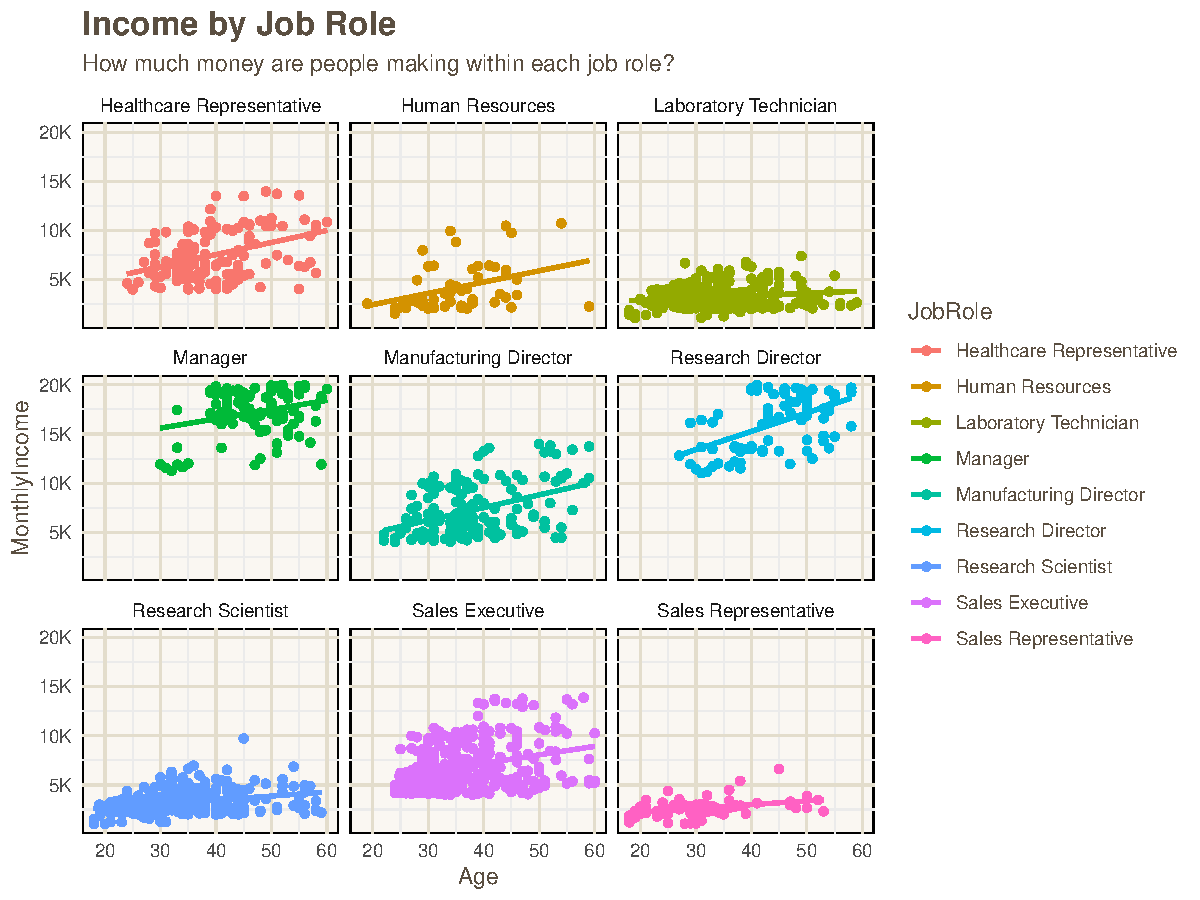
\includegraphics{figures/Income by Job Role-1.pdf}

\textbf{Quick Takeaways:}

\begin{itemize}
\tightlist
\item
  Managers and Research Directors make the most income. The two
  positions also have the lowest attrition rate at 5\% and 3\%
  respectively.
\item
  Sales reps, laboratory technicians, and research scientists have the
  lowest income. These three positions have high attrition rates at
  40\%, 24\%, and 16\% each.
\item
  This seems to support my hypothesis that lower income leads to
\end{itemize}

\textbf{Income Differences by Job Role and Attrition}

\begin{Shaded}
\begin{Highlighting}[]
\KeywordTok{ggthemr}\NormalTok{(}\StringTok{'dust'}\NormalTok{)}
\NormalTok{f_data }\OperatorTok
\StringTok{  }\KeywordTok{mutate}\NormalTok{(}\DataTypeTok{JobRole =} \KeywordTok{gsub}\NormalTok{(}\StringTok{" "}\NormalTok{, }\StringTok{"}\CharTok{\textbackslash{}n}\StringTok{"}\NormalTok{, JobRole)) }\OperatorTok
\StringTok{  }\KeywordTok{ggplot}\NormalTok{(}\KeywordTok{aes}\NormalTok{(}\DataTypeTok{x =}\NormalTok{ JobRole, }\DataTypeTok{y =}\NormalTok{ MonthlyIncome, }\DataTypeTok{fill =}\NormalTok{ Attrition)) }\OperatorTok{+}\StringTok{ }
\StringTok{  }\KeywordTok{geom_boxplot}\NormalTok{() }\OperatorTok{+}\StringTok{ }
\StringTok{  }\KeywordTok{theme}\NormalTok{(}\DataTypeTok{legend.position =} \StringTok{"top"}\NormalTok{) }\OperatorTok{+}
\StringTok{  }\KeywordTok{labs}\NormalTok{( }\DataTypeTok{x =} \StringTok{"Job Role"}\NormalTok{, }\DataTypeTok{y =} \StringTok{"Monthly Income"}\NormalTok{, }\DataTypeTok{title =} \StringTok{"Income by Job Role and Attrition"}\NormalTok{, }\DataTypeTok{subtitle =} \StringTok{"Are people leaving because they are making less than their coworkers in the same role?"}\NormalTok{)}
\end{Highlighting}
\end{Shaded}

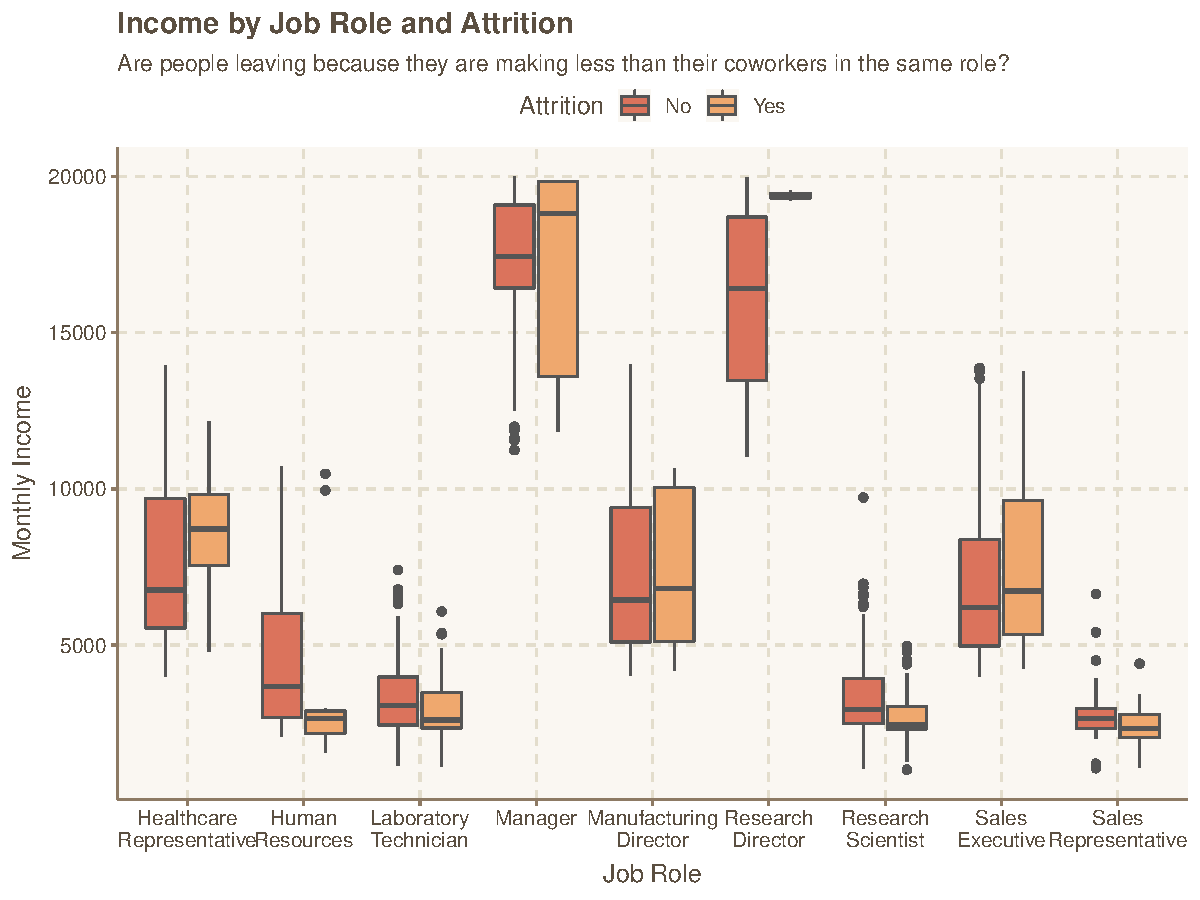
\includegraphics{figures/Income Differences by Job Role and Attrition-1.pdf}

\textbf{Quick Takeaways:}

\begin{itemize}
\tightlist
\item
  Overall, there does not seem to be strong evidence supporting the
  claim that people are leaving due to income differences within roles.
\item
  In fact, there are many instances (healthcare reps, managers,
  manufacturing director, research director, and sales executives) where
  the attrition group has a higher median income than the group that
  stayed.
\end{itemize}

\textbf{Income Differences by Department and Attrition}

\begin{Shaded}
\begin{Highlighting}[]
\KeywordTok{ggthemr}\NormalTok{(}\StringTok{'dust'}\NormalTok{)}
\NormalTok{f_data }\OperatorTok
\StringTok{  }\KeywordTok{ggplot}\NormalTok{(}\KeywordTok{aes}\NormalTok{(}\DataTypeTok{x =}\NormalTok{ Department, }\DataTypeTok{y =}\NormalTok{ MonthlyIncome, }\DataTypeTok{fill =}\NormalTok{ Attrition)) }\OperatorTok{+}\StringTok{ }
\StringTok{  }\KeywordTok{geom_boxplot}\NormalTok{() }\OperatorTok{+}\StringTok{ }
\StringTok{  }\KeywordTok{theme}\NormalTok{(}\DataTypeTok{legend.position =} \StringTok{"top"}\NormalTok{) }\OperatorTok{+}
\StringTok{  }\KeywordTok{labs}\NormalTok{( }\DataTypeTok{x =} \StringTok{"Department"}\NormalTok{, }\DataTypeTok{y =} \StringTok{"Monthly Income"}\NormalTok{, }\DataTypeTok{title =} \StringTok{"Income by Department"}\NormalTok{, }\DataTypeTok{subtitle =} \StringTok{"Can making less money among peers within departments lead to attrition?"}\NormalTok{ )}
\end{Highlighting}
\end{Shaded}

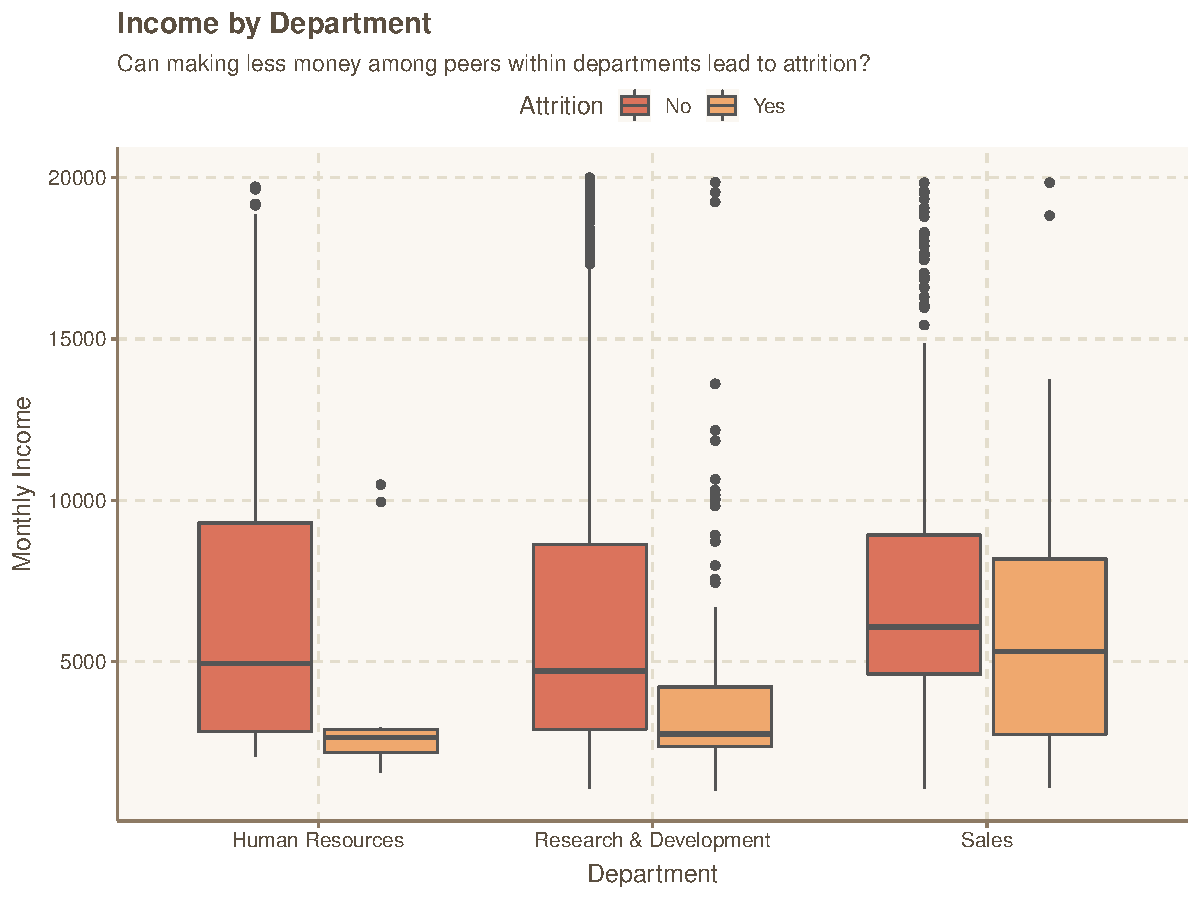
\includegraphics{figures/Income Differences by Department and Attrition-1.pdf}

\textbf{Quick Takeaways:}

\begin{itemize}
\tightlist
\item
  Although there was no strong support for attrition due income
  differences within job roles, there does seem to be support when it
  comes to departments.
\item
  This leads me to hypothesize that the problem exists within
  departments rather than job roles. For example, research scientists
  who make far less than research directors are more likely to leave due
  to the income disparity between the two roles.
\end{itemize}

\textbf{Income Differences by Job Level and Attrition}

\begin{Shaded}
\begin{Highlighting}[]
\KeywordTok{ggthemr}\NormalTok{(}\StringTok{'dust'}\NormalTok{)}
\NormalTok{f_data }\OperatorTok
\StringTok{  }\KeywordTok{ggplot}\NormalTok{(}\KeywordTok{aes}\NormalTok{(}\DataTypeTok{x =} \KeywordTok{as.factor}\NormalTok{(JobLevel), }\DataTypeTok{y =}\NormalTok{ MonthlyIncome, }\DataTypeTok{fill =}\NormalTok{ Attrition)) }\OperatorTok{+}\StringTok{ }
\StringTok{  }\KeywordTok{geom_boxplot}\NormalTok{() }\OperatorTok{+}\StringTok{ }
\StringTok{  }\KeywordTok{theme}\NormalTok{(}\DataTypeTok{legend.position =} \StringTok{"top"}\NormalTok{) }\OperatorTok{+}
\StringTok{  }\KeywordTok{labs}\NormalTok{( }\DataTypeTok{x =} \StringTok{"Job Level"}\NormalTok{, }\DataTypeTok{y =} \StringTok{"Monthly Income"}\NormalTok{,}
    \DataTypeTok{title =} \StringTok{"Income by Job Level and Attrition"}\NormalTok{, }
    \DataTypeTok{subtitle =} \StringTok{"Can making less money among peers within the same job level lead to attrition?"}\NormalTok{ )}
\end{Highlighting}
\end{Shaded}

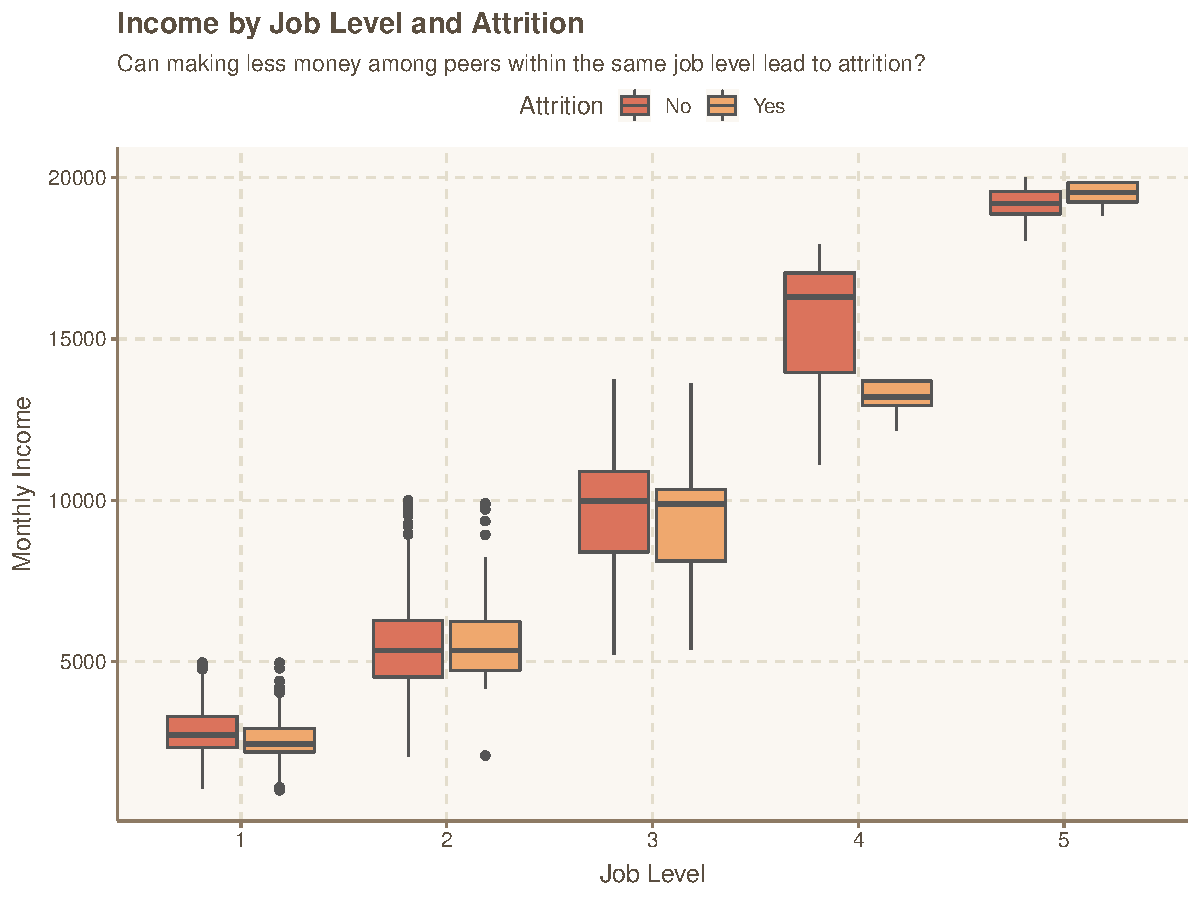
\includegraphics{figures/Income Differences by Job Level and Attrition-1.pdf}

\textbf{Quick Takeaways:}

\begin{itemize}
\tightlist
\item
  Overall, there does not seem to be strong support for attrition due to
  income differences within job levels.
\item
  The only level where huge income differences occurred was in level 4.
  Further analysis on level 4 may be required.
\end{itemize}

\textbf{Income Differences by Job Satisfaction and Attrition}

\begin{Shaded}
\begin{Highlighting}[]
\KeywordTok{ggthemr}\NormalTok{(}\StringTok{'dust'}\NormalTok{)}
\NormalTok{f_data }\OperatorTok
\StringTok{  }\KeywordTok{group_by}\NormalTok{(JobSatisfaction, Attrition) }\OperatorTok
\StringTok{  }\KeywordTok{summarise}\NormalTok{(}\DataTypeTok{AvgInc =} \KeywordTok{mean}\NormalTok{(MonthlyIncome)) }\OperatorTok
\StringTok{  }\KeywordTok{mutate}\NormalTok{(}\DataTypeTok{JobSatisfaction =} \KeywordTok{gsub}\NormalTok{(}\StringTok{"^"}\NormalTok{, }\StringTok{"Satisfaction }\CharTok{\textbackslash{}n}\StringTok{ Level "}\NormalTok{, JobSatisfaction)) }\OperatorTok
\StringTok{  }\KeywordTok{ggplot}\NormalTok{(}\KeywordTok{aes}\NormalTok{(}\DataTypeTok{x =}\NormalTok{ JobSatisfaction, }\DataTypeTok{y =}\NormalTok{ AvgInc)) }\OperatorTok{+}
\StringTok{  }\KeywordTok{geom_point}\NormalTok{(}\DataTypeTok{size =} \DecValTok{5}\NormalTok{, }\KeywordTok{aes}\NormalTok{(}\DataTypeTok{y =}\NormalTok{ AvgInc, }\DataTypeTok{color =}\NormalTok{ Attrition)) }\OperatorTok{+}
\StringTok{  }\KeywordTok{geom_segment}\NormalTok{(}\KeywordTok{aes}\NormalTok{(}\DataTypeTok{x =}\NormalTok{ JobSatisfaction, }\DataTypeTok{xend =}\NormalTok{ JobSatisfaction, }\DataTypeTok{y =} \DecValTok{0}\NormalTok{, }
    \DataTypeTok{yend =}\NormalTok{ AvgInc, }\DataTypeTok{color =}\NormalTok{ Attrition), }\DataTypeTok{size =} \FloatTok{1.2}\NormalTok{, }\DataTypeTok{linetype =} \DecValTok{1}\NormalTok{, }\DataTypeTok{alpha =} \FloatTok{.8}\NormalTok{) }\OperatorTok{+}
\StringTok{  }\KeywordTok{facet_wrap}\NormalTok{(}\KeywordTok{vars}\NormalTok{(Attrition))}\OperatorTok{+}\StringTok{ }
\StringTok{  }\KeywordTok{scale_y_continuous}\NormalTok{(}\DataTypeTok{limits =} \KeywordTok{c}\NormalTok{(}\DecValTok{0}\NormalTok{,}\DecValTok{8000}\NormalTok{)) }\OperatorTok{+}
\StringTok{  }\KeywordTok{labs}\NormalTok{(}\DataTypeTok{x =} \StringTok{"Job Satisfaction Levels"}\NormalTok{, }\DataTypeTok{y =} \StringTok{"Average Income"}\NormalTok{, }
    \DataTypeTok{title =} \StringTok{"Average Income by Satisfaction Level and Attrition"}\NormalTok{, }
    \DataTypeTok{subtitle =} \StringTok{"Are people leaving because they are unsatisfied due to their low income?"}\NormalTok{) }\OperatorTok{+}\StringTok{ }
\StringTok{  }\KeywordTok{geom_text}\NormalTok{(}\KeywordTok{aes}\NormalTok{(}\DataTypeTok{x =}\NormalTok{ JobSatisfaction, }\DataTypeTok{y =}\NormalTok{ AvgInc,}
    \DataTypeTok{label =} \KeywordTok{round}\NormalTok{(AvgInc,}\DecValTok{0}\NormalTok{)), }\DataTypeTok{vjust =} \DecValTok{-1}\NormalTok{) }\OperatorTok{+}
\StringTok{  }\KeywordTok{scale_color_ggthemr_d}\NormalTok{() }\OperatorTok{+}
\StringTok{  }\KeywordTok{theme}\NormalTok{(}\DataTypeTok{strip.text.x =} \KeywordTok{element_blank}\NormalTok{(), }\DataTypeTok{legend.position =} \StringTok{"top"}\NormalTok{)}
\end{Highlighting}
\end{Shaded}

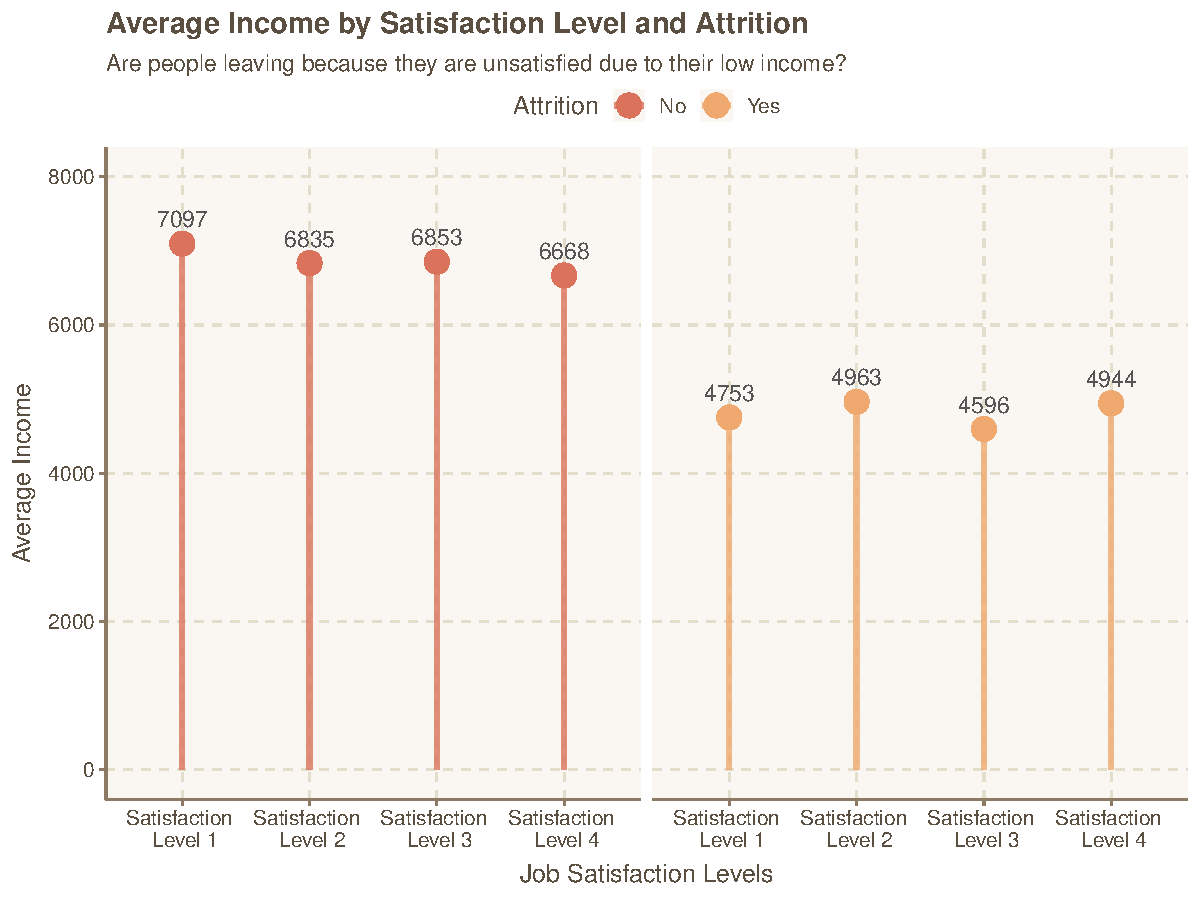
\includegraphics{figures/unnamed-chunk-13-1.pdf}

\textbf{Quick Takeaways:}

\begin{itemize}
\tightlist
\item
  Overall, there doesn't seem to be strong support showing that lower
  income is the reason for lower job satisfaction. For those who left
  and those who stayed, average income did not rise with rising job
  satisfaction. In fact, there is nearly 0 correlation between income
  and job satisfaction.
\end{itemize}

~ ~

\hypertarget{potential-factor-satisfaction-variables}{%
\subsection{Potential Factor: Satisfaction
Variables}\label{potential-factor-satisfaction-variables}}

\textbf{Hypotheses to Test:}

\begin{enumerate}
\def\labelenumi{\arabic{enumi}.}
\tightlist
\item
  Individuals are leaving the organization due to low levels of job
  satisfaction
\item
  Individuals are leaving the organization due to levels of
  environmental satisfaction
\item
  Individuals are leaving the organization due to working overtime.
\end{enumerate}

\textbf{Summary:}

\begin{enumerate}
\def\labelenumi{\arabic{enumi}.}
\tightlist
\item
  After comparing the average job satisfaction by role and attrition, it
  is evident that for the jobs with the highest attrition rates
  (e.g.~sales rep, lab tech, and human resources), there was a large gap
  in average job satisfaction for those who left and those who stayed.
\item
  This effect however is close to 0 for manufactoring director and
  healthcare representative.
\item
  After comparing the average environment satisfaction by role and
  attrition, healthcare representative and managers (two job roles that
  does not have high attrition rates) have the largest gaps between
  those who leave and those who stay. Understanding their environment
  and how their environment is affecting their work will be critical.
\item
  In addition, exploratory data analysis shows that that for sales reps
  and research scientists, the average environmental satisfaction gap
  between those who stayed and those who left were minimal. This
  indicates that for those roles, environment did not play a huge factor
  in determining leaving the organization.
\item
  30.5\% of individuals who worked overtime left the organization in
  comparison to 10.4\% of individuals who did not.
\item
  However, overtime was relatively constant throughout levels and job
  role. It may be worth considering other factors that contribute to
  when and which employees work overtime.
\item
  Overtime did not seem to be a driver of job satisfaction and
  environment satisfaciton
\end{enumerate}

\textbf{Final thoughts:}

There is strong evidence that factors relating to satisfaction are key
drivers to attrition. Job satisfaction seems to be a bigger factor for
roles with high levels of attrition such as Sales Rep, Laboratory
technicians, human resources, and sales executives. However environment
satisfaction seems to be a bigger factor for roles with low attrition
such as Healthcare reps, and managers. Managers seem to be the most
impacted by ow Environment Satisfaction. Overtime also seems to play a
factor in attrition. However, overtime rates seem relatively similar
within roles and level.

~ ~

\hypertarget{supporting-analysis-for-satisfaction-differences}{%
\subsubsection{Supporting Analysis for Satisfaction
Differences}\label{supporting-analysis-for-satisfaction-differences}}

\textbf{Job Satisfaction by Job Roles and Attrition (ordered by highest
to lowest attrition rate)}

\begin{Shaded}
\begin{Highlighting}[]
\KeywordTok{ggthemr}\NormalTok{(}\StringTok{'fresh'}\NormalTok{)}
\NormalTok{f_data }\OperatorTok\StringTok{ }
\StringTok{  }\KeywordTok{select}\NormalTok{(JobRole, JobSatisfaction, Attrition) }\OperatorTok
\StringTok{  }\KeywordTok{group_by}\NormalTok{(JobRole, Attrition) }\OperatorTok
\StringTok{  }\KeywordTok{summarise}\NormalTok{(}\DataTypeTok{avg =} \KeywordTok{mean}\NormalTok{(JobSatisfaction)) }\OperatorTok
\StringTok{  }\KeywordTok{mutate}\NormalTok{(}\DataTypeTok{JobRole =} \KeywordTok{gsub}\NormalTok{(}\StringTok{" "}\NormalTok{, }\StringTok{"}\CharTok{\textbackslash{}n}\StringTok{"}\NormalTok{, JobRole)) }\OperatorTok
\StringTok{  }\KeywordTok{mutate}\NormalTok{(}\DataTypeTok{JobRole =} \KeywordTok{as.factor}\NormalTok{(JobRole)) }\OperatorTok
\StringTok{  }\KeywordTok{mutate}\NormalTok{(}\DataTypeTok{JobRole =} \KeywordTok{fct_relevel}\NormalTok{(JobRole, }\StringTok{"Sales}\CharTok{\textbackslash{}n}\StringTok{Representative"}\NormalTok{, }\StringTok{"Laboratory}\CharTok{\textbackslash{}n}\StringTok{Technician"}\NormalTok{, }
    \StringTok{"Human}\CharTok{\textbackslash{}n}\StringTok{Resources"}\NormalTok{, }\StringTok{"Sales}\CharTok{\textbackslash{}n}\StringTok{Executive"}\NormalTok{,}
    \StringTok{"Research}\CharTok{\textbackslash{}n}\StringTok{Scientist"}\NormalTok{, }\StringTok{"Manufacturing}\CharTok{\textbackslash{}n}\StringTok{Director"}\NormalTok{,}
    \StringTok{"Healthcare}\CharTok{\textbackslash{}n}\StringTok{Representative"}\NormalTok{, }\StringTok{"Manager"}\NormalTok{,}
    \StringTok{"Research}\CharTok{\textbackslash{}n}\StringTok{Director"}\NormalTok{)) }\OperatorTok
\StringTok{  }\KeywordTok{ggplot}\NormalTok{(}\KeywordTok{aes}\NormalTok{(}\DataTypeTok{x =}\NormalTok{ JobRole, }\DataTypeTok{y =}\NormalTok{ avg, }\DataTypeTok{color =}\NormalTok{ Attrition)) }\OperatorTok{+}
\StringTok{  }\KeywordTok{geom_point}\NormalTok{(}\DataTypeTok{size =} \DecValTok{4}\NormalTok{) }\OperatorTok{+}\StringTok{ }
\StringTok{  }\KeywordTok{geom_line}\NormalTok{(}\KeywordTok{aes}\NormalTok{(}\DataTypeTok{group =}\NormalTok{ Attrition), }\DataTypeTok{linetype =} \StringTok{"dashed"}\NormalTok{) }\OperatorTok{+}
\StringTok{  }\KeywordTok{labs}\NormalTok{(}\DataTypeTok{title =} \StringTok{"Average Job Satisfaction by Job Role & Attrition"}\NormalTok{,}
    \DataTypeTok{subtitle =} \StringTok{"Are people leaving due to low job satisfaction?"}\NormalTok{,}
    \DataTypeTok{x =} \StringTok{"Job Roles (ordered from highest to lowest attrition rate)"}\NormalTok{,}
    \DataTypeTok{y =} \StringTok{"Average Job Satisfaction"}\NormalTok{) }\OperatorTok{+}
\StringTok{  }\KeywordTok{scale_color_ggthemr_d}\NormalTok{() }\OperatorTok{+}
\StringTok{  }\KeywordTok{theme}\NormalTok{(}\DataTypeTok{legend.position =} \StringTok{'top'}\NormalTok{)}
\end{Highlighting}
\end{Shaded}

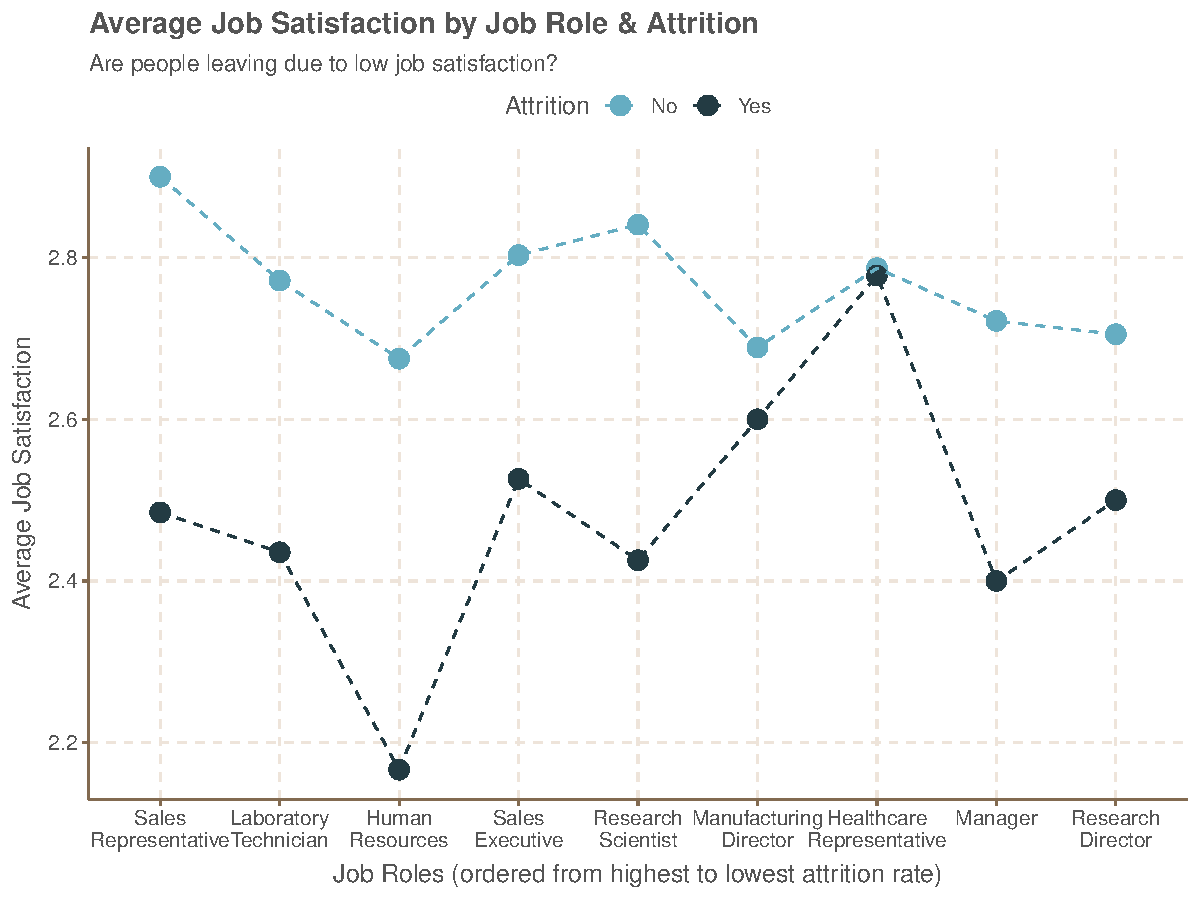
\includegraphics{figures/unnamed-chunk-14-1.pdf}

\textbf{Quick Takeaways:}

\begin{itemize}
\tightlist
\item
  Here we find something really interesting. Overall, those who leave
  the organization tend to have lower job satisfaction ratings.
\item
  However, the effect of job satisfaction on attrition seems to be
  stronger for those who are in job roles with higher attrition rate.
\item
  The difference in job satisfaction is smaller when you go to job roles
  with lower attrition rates.
\end{itemize}

\textbf{Attrition by Environmental Satisfaction}

\begin{Shaded}
\begin{Highlighting}[]
\NormalTok{f_data }\OperatorTok\StringTok{ }
\StringTok{  }\KeywordTok{select}\NormalTok{(JobRole, EnvironmentSatisfaction, Attrition) }\OperatorTok
\StringTok{  }\KeywordTok{group_by}\NormalTok{(JobRole, Attrition) }\OperatorTok
\StringTok{  }\KeywordTok{summarise}\NormalTok{(}\DataTypeTok{avg =} \KeywordTok{mean}\NormalTok{(EnvironmentSatisfaction)) }\OperatorTok
\StringTok{  }\KeywordTok{mutate}\NormalTok{(}\DataTypeTok{JobRole =} \KeywordTok{gsub}\NormalTok{(}\StringTok{" "}\NormalTok{, }\StringTok{"}\CharTok{\textbackslash{}n}\StringTok{"}\NormalTok{, JobRole)) }\OperatorTok
\StringTok{  }\KeywordTok{mutate}\NormalTok{(}\DataTypeTok{JobRole =} \KeywordTok{as.factor}\NormalTok{(JobRole)) }\OperatorTok
\StringTok{  }\KeywordTok{mutate}\NormalTok{(}\DataTypeTok{JobRole =} \KeywordTok{fct_relevel}\NormalTok{(JobRole, }\StringTok{"Sales}\CharTok{\textbackslash{}n}\StringTok{Representative"}\NormalTok{, }\StringTok{"Laboratory}\CharTok{\textbackslash{}n}\StringTok{Technician"}\NormalTok{,}
    \StringTok{"Human}\CharTok{\textbackslash{}n}\StringTok{Resources"}\NormalTok{, }\StringTok{"Sales}\CharTok{\textbackslash{}n}\StringTok{Executive"}\NormalTok{, }
    \StringTok{"Research}\CharTok{\textbackslash{}n}\StringTok{Scientist"}\NormalTok{, }\StringTok{"Manufacturing}\CharTok{\textbackslash{}n}\StringTok{Director"}\NormalTok{,}
    \StringTok{"Healthcare}\CharTok{\textbackslash{}n}\StringTok{Representative"}\NormalTok{, }\StringTok{"Manager"}\NormalTok{,}
    \StringTok{"Research}\CharTok{\textbackslash{}n}\StringTok{Director"}\NormalTok{)) }\OperatorTok
\StringTok{  }\KeywordTok{ggplot}\NormalTok{(}\KeywordTok{aes}\NormalTok{(}\DataTypeTok{x =}\NormalTok{ JobRole, }\DataTypeTok{y =}\NormalTok{ avg, }\DataTypeTok{color =}\NormalTok{ Attrition)) }\OperatorTok{+}
\StringTok{  }\KeywordTok{geom_point}\NormalTok{(}\DataTypeTok{size =} \DecValTok{4}\NormalTok{) }\OperatorTok{+}\StringTok{ }
\StringTok{  }\KeywordTok{geom_line}\NormalTok{(}\KeywordTok{aes}\NormalTok{(}\DataTypeTok{group =}\NormalTok{ Attrition), }\DataTypeTok{linetype =} \StringTok{"dashed"}\NormalTok{) }\OperatorTok{+}
\StringTok{  }\KeywordTok{labs}\NormalTok{(}\DataTypeTok{title =} \StringTok{"Average Environment Satisfaction by Job Role & Attrition"}\NormalTok{,}
    \DataTypeTok{subtitle =} \StringTok{"Are people leaving due to low environment satisfaction?"}\NormalTok{,}
    \DataTypeTok{x =} \StringTok{"Job Roles (ordered from highest to lowest attrition rate)"}\NormalTok{,}
    \DataTypeTok{y =} \StringTok{"Average Environmental Satisfaction"}\NormalTok{) }\OperatorTok{+}
\StringTok{  }\KeywordTok{scale_color_ggthemr_d}\NormalTok{() }\OperatorTok{+}
\StringTok{  }\KeywordTok{theme}\NormalTok{(}\DataTypeTok{legend.position =} \StringTok{"top"}\NormalTok{)}
\end{Highlighting}
\end{Shaded}

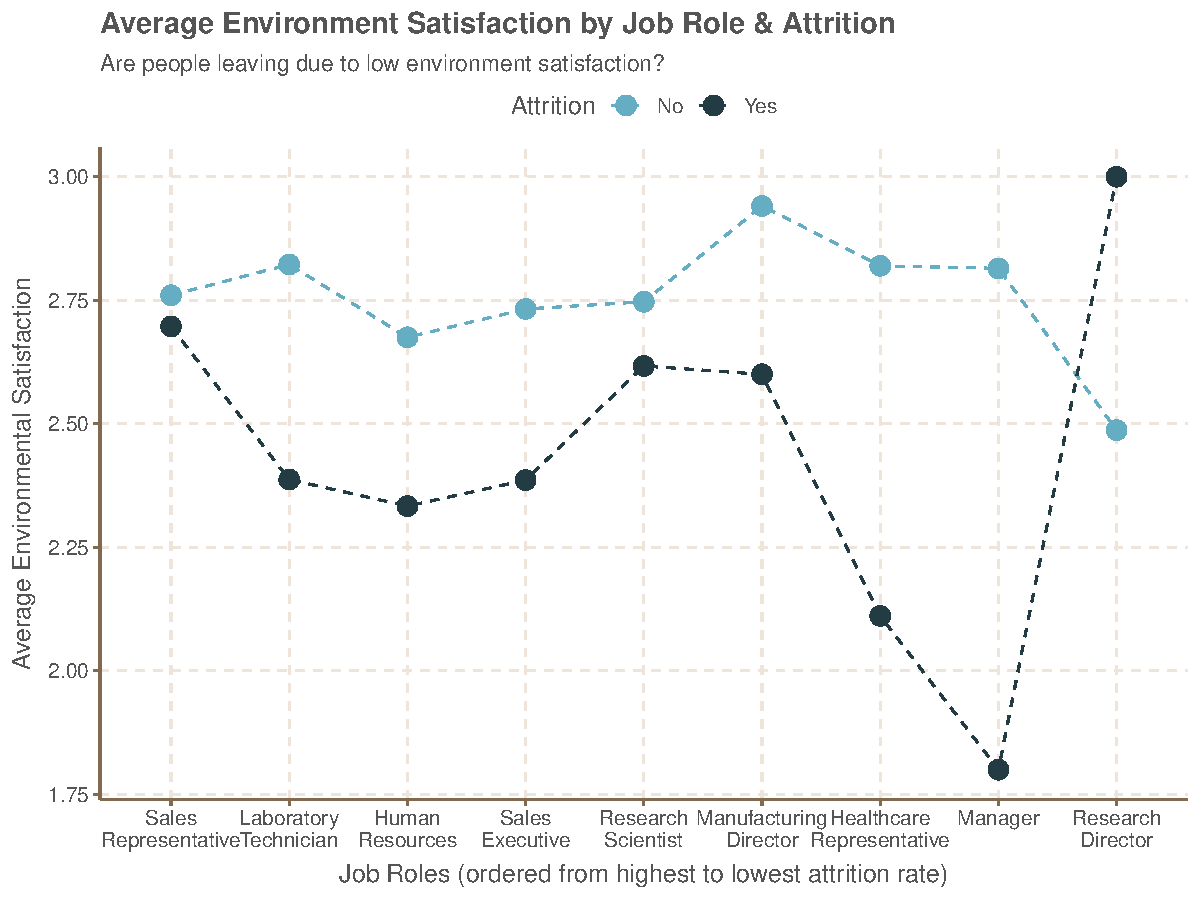
\includegraphics{figures/unnamed-chunk-15-1.pdf}

\textbf{Quick Takeaways:}

\begin{itemize}
\tightlist
\item
  Here we find something really interesting again. Overall, those who
  leave the organization tend to have lower environmental satisfaction
  ratings. This effect however is close to 0 for manufactoring director
  and healthcare representative.
\item
  However, in an opposite trend to job satisfaction, the effect of
  environmental satisfaction ratings on attrition seems higher for job
  roles with higher attrition rates.
\item
  This shows that while job satisfaction may have a stronger role in
  attrition for sales rep, laboratory technician, HR, environmental
  satisfaction may have a stronger role for positions like healthcare
  representative and managers.
\item
  Strangely enough research director was the only position that had
  higher environmental satisfaction for those who left compared to those
  who stayed.
\item
  The largest difference in environment satisfaction ratings were from
  Managers. There should be an investigation to see what is driving such
  low environmental satisfaction from Managers.
\end{itemize}

\textbf{Attrition by Overtime}

\begin{Shaded}
\begin{Highlighting}[]
\KeywordTok{ggthemr}\NormalTok{(}\StringTok{"fresh"}\NormalTok{)}
\NormalTok{f_data }\OperatorTok
\StringTok{  }\KeywordTok{group_by}\NormalTok{(Attrition, OverTime) }\OperatorTok
\StringTok{  }\KeywordTok{summarise}\NormalTok{(}\DataTypeTok{Count =} \KeywordTok{n}\NormalTok{()) }\OperatorTok
\StringTok{  }\KeywordTok{group_by}\NormalTok{(OverTime) }\OperatorTok
\StringTok{  }\KeywordTok{arrange}\NormalTok{(Count) }\OperatorTok
\StringTok{  }\KeywordTok{mutate}\NormalTok{(}\DataTypeTok{Count_total =} \KeywordTok{cumsum}\NormalTok{(Count),}
    \DataTypeTok{CountPer =} \KeywordTok{prop.table}\NormalTok{(Count),}
    \DataTypeTok{final =} \KeywordTok{paste}\NormalTok{(Count, }\StringTok{" ("}\NormalTok{, }\KeywordTok{round}\NormalTok{(CountPer}\OperatorTok{*}\DecValTok{100}\NormalTok{,}\DecValTok{1}\NormalTok{), }\StringTok{"%)"}\NormalTok{, }\DataTypeTok{sep =} \StringTok{""}\NormalTok{),}
    \DataTypeTok{total =} \KeywordTok{paste}\NormalTok{(}\StringTok{"Total:"}\NormalTok{, }\KeywordTok{sum}\NormalTok{(Count)),}
    \DataTypeTok{top =} \KeywordTok{sum}\NormalTok{(Count)) }\OperatorTok
\StringTok{  }\KeywordTok{ggplot}\NormalTok{(}\KeywordTok{aes}\NormalTok{(}\DataTypeTok{x =}\NormalTok{ OverTime, }\DataTypeTok{y =}\NormalTok{ Count, }\DataTypeTok{fill =}\NormalTok{ Attrition)) }\OperatorTok{+}\StringTok{ }
\StringTok{  }\KeywordTok{geom_bar}\NormalTok{(}\DataTypeTok{stat =} \StringTok{"identity"}\NormalTok{, }\DataTypeTok{width =} \FloatTok{.5}\NormalTok{) }\OperatorTok{+}\StringTok{ }
\StringTok{  }\KeywordTok{geom_text}\NormalTok{(}\KeywordTok{aes}\NormalTok{(}\DataTypeTok{x =}\NormalTok{ OverTime, }\DataTypeTok{y =}\NormalTok{ Count_total, }\DataTypeTok{label =}\NormalTok{ final),}
    \DataTypeTok{vjust =} \FloatTok{1.6}\NormalTok{, }\DataTypeTok{color =} \StringTok{"white"}\NormalTok{, }\DataTypeTok{fontface =} \StringTok{"bold"}\NormalTok{) }\OperatorTok{+}\StringTok{ }
\StringTok{  }\KeywordTok{geom_text}\NormalTok{(}\KeywordTok{aes}\NormalTok{(}\DataTypeTok{x =}\NormalTok{ OverTime, }\DataTypeTok{y =}\NormalTok{ top, }\DataTypeTok{label =}\NormalTok{ total), }\DataTypeTok{vjust =} \DecValTok{-1}\NormalTok{) }\OperatorTok{+}
\StringTok{  }\KeywordTok{labs}\NormalTok{(}\DataTypeTok{title =} \StringTok{"Attrition by Overtime"}\NormalTok{,}
  \DataTypeTok{subtitle =} \StringTok{"How does working overtime affect attrition?"}\NormalTok{)}
\end{Highlighting}
\end{Shaded}

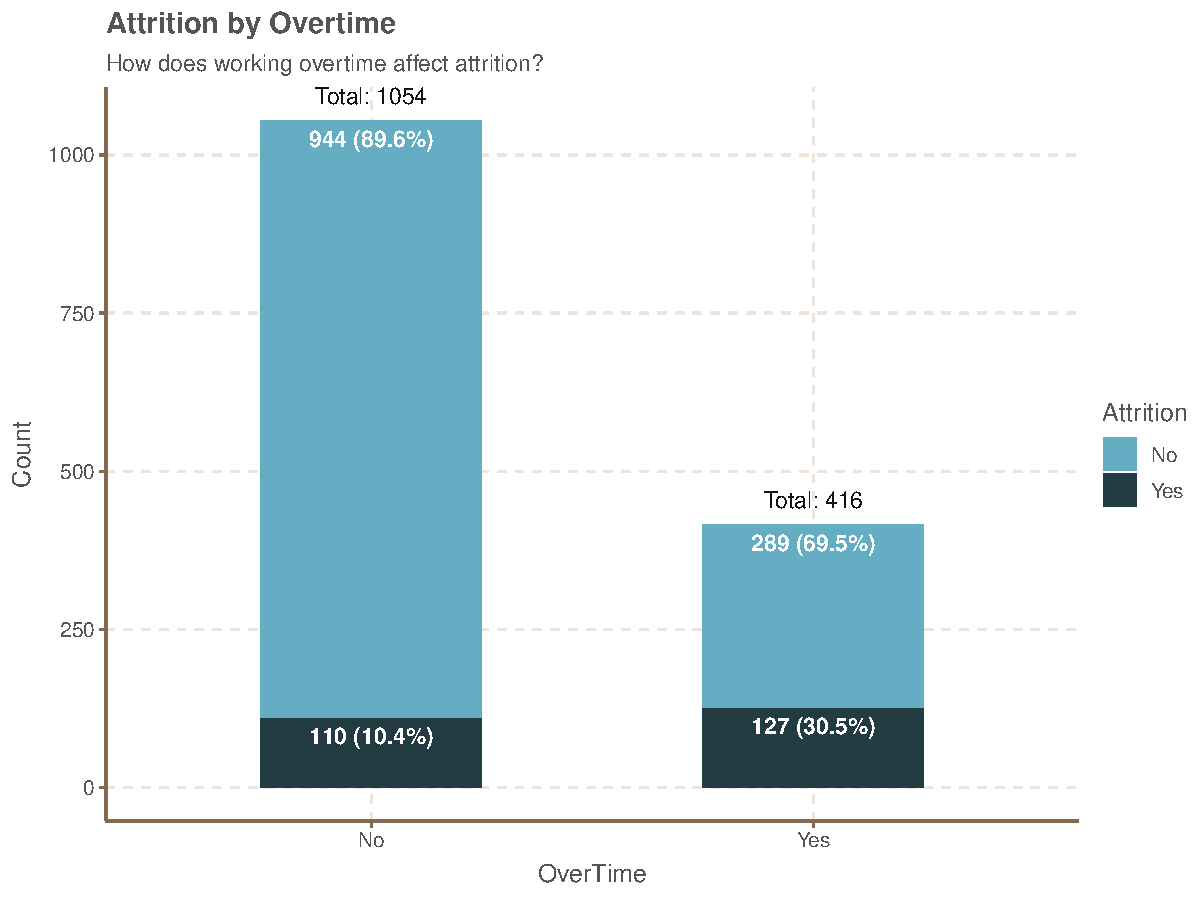
\includegraphics{figures/unnamed-chunk-16-1.pdf}

\textbf{Quick Takeaways:}

\begin{itemize}
\tightlist
\item
  Overall, 30.5\% of workers who worked overtime left the company in
  comparison to the 10.4\% of employees who never worked overtime.
\end{itemize}

\textbf{Overtime Distribution Within Company}

\begin{Shaded}
\begin{Highlighting}[]
\NormalTok{f_data }\OperatorTok
\StringTok{  }\KeywordTok{group_by}\NormalTok{(OverTime) }\OperatorTok
\StringTok{  }\KeywordTok{summarise}\NormalTok{(}\DataTypeTok{Count =} \KeywordTok{n}\NormalTok{()) }\OperatorTok
\StringTok{  }\KeywordTok{arrange}\NormalTok{(}\KeywordTok{desc}\NormalTok{(OverTime)) }\OperatorTok
\StringTok{  }\KeywordTok{mutate}\NormalTok{(}\DataTypeTok{ypos =} \KeywordTok{cumsum}\NormalTok{(Count)}\OperatorTok{-}\NormalTok{.}\DecValTok{5}\OperatorTok{*}\NormalTok{(Count)) }\OperatorTok
\StringTok{  }\KeywordTok{mutate}\NormalTok{(}\DataTypeTok{pct =} \KeywordTok{round}\NormalTok{(}\KeywordTok{prop.table}\NormalTok{(Count)}\OperatorTok{*}\DecValTok{100}\NormalTok{,}\DecValTok{1}\NormalTok{),}
    \DataTypeTok{label =} \KeywordTok{paste}\NormalTok{(Count, }\StringTok{" ("}\NormalTok{,pct, }\StringTok{"%"}\NormalTok{, }\StringTok{")"}\NormalTok{, }\DataTypeTok{sep =} \StringTok{""}\NormalTok{)) }\OperatorTok
\StringTok{  }\KeywordTok{ggplot}\NormalTok{(}\KeywordTok{aes}\NormalTok{(}\DataTypeTok{x =} \StringTok{""}\NormalTok{, }\DataTypeTok{y =}\NormalTok{ Count, }\DataTypeTok{fill =}\NormalTok{ OverTime), }\DataTypeTok{color =} \StringTok{"white"}\NormalTok{) }\OperatorTok{+}
\StringTok{  }\KeywordTok{geom_bar}\NormalTok{(}\DataTypeTok{stat =} \StringTok{"identity"}\NormalTok{, }\DataTypeTok{width =} \DecValTok{1}\NormalTok{) }\OperatorTok{+}
\StringTok{  }\KeywordTok{coord_polar}\NormalTok{(}\StringTok{"y"}\NormalTok{, }\DataTypeTok{start =}\DecValTok{0}\NormalTok{) }\OperatorTok{+}
\StringTok{  }\KeywordTok{geom_text}\NormalTok{(}\KeywordTok{aes}\NormalTok{(}\DataTypeTok{y =}\NormalTok{ ypos, }\DataTypeTok{label =}\NormalTok{ label), }\DataTypeTok{color =} \StringTok{"white"}\NormalTok{,}
    \DataTypeTok{fontface =} \StringTok{"bold"}\NormalTok{, }\DataTypeTok{size =} \DecValTok{4}\NormalTok{) }\OperatorTok{+}
\StringTok{  }\KeywordTok{labs}\NormalTok{(}\DataTypeTok{title =} \StringTok{"Percentage of Overtime Workers"}\NormalTok{, }\DataTypeTok{x =} \StringTok{""}\NormalTok{, }\DataTypeTok{y =} \StringTok{""}\NormalTok{) }\OperatorTok{+}\StringTok{ }
\StringTok{  }\KeywordTok{theme}\NormalTok{(}\DataTypeTok{axis.line =} \KeywordTok{element_blank}\NormalTok{(), }
    \DataTypeTok{axis.text.x =} \KeywordTok{element_blank}\NormalTok{(),}
    \DataTypeTok{axis.ticks =} \KeywordTok{element_blank}\NormalTok{(),}
    \DataTypeTok{axis.text.y =} \KeywordTok{element_blank}\NormalTok{(),}
    \DataTypeTok{panel.grid =} \KeywordTok{element_blank}\NormalTok{())}
\end{Highlighting}
\end{Shaded}

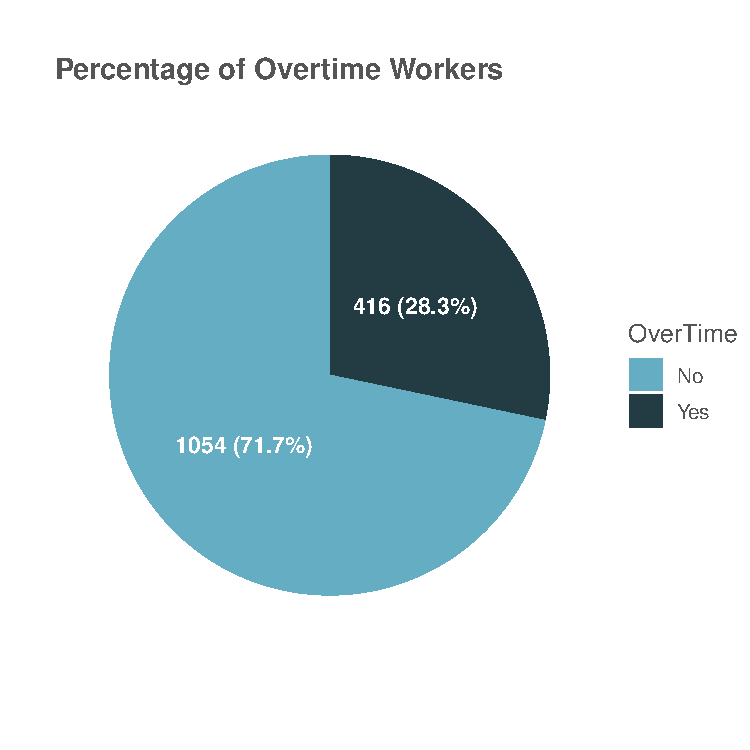
\includegraphics{figures/unnamed-chunk-17-1.pdf}

\textbf{Quick Takeaways:}

\begin{itemize}
\tightlist
\item
  28.3\% of the workforce worked overtime
\end{itemize}

\textbf{Overtime by Job Roles}

\begin{Shaded}
\begin{Highlighting}[]
\NormalTok{f_data }\OperatorTok
\StringTok{  }\KeywordTok{group_by}\NormalTok{(OverTime, JobRole) }\OperatorTok
\StringTok{  }\KeywordTok{summarise}\NormalTok{(}\DataTypeTok{Count =} \KeywordTok{n}\NormalTok{()) }\OperatorTok
\StringTok{  }\KeywordTok{group_by}\NormalTok{(JobRole) }\OperatorTok
\StringTok{  }\KeywordTok{arrange}\NormalTok{(Count) }\OperatorTok
\StringTok{  }\KeywordTok{mutate}\NormalTok{(}\DataTypeTok{CountPer =} \KeywordTok{prop.table}\NormalTok{(Count), }
    \DataTypeTok{label =} \KeywordTok{paste}\NormalTok{(}\StringTok{" ("}\NormalTok{, }\KeywordTok{round}\NormalTok{(CountPer}\OperatorTok{*}\DecValTok{100}\NormalTok{,}\DecValTok{0}\NormalTok{), }\StringTok{"%)"}\NormalTok{, }\DataTypeTok{sep =} \StringTok{""}\NormalTok{),}
    \DataTypeTok{total =} \KeywordTok{paste}\NormalTok{(}\StringTok{"Total:"}\NormalTok{, }\KeywordTok{sum}\NormalTok{(Count)),}
    \DataTypeTok{top =} \KeywordTok{sum}\NormalTok{(Count),}
    \DataTypeTok{JobRole =} \KeywordTok{gsub}\NormalTok{(}\StringTok{" "}\NormalTok{, }\StringTok{"}\CharTok{\textbackslash{}n}\StringTok{"}\NormalTok{, JobRole)) }\OperatorTok
\StringTok{  }\KeywordTok{ggplot}\NormalTok{(}\KeywordTok{aes}\NormalTok{(}\DataTypeTok{x =} \KeywordTok{as.factor}\NormalTok{(JobRole), }\DataTypeTok{y =}\NormalTok{ Count, }\DataTypeTok{fill =} \KeywordTok{as.factor}\NormalTok{(OverTime))) }\OperatorTok{+}
\StringTok{  }\KeywordTok{geom_bar}\NormalTok{(}\DataTypeTok{stat =} \StringTok{"identity"}\NormalTok{, }\DataTypeTok{position =} \StringTok{"dodge"}\NormalTok{, }\DataTypeTok{width =} \FloatTok{.5}\NormalTok{) }\OperatorTok{+}
\StringTok{  }\KeywordTok{geom_text}\NormalTok{(}\KeywordTok{aes}\NormalTok{(}\DataTypeTok{x =}\NormalTok{ JobRole, }\DataTypeTok{y =}\NormalTok{ Count, }
    \DataTypeTok{label =} \KeywordTok{ifelse}\NormalTok{(OverTime }\OperatorTok{==}\StringTok{ "Yes"}\NormalTok{, label, }\StringTok{""}\NormalTok{)),}
    \DataTypeTok{vjust =} \FloatTok{-.7}\NormalTok{, }\DataTypeTok{hjust =} \FloatTok{.05}\NormalTok{, }\DataTypeTok{color =} \StringTok{"black"}\NormalTok{, }\DataTypeTok{size =} \FloatTok{3.1}\NormalTok{) }\OperatorTok{+}
\StringTok{  }\KeywordTok{geom_text}\NormalTok{(}\KeywordTok{aes}\NormalTok{(}\DataTypeTok{x =}\NormalTok{ JobRole, }\DataTypeTok{y =}\NormalTok{ Count, }
    \DataTypeTok{label =} \KeywordTok{ifelse}\NormalTok{(OverTime }\OperatorTok{==}\StringTok{ "No"}\NormalTok{, label, }\StringTok{""}\NormalTok{)),}
    \DataTypeTok{vjust =} \DecValTok{-1}\NormalTok{, }\DataTypeTok{hjust=}\NormalTok{.}\DecValTok{70}\NormalTok{, }\DataTypeTok{color =} \StringTok{"black"}\NormalTok{, }\DataTypeTok{size =} \FloatTok{3.1}\NormalTok{) }\OperatorTok{+}
\StringTok{  }\KeywordTok{labs}\NormalTok{(}\DataTypeTok{title =} \StringTok{"Overtime by Job Roles"}\NormalTok{, }
    \DataTypeTok{subtitle =} \StringTok{"Are there particular roles that work overtime more often?"}\NormalTok{,}
    \DataTypeTok{x =} \StringTok{"Job Role"}\NormalTok{, }\DataTypeTok{fill =} \StringTok{"OverTime"}\NormalTok{) }\OperatorTok{+}
\StringTok{  }\KeywordTok{theme}\NormalTok{(}\DataTypeTok{axis.text.x =} \KeywordTok{element_text}\NormalTok{(}\DataTypeTok{size =} \DecValTok{9}\NormalTok{))}
\end{Highlighting}
\end{Shaded}

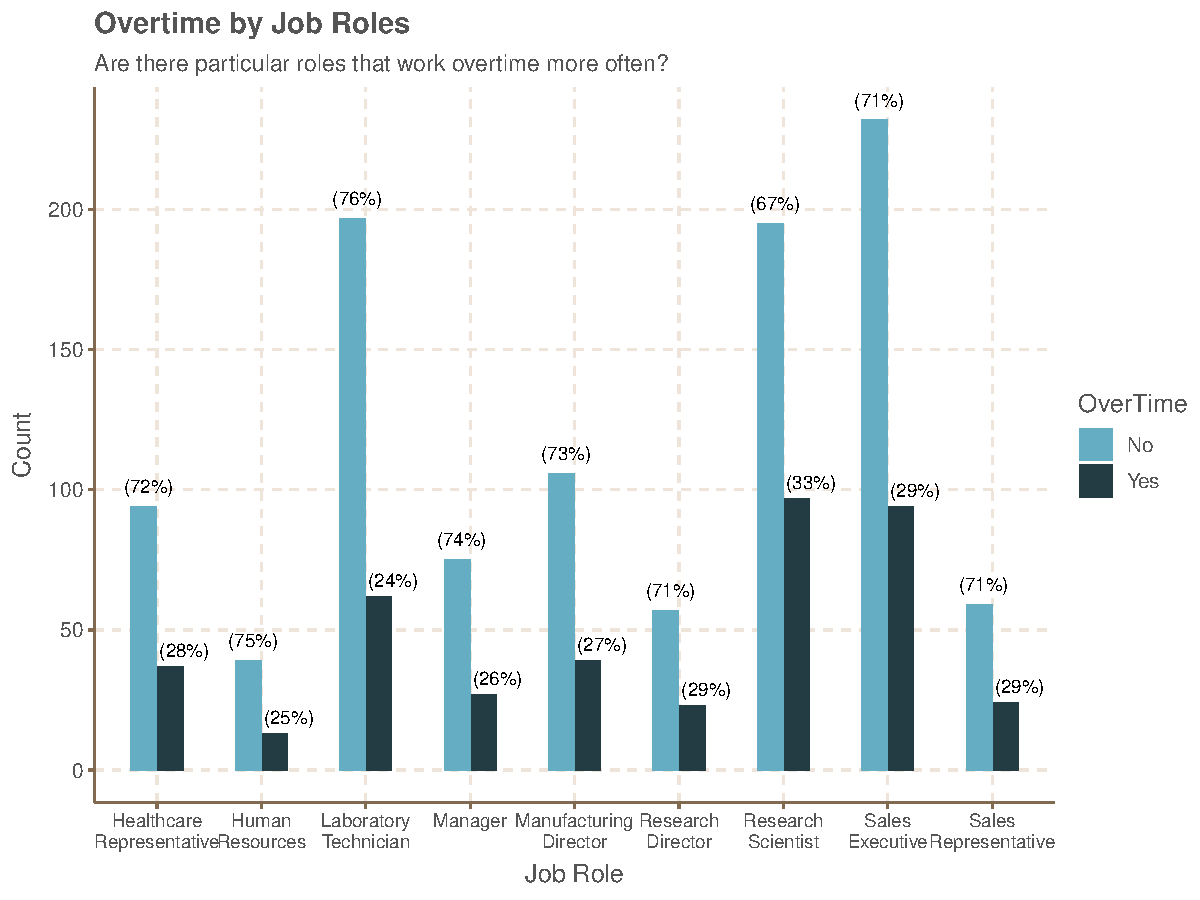
\includegraphics{figures/unnamed-chunk-18-1.pdf}

\textbf{Quick Takeaways:}

\begin{itemize}
\tightlist
\item
  Overall, all job roles had 25\%-33\% of their workforce work overtime
  with the highest being research scientists.
\end{itemize}

\textbf{Overtime by Job Levels}

\begin{Shaded}
\begin{Highlighting}[]
\NormalTok{f_data }\OperatorTok
\StringTok{  }\KeywordTok{group_by}\NormalTok{(OverTime, JobLevel) }\OperatorTok
\StringTok{  }\KeywordTok{summarise}\NormalTok{(}\DataTypeTok{Count =} \KeywordTok{n}\NormalTok{()) }\OperatorTok
\StringTok{  }\KeywordTok{group_by}\NormalTok{(JobLevel) }\OperatorTok
\StringTok{  }\KeywordTok{arrange}\NormalTok{(Count) }\OperatorTok
\StringTok{  }\KeywordTok{mutate}\NormalTok{(}\DataTypeTok{CountPer =} \KeywordTok{prop.table}\NormalTok{(Count), }
    \DataTypeTok{label =} \KeywordTok{paste}\NormalTok{(}\StringTok{" ("}\NormalTok{, }\KeywordTok{round}\NormalTok{(CountPer}\OperatorTok{*}\DecValTok{100}\NormalTok{,}\DecValTok{0}\NormalTok{), }\StringTok{"%)"}\NormalTok{, }\DataTypeTok{sep =} \StringTok{""}\NormalTok{),}
    \DataTypeTok{total =} \KeywordTok{paste}\NormalTok{(}\StringTok{"Total:"}\NormalTok{, }\KeywordTok{sum}\NormalTok{(Count)),}
    \DataTypeTok{top =} \KeywordTok{sum}\NormalTok{(Count)) }\OperatorTok
\StringTok{  }\KeywordTok{ggplot}\NormalTok{(}\KeywordTok{aes}\NormalTok{(}\DataTypeTok{x =} \KeywordTok{as.factor}\NormalTok{(JobLevel), }\DataTypeTok{y =}\NormalTok{ Count, }\DataTypeTok{fill =} \KeywordTok{as.factor}\NormalTok{(OverTime))) }\OperatorTok{+}
\StringTok{  }\KeywordTok{geom_bar}\NormalTok{(}\DataTypeTok{stat =} \StringTok{"identity"}\NormalTok{, }\DataTypeTok{position =} \StringTok{"dodge"}\NormalTok{, }\DataTypeTok{width =} \FloatTok{.5}\NormalTok{) }\OperatorTok{+}
\StringTok{  }\KeywordTok{geom_text}\NormalTok{(}\KeywordTok{aes}\NormalTok{(}\DataTypeTok{x =}\NormalTok{ JobLevel, }\DataTypeTok{y =}\NormalTok{ Count, }
    \DataTypeTok{label =} \KeywordTok{ifelse}\NormalTok{(OverTime }\OperatorTok{==}\StringTok{ "Yes"}\NormalTok{, label, }\StringTok{""}\NormalTok{)),}
    \DataTypeTok{vjust =} \FloatTok{-.7}\NormalTok{, }\DataTypeTok{hjust =} \FloatTok{.05}\NormalTok{, }\DataTypeTok{color =} \StringTok{"black"}\NormalTok{, }\DataTypeTok{size =} \FloatTok{3.1}\NormalTok{) }\OperatorTok{+}
\StringTok{  }\KeywordTok{geom_text}\NormalTok{(}\KeywordTok{aes}\NormalTok{(}\DataTypeTok{x =}\NormalTok{ JobLevel, }\DataTypeTok{y =}\NormalTok{ Count, }
    \DataTypeTok{label =} \KeywordTok{ifelse}\NormalTok{(OverTime }\OperatorTok{==}\StringTok{ "No"}\NormalTok{, label, }\StringTok{""}\NormalTok{)),}
    \DataTypeTok{vjust =} \DecValTok{-1}\NormalTok{, }\DataTypeTok{hjust=}\NormalTok{.}\DecValTok{9}\NormalTok{, }\DataTypeTok{color =} \StringTok{"black"}\NormalTok{, }\DataTypeTok{size =} \FloatTok{3.1}\NormalTok{) }\OperatorTok{+}
\StringTok{  }\KeywordTok{labs}\NormalTok{(}\DataTypeTok{title =} \StringTok{"Overtime by Job Levels"}\NormalTok{, }
    \DataTypeTok{subtitle =} \StringTok{"Are there particular levels that work overtime more often?"}\NormalTok{,}
    \DataTypeTok{x =} \StringTok{"Job Level"}\NormalTok{, }\DataTypeTok{fill =} \StringTok{"OverTime"}\NormalTok{) }\OperatorTok{+}
\StringTok{  }\KeywordTok{theme}\NormalTok{(}\DataTypeTok{axis.text.x =} \KeywordTok{element_text}\NormalTok{(}\DataTypeTok{size =} \DecValTok{9}\NormalTok{)) }\OperatorTok{+}
\StringTok{  }\KeywordTok{scale_y_continuous}\NormalTok{(}\DataTypeTok{limits =} \KeywordTok{c}\NormalTok{(}\DecValTok{0}\NormalTok{,}\DecValTok{500}\NormalTok{))}
\end{Highlighting}
\end{Shaded}

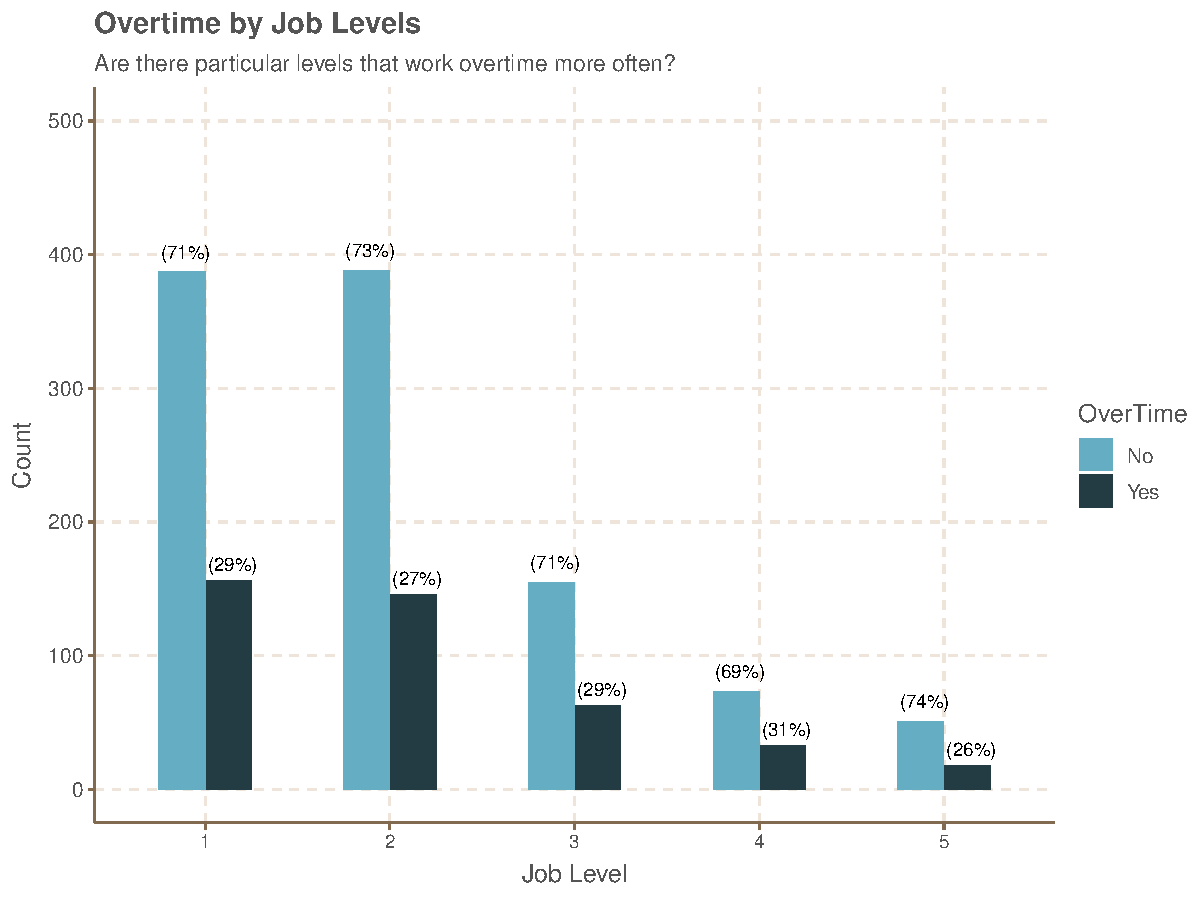
\includegraphics{figures/unnamed-chunk-19-1.pdf}

\textbf{Quick Takeaways:}

\begin{itemize}
\tightlist
\item
  Overall, all job levels had 25\%-31\% of their workforce work overtime
  with the highest being level 4.
\end{itemize}

\textbf{Average Job Satisfaction by Role \& Overtime}

\begin{Shaded}
\begin{Highlighting}[]
\NormalTok{f_data }\OperatorTok
\StringTok{  }\KeywordTok{group_by}\NormalTok{(OverTime, JobRole) }\OperatorTok
\StringTok{  }\KeywordTok{summarise}\NormalTok{(}\DataTypeTok{avg =} \KeywordTok{mean}\NormalTok{(JobSatisfaction))}\OperatorTok
\StringTok{  }\KeywordTok{ggplot}\NormalTok{(}\KeywordTok{aes}\NormalTok{(}\DataTypeTok{x =}\NormalTok{ OverTime, }\DataTypeTok{y =}\NormalTok{ avg, }\DataTypeTok{fill =}\NormalTok{ OverTime))}\OperatorTok{+}
\StringTok{  }\KeywordTok{geom_bar}\NormalTok{(}\DataTypeTok{stat =} \StringTok{"identity"}\NormalTok{) }\OperatorTok{+}
\StringTok{  }\KeywordTok{facet_wrap}\NormalTok{(}\KeywordTok{vars}\NormalTok{(JobRole)) }\OperatorTok{+}
\StringTok{  }\KeywordTok{labs}\NormalTok{(}\DataTypeTok{y =} \StringTok{"Average Job Satisfaction"}\NormalTok{, }
    \DataTypeTok{title =} \StringTok{"Average Job Satisfaction by Role & Overtime"}\NormalTok{,}
    \DataTypeTok{subtitle =} \StringTok{"Does working overtime affect job satisfaction?"}\NormalTok{)}
\end{Highlighting}
\end{Shaded}

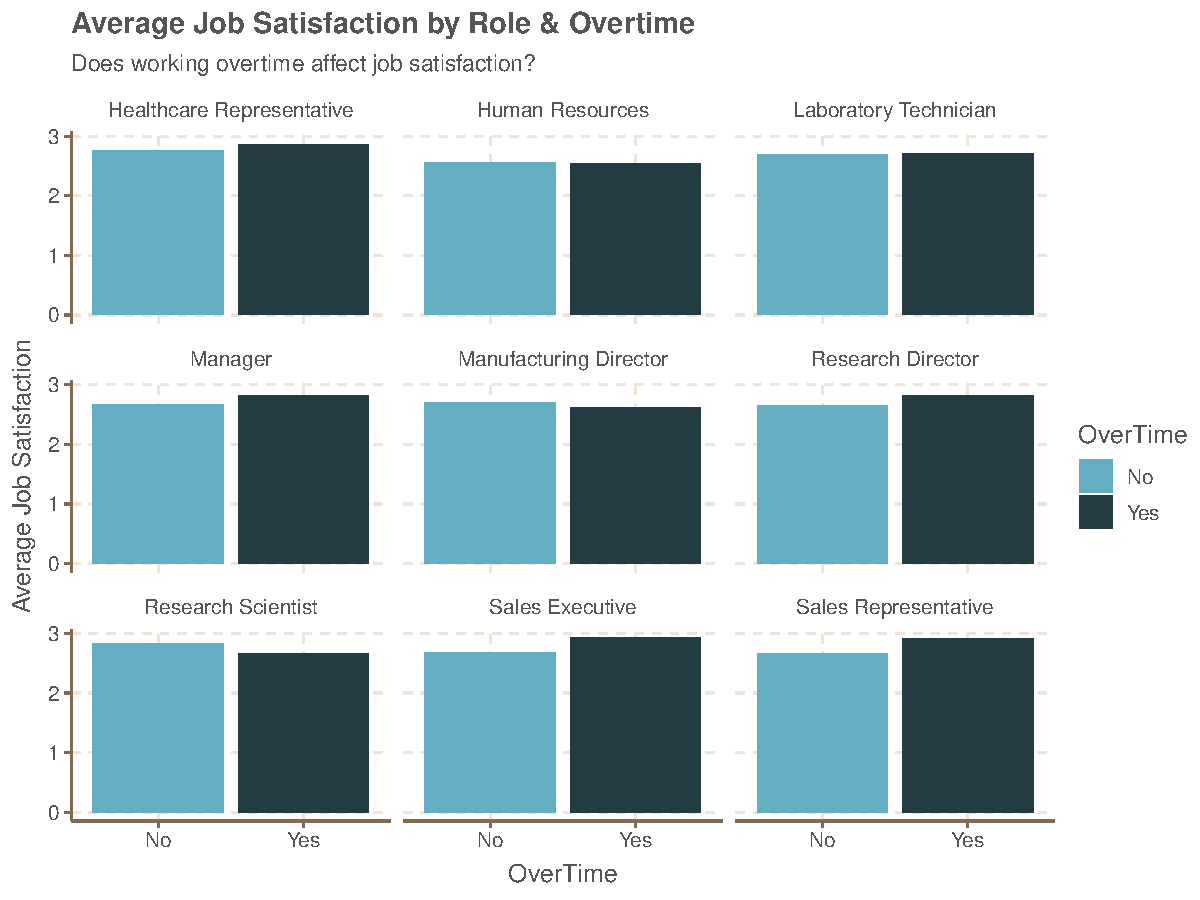
\includegraphics{figures/unnamed-chunk-20-1.pdf}

\textbf{Quick Takeaways:}

\begin{itemize}
\tightlist
\item
  Overall, job satisfaction does not seem to be impacted much by
  overtime.
\end{itemize}

\textbf{Average Environment Satisfaction by Role \& Overtime}

\begin{Shaded}
\begin{Highlighting}[]
\NormalTok{f_data }\OperatorTok
\StringTok{  }\KeywordTok{group_by}\NormalTok{(OverTime, JobRole) }\OperatorTok
\StringTok{  }\KeywordTok{summarise}\NormalTok{(}\DataTypeTok{avg =} \KeywordTok{mean}\NormalTok{(EnvironmentSatisfaction))}\OperatorTok
\StringTok{  }\KeywordTok{ggplot}\NormalTok{(}\KeywordTok{aes}\NormalTok{(}\DataTypeTok{x =}\NormalTok{ OverTime, }\DataTypeTok{y =}\NormalTok{ avg, }\DataTypeTok{fill =}\NormalTok{ OverTime))}\OperatorTok{+}
\StringTok{  }\KeywordTok{geom_bar}\NormalTok{(}\DataTypeTok{stat =} \StringTok{"identity"}\NormalTok{) }\OperatorTok{+}
\StringTok{  }\KeywordTok{facet_wrap}\NormalTok{(}\KeywordTok{vars}\NormalTok{(JobRole)) }\OperatorTok{+}
\StringTok{  }\KeywordTok{labs}\NormalTok{(}\DataTypeTok{y =} \StringTok{"Average Environment Satisfaction"}\NormalTok{, }
    \DataTypeTok{title =} \StringTok{"Average Environment Satisfaction by Role & Overtime"}\NormalTok{,}
    \DataTypeTok{subtitle =} \StringTok{"Does working overtime affect environment satisfaction?"}\NormalTok{)}
\end{Highlighting}
\end{Shaded}

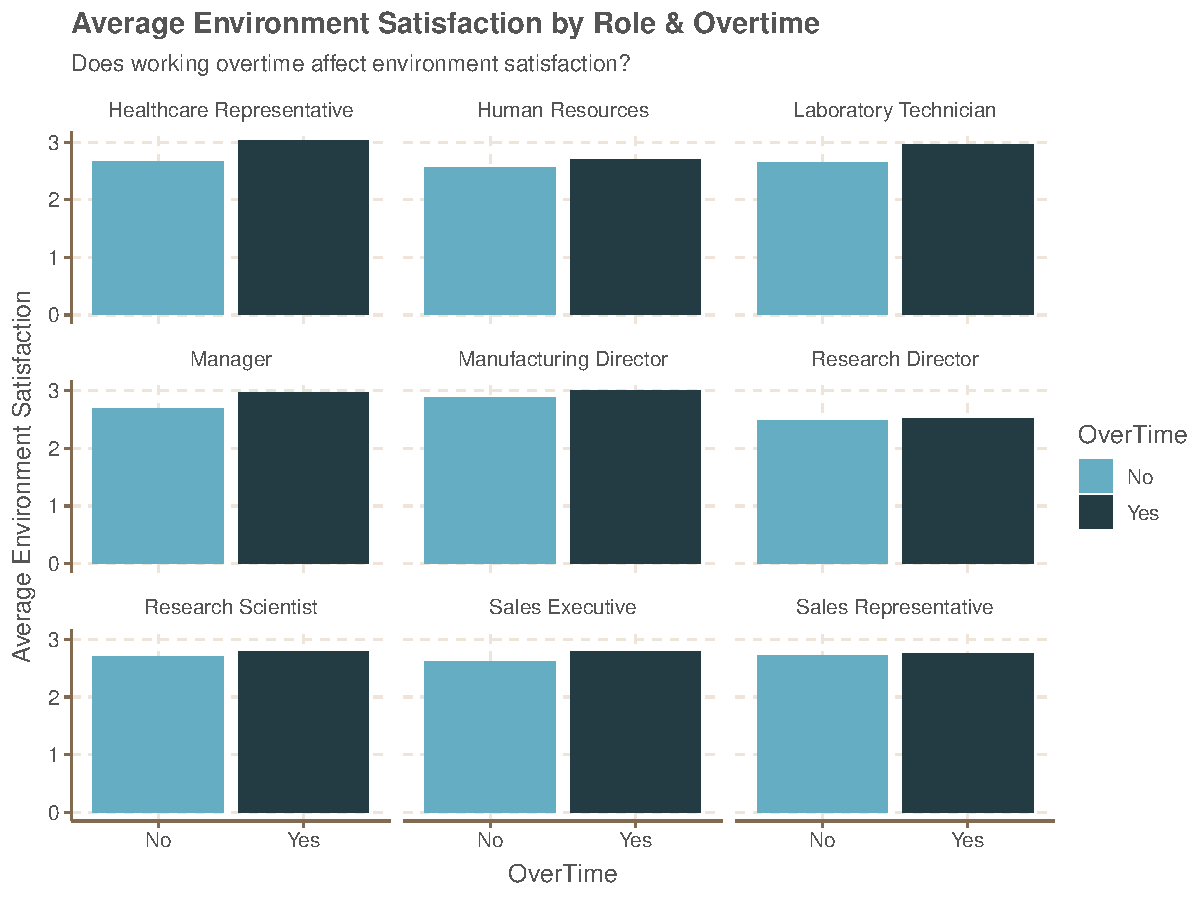
\includegraphics{figures/unnamed-chunk-21-1.pdf}

\textbf{Quick Takeaways:}

\begin{itemize}
\item
  \begin{itemize}
  \tightlist
  \item
    Overall, job environment satisfaction does not seem to be impacted
    much by overtime.
  \end{itemize}
\end{itemize}

\hypertarget{conlusions-next-steps}{%
\section{Conlusions: \& Next Steps}\label{conlusions-next-steps}}

\hypertarget{conclusions}{%
\subsection{Conclusions}\label{conclusions}}

After a preliminary exploratory data analysis, the following conclusions
seemed to be supported:

\begin{enumerate}
\def\labelenumi{\arabic{enumi}.}
\item
  The company's is losing a \textbf{large amount of young talent} as
  55\% of all attrition came from employees between 18-32. Also, 36\% of
  employees within the 18-25 age bracket as well as 22\% of employees
  within the 26-32 bracket left indicating the company's struggles
  maintaining younger talent
\item
  Sales representatives had the highest within attrition at 40\% with
  laboratory technician and human resources following at 24\% and 23\%.
  After investigation, \textbf{low income as well as low job
  satisfaction ratings may be strong contributors to the high attrition
  rate within sales representatives, laboratory technicians and human
  resources.}
\item
  \textbf{While environment satisfaction does seem to be a factor
  contributing to attrition across job roles, it was most evident for
  healthcare representatives and managers.} There was a large gap in
  environmental satisfaction between those healthcare representatives
  and managers who stayed and those who left. Further investigation on
  what environmental issues are negatively affecting those roles will be
  critical.
\item
  \textbf{While job satisfaction does seem to be a factor contributing
  to attrition across job roles, it was most evident for sales reps,
  laboratory technicians, and human resources.} There was a large gap in
  job satisfaction between those sales reps, laboratory technicians, and
  human resources who stayed and those who left. Further investigation
  on what issues are negatively affecting those roles will be critical.
\item
  Analysis shows that for the employees at IBM, \textbf{income did not
  have a strong influence on job satisfaction.} This suggests that low
  job satisfaction and income are two different factors.
\item
  Although I hypothesized that \textbf{job and environment satisfaction
  would be lower for those who worked overtime, that did not seem to be
  the case.} Further analysis on why job and environment satisfaction
  are low for certain job roles should be evaluated.
\item
  Altough overtime did not seem to affect job and environment
  satisfaction, a larger percent of those who worked overtime left the
  organization compared to those who didn't.
\end{enumerate}

\hypertarget{next-steps}{%
\subsection{Next Steps:}\label{next-steps}}

The purpose of the project was to conduct a preliminary analysis to
understand the data to guide future investigations. In addition, I
worked to create data visualizations to communicate the data to viewers.
All of the conclusions should be validated through a series of
point-biserial + pearson correlations, inferential statistics (t-tests),
and eventually linear + logistic regression models.\\
In addition, gathering qualitative data will be important as well. Exit
interview information as well as focus groups within job roles, levels,
and departments will help investigate questions we still have. For
example, qualitative data from exit interviews and focus groups may help
in:

\begin{enumerate}
\def\labelenumi{\arabic{enumi}.}
\tightlist
\item
  Understanding drivers of low job satisfaction especially within sales
  reps, laboratory technicians and human resources.
\item
  Understanding drivers of low environment satisfaction especially
  within healthcare representatives and managers.
\item
  Identifying potential culture issues or policies in place pushing
  younger talent away.
\item
  Confirming income as one of the most common drivers of attrition
\item
  Identifying reasons for why employees work overtime.
\end{enumerate}

\end{document}
